\documentclass[a4paper,12pt, twoside]{book}
\usepackage[T1]{fontenc} % package pour gérer les fontes
\usepackage{inputenc} % permet d'utiliser des caractères accentués dans le fichier source (.tex)
\usepackage{fontspec} % nécessaire pour utiliser des polices spécifiques avec XeLaTeX ou LuaLaTeX
\usepackage{lmodern} % charge la police Latin Modern, une version améliorée de Computer Modern
\usepackage[english,french]{babel} % gère la langue du document et ajuste les règles typographiques
\usepackage{appendix} % ajouter annexes
\usepackage{pdfpages} % inclure PDF
\usepackage{csquotes} % gère les citations
\usepackage{xspace} % gère les espaces après les commandes personnalisées
\usepackage{graphicx} % permet l'insertion d'images dans le document
\usepackage{setspace} % permet de gérer les paramètres de l'interligne
\usepackage{colortbl} % met de la couleur dans les lignes
\usepackage{caption} % met de sous titres dans les images, schémas etc.
    \captionsetup{font=small,labelfont=bf}

% Pour afficher le titre courant d'un chapitre non numéroté (intro, conclusion, etc.)
\usepackage{fancyhdr}
\pagestyle{fancy}
\fancyfoot{}
\fancyhead[RO,LE]{\thepage}
\fancyhead[LO]{\slshape \leftmark}
\fancyhead[RE]{\slshape \rightmark}
\renewcommand{\headrulewidth}{0pt}

\newcommand\mychapter[1]{%
  \chapter*{#1}%
  \markboth{\MakeUppercase{#1}}{\MakeUppercase{#1}} % markboth redéfinit à la fois les en-têtes gauche et droit
}

\usepackage[style=enc, sorting=nyt, maxbibnames=10]{biblatex} % charger le style de l'ENC
\addbibresource{03_bibliographie/shs_biblio.bib} % chemin pour l'inclusion de la bibliographie au fichier main.tex 
\addbibresource{03_bibliographie/techno.bib} % chemin pour l'inclusion de la bibliographie au fichier main.tex 


\usepackage{tocbibind} % pour l'inclusion de la liste des figures à la table des matière
\usepackage{hyphenat} % césuration de mots automatique
\hyphenation{mathéma-tiques récu-pérer}

\usepackage{lipsum} % pour l'inclusion de texte aléatoire, c'était important pendant les phases de test

\usepackage[pdfusetitle, pdfsubject={Mémoire TNAH — Vers une persistance numérique des collections : Développement d'outils IIIF au sein du DaSCH}, pdfkeywords={IIIF, persistance de données, green coding, gestion de données, Python, HTML, CSS, JavaScript, front end}]{hyperref}

\usepackage{listings} % permet de formater et afficher du code source.
\usepackage{xcolor} % permet de gérer et personnaliser les couleurs dans un document LaTeX.

% Configuration des couleurs et du style pour le code Python

%%%% Code crée à l'aide de ChatGPT : %%%%%
% Définir des couleurs personnalisées avec des codes hexadécimaux
\definecolor{mybackground}{HTML}{a9a9a9} % Couleur de fond
\definecolor{mykeyword}{HTML}{b44de0}    % Couleur des mots-clés

% Style pour Python
\lstdefinestyle{mystyle}{
    backgroundcolor=\color{mybackground},   % Couleur de fond
    commentstyle=\color{green},          % Style des commentaires
    keywordstyle=\color{mykeyword}\bfseries,  % Style des mots-clés
    numberstyle=\tiny\color{gray},       % Style des numéros de lignes
    stringstyle=\color{yellow},             % Style des chaînes de caractères
    basicstyle=\ttfamily\footnotesize,   % Style de base du texte
    breaklines=true,                     % Retour à la ligne automatique
    language=Python                      % Langage du code
}

\lstset{style=mystyle} % 

%%%%%

% commande pour l'italique en texte en anglais
\newcommand{\eng}{\emph} 

% applications et logiciels
\newcommand{\cvt}{{DaSCH Converter}\xspace}
\newcommand{\msh}{DaSCH Mesh\xspace}
\newcommand{\diiif}{DaSCH IIIF\xspace}
\newcommand{\bld}{Blender\xspace}
\newcommand{\gmp}{GIMP\xspace}
\newcommand{\mlb}{MeshLab\xspace}

% stage 
\newcommand{\dsc}{DaSCH\xspace}
\newcommand{\rg}{Rita Gautschy\xspace}
\newcommand{\enc}{École nationale des chartes\xspace}
\newcommand{\tnah}{\textsc{tnah}\xspace}
\newcommand{\DSC}{\eng{Swiss National Data and Service Center for the Humanities}\xspace}
\newcommand{\dhlab}{\eng{Digital Humanities Lab} (DHLab)\xspace}
\newcommand{\erid}{\eng{ERI Dispatch}\xspace}
\newcommand{\ERID}{l'\eng{ERI} (\eng{Education}, \eng{Research and Innovation}) \eng{Dispatch}\xspace}
\newcommand{\iiif}{\eng{International Image Interoperability Framework}\xspace}
\newcommand{\psdn}{persistance de données\xspace}
\newcommand{\sagw}{\eng{Swiss Academy of Humanities and Social Sciences} (SAGW)\xspace}
\newcommand{\SNSFn}{\eng{Swiss National Science Foundation} (SNSF)\xspace}
\newcommand{\unibas}{Universität Basel\xspace}

% Concepts
\newcommand{\gco}{\eng{green coding}\xspace}
\newcommand{\gwsh}{\eng{greenwashing}\xspace}
\newcommand{\opso}{\eng{open source}\xspace}
\newcommand{\opdt}{\eng{Open Data}\xspace}
\newcommand{\be}{\eng{back end}\xspace}
\newcommand{\fe}{\eng{front end}\xspace}
\newcommand{\g}[1]{\og#1~\fg}
\newcommand{\ux}{\eng{UX}\xspace}
\newcommand{\p}{[\ldots]\xspace}

% IIIF concepts
\newcommand{\iapit}{\eng{Image API 3.0}\xspace}
\newcommand{\iapiq}{\eng{Image API 4.0}\xspace}
\newcommand{\papit}{\eng{Presentation API 3.0}\xspace}
\newcommand{\papiq}{\eng{Presentation API 4.0}\xspace}

% langages de programmation
\newcommand{\css}{\textsc{css}\xspace}
\newcommand{\html}{\textsc{html}\xspace}
\newcommand{\JS}{\textsc{JavaScript}\xspace}
\newcommand{\py}{\textsc{Python}\xspace}

% commandes pour les bibliothèques liées à Python
\newcommand{\bs}{\textsc{Bootstrap}\xspace}
\newcommand{\fsk}{\textsc{flask}\xspace}
\newcommand{\FSK}{\textsc{Flask}\xspace}

\lstdefinestyle{mystyle}{
    backgroundcolor=\color{lightgray},   % Cor de fundo
    commentstyle=\color{green},          % Estilo de comentário
    keywordstyle=\color{blue}\bfseries,  % Estilo de palavras-chave
    numberstyle=\tiny\color{gray},       % Estilo dos números das linhas
    stringstyle=\color{red},             % Estilo das strings
    basicstyle=\ttfamily\footnotesize,   % Estilo básico do texto
    breaklines=true,                     % Quebra automática de linhas
    language=Python                      % Linguagem do código
}

% pour retirer le titre courant d'une page vide avant un chapitre
% modèle copié de https://github.com/Segolene-Albouy/Memoire-TNAH2019/blob/master/memoire.tex
\newcommand{\clearemptydoublepage}{\newpage{\pagestyle{empty}\cleardoublepage}}

% informations de la page de titre
\title{Vers une persistance numérique des collections : Développement d'outils IIIF au sein du DaSCH}
\author{Gilmar Ballestrim}
\date{Septembre 2024}

\begin{document}

    % inclusion des parties de la disseration au fichier main.tex
    \onehalfspacing 
	
    \frontmatter
	\begin{titlepage}
		\begin{center}
			
			\bigskip
			
			\begin{large}
				ÉCOLE NATIONALE DES CHARTES
			\end{large}
			\begin{center}\rule{5cm}{0.02cm}\end{center}
			
			\bigskip
			\bigskip
			\bigskip
			\begin{Large}
				\textbf{Gilmar Ballestrim}\\
			\end{Large}
            \begin{normalsize} \textit{Licencié en histoire à l'Universidade de São Paulo}\\
			\end{normalsize}

			\bigskip
			\bigskip
			\bigskip
			
			\begin{Huge}
				\textbf{Vers une persistance numérique des collections :}\\
			\end{Huge}
			\bigskip
			\bigskip
			\begin{LARGE}
				\textbf{Développement d'outils IIIF au sein du DaSCH}\\
			\end{LARGE}
			
			\bigskip
			\bigskip
			\bigskip
			\begin{large}
			\end{large}
			\vfill
			
			\begin{large}
				Mémoire 
				pour le diplôme de master \\
				\og {Technologies numériques appliquées à l'histoire} \fg \\
				\bigskip
				Septembre 2024
			\end{large}
			
		\end{center}
	\end{titlepage}

 
    \clearemptydoublepage
    
    \chapter*{Résumé}
\addcontentsline{toc}{chapter}{Résumé}
\medskip
        Dans le cadre de mon stage au sein du \dsc, j'ai développé trois applications visant à permettre à des versions allégées d'images 2D et objets 3D d'intégrer leurs métadonnées structurelles et descriptives au cadre international d'interopérabilité des images (\iiif~- IIIF). La question de recherche est la suivante : est-il réellement possible de garantir la \psdn archivistiques en utilisant IIIF ?\\
        
        Le principal défi aujourd'hui réside dans la gestion de données hétérogènes provenant d'objets intrinsèquement variés, ainsi que de différentes organisations ayant des objectifs distincts. L'enjeu est d'éviter l'effet \enquote{\eng{setting and forgetting}} en cherchant à rendre la description et l'exploitation des données pérennes entre diverses organisations. De plus, l'utilisation de ces données soulève des problèmes et des impacts environnementaux. Par conséquent, l'optimisation de la préservation numérique et de l'interopérabilité apparaît comme une priorité à développer, car elle permettrait une utilisation efficace des données dans un contexte patrimonial.\\

        \textbf{Mots-clés:} IIIF~; \psdn~; \gco~; gestion de données~; \py~; \html~; \css~; \JS~; \fe~.\\
	
    	\textbf{Informations bibliographiques~:} Gilmar Ballestrim, \textit{Vers une persistance numérique des collections}, mémoire de Master \g{Technologies numériques appliquées à l'histoire}, dir. Edward Gray, \enc, septembre 2024.

    \clearemptydoublepage
    
    \chapter*{Abstract}
\addcontentsline{toc}{chapter}{Abstract}
\medskip
    During my internship at the \dsc, I developed three applications aimed at enabling lighter versions of 2D images and 3D objects to integrate their structural and descriptive metadata into the International Image Interoperability Framework (\iiif~- IIIF). The research question is as follows: Is it truly possible to ensure archival data persistence using IIIF?\\
    
    The main challenge today lies in managing heterogeneous data from intrinsically varied objects and different organizations with distinct objectives. The goal is to avoid the \enquote{\eng{setting and forgetting}} effect by striving to make data description and utilization sustainable across various organizations. Additionally, the use of this data raises environmental issues and impacts. Therefore, optimizing digital preservation and interoperability emerges as a priority to be developed, as it would allow for the efficient use of data in a heritage context.\\

\textbf{Keywords:} IIIF~; data persistence~; \gco~; data management~; \py~; \html~; \css~; \JS~; \fe~.\\

\textbf{Bibliographic Information:} Gilmar Ballestrim, \textit{Towards Digital Persistence of Collections}, Master's thesis in \g{Digital Technologies Applied to History}, dir. Edward Gray, \enc, September 2024.

    \clearemptydoublepage
    
    % TALVEZ ESTILIZAR

\chapter{Dédicace}
    
     Tout comme le titre du livre de l'écrivain portugais Valter Hugo Mãe, je me sens aussi un fils de mille hommes, mais j'ajoute : aussi de mille femmes.\\
     
     Je souhaite dédier ces premiers lignes, à ceux et celles qui m'ont permis d'écrire toutes les lignes restantes de ce travail. À ceux et celles qui, par leur travail physique, dès l'enfance, m'ont permis d'avoir un travail intellectuel à un moment de ma vie.\\
     
     Ces lignes symbolisent non seulement la liberté, mais aussi de nouvelles pages dans ma vie.\\
     
     À mes deux grands-pères disparus, Chico et Jobel, qui m'ont donné des trésors invisibles qui demeurent au cœur de ma vie. Un jour, j'ai promis à l'un d'eux que je serai le premier de la famille à entrer à l'université et, aujourd'hui, je peux dire que j'ai osé aller plus loin. Merci.\\
    
    \begin{flushright}
    Avec amour, \\
    Gil.
    \end{flushright}
    \clearemptydoublepage
    
    \chapter{Remerciements}

C’est avec une profonde gratitude que je tiens à remercier toutes les personnes qui ont contribué à la réalisation de ce mémoire de master.

Je tiens tout d'abord à exprimer ma gratitude au corps professoral de l’\enc, en particulier à Emmanuelle Bermès, pour leur soutien académique et leur bienveillance.

Je souhaite exprimer ma sincère reconnaissance à mon directeur de mémoire, le Professeur Dr. Edward Gray, pour son encadrement éclairé, ses conseils précieux et ses corrections tout au long de ce parcours. Son expertise et son expérience ont été déterminantes pour mener à bien ce travail.

Je remercie chaleureusement Rita Gautschy, ma cheffe de stage, pour son aide inestimable, sa confiance et les échanges enrichissants que nous avons eus. Je suis également très reconnaissant envers Daniela Meier et Gaby de l’IAESTE pour leur assistance qui a rendu mon séjour à Bâle des plus agréables. Enfin, je tiens à remercier toute l’équipe du \dsc pour les bons moments passés pendant mon stage, et en particulier Julien Raemy pour ses conseils avisés et nos échanges fructueux.

Mes remerciements vont également à mes amis et collègues de l’\enc, en particulier à Anna, Marina et Sarah, pour leur soutien, les discussions et les échanges qui ont été très importants. Je remercie également Amos et Karim pour les discussions très agréables que nous avons eues tout au long de cette année.

Je voudrais exprimer ma gratitude à l’équipe de la Communication de l’\enc, notamment à David, pour leur soutien dans le cadre de mon premier emploi en tant que développeur.

Je remercie mes amis et collègues de l’Université de São Paulo, Denilton Donizetti, Gustavo Vicente, Jeferson Benevides, Johnny Esteves, Lucas Soares, Lucas Gandolfi, Thiago Marinho Del Corso, Thiago Kenji, Tomas Mistrorigo, Tomas Pinho et William Valério, pour les moments de partage et les discussions enrichissantes qui ont marqué cette période d’études.

Je souhaite remercier du fond du cœur Addison, Alice, Antônio, Carla, Caroline, Gabriel Bassan, Gabriel Perli, Isaure, João, José Victor, Miguel, Nordine, Pietro Piccioni, Plínio, Rafael et Vitor Sanches pour leur amitié et leur soutien inconditionnel dans les différents moments de ma vie en France.

Un grande merci à mes amis et amies, Camilo, Gabriel Cruz, Gabriel Perli, Greicy Lins, João Pedro et Renata Cavazzana. Votre présence à mes côtés, votre écoute attentive et vos encouragements sans faille ont été les piliers de cette aventure.

Je tiens à exprimer ma profonde gratitude à mes parents, Inês et Osmar, pour leur amour, leur confiance et leur soutien inconditionnel dans tous mes choix.

Un immense merci à Laurène pour ses encouragements, son aide précieuse et sa patience. Sa présence à mes côtés a été inestimable.

Je remercie toutes les institutions qui ont contribué à ce projet, notamment la Société d’Entraide de l’École des chartes, en particulier Isabelle Le Masne de Chermont, Camille Dégez-Selves et Solange Bidou. Je remercie également Florian Bourguignon et l'agence Erasmus. Leur soutien moral et financier a été inestimable et précieux pour moi.

Finalement, je remercie Edward Gray, Rita Gautschy, Gabriel Perli et Laurène pour leur relecture.
    \clearemptydoublepage
    
    \mychapter{Introduction}
\addcontentsline{toc}{chapter}{Introduction}

    Programmer, dans notre société contemporaine, ne se résume plus à écrire des lignes de code : c’est également une activité qui s’inscrit dans un contexte social, politique et environnemental complexe. L’essor du concept de \gco met en lumière la nécessité de prendre en compte les impacts environnementaux et sociaux de la production de logiciels. C'est pour cette raison que dans le cadre de mon stage au sein du \DSC, j'ai été amené à développer deux applications éco-responsables visant à intégrer des versions allégées d'images 2D et modèles 3D, ainsi que leurs métadonnées structurelles et descriptives, au sein du cadre international d'interopérabilité des images, connu sous le nom d'\iiif~(IIIF). Ce travail s'inscrit dans une problématique plus large, soulevée par la question de recherche suivante : est-il réellement possible de garantir la persistance des données archivistiques en utilisant IIIF ?\\

    Cette interrogation prend toute son importance dans le contexte actuel, où la gestion de données hétérogènes constitue un défi majeur. Ces données, issues d'objets intrinsèquement variés et de différentes organisations, posent des problèmes d'harmonisation et de pérennisation. Le défi réside notamment dans la nécessité d'éviter l'effet \enquote{\eng{setting and forgetting}}, c'est-à-dire l'abandon de données après leur archivage initial, en développant des solutions qui assurent une description et une exploitation durable des informations à travers diverses organisations. De plus, l'usage de ces données numériques soulève des questions environnementales, rendant l'optimisation de leur préservation et interopérabilité une priorité.\\

    En outre, programmer est aussi une activité qui s'inscrit dans un moment historique précis. Les codes conçus ont pour but la préservation patrimoniale : bien qu'ils aient une finalité spécifique, ils sont souvent crées dans les contextes collectifs et d'\opso et sont susceptibles de devenir une marchandise. Cette discussion sera approfondie, mais on peut dès à présent souligner que rares sont les questionnements concernant les effets de la codification et la manière dont elle masque les relations sociales qui impactent, directement ou indirectement, non seulement l’environnement, mais aussi la vie des individus. Autrement dit, la réflexion de cette étude n'est pas d'épuiser le sujet de la relation entre la programmation et l'environnement, puisque cela est un débat déjà connu, notre idée est plutôt de mettre en exergue le fait que ces deux dimensions sont forcément liées à un mode de reproduction historique de la vie. En effet, comme Karl Marx l’avait souligné, les idées ne surgissent pas dans le vide, mais sont enracinées dans la réalité matérielle \footnote{Pour Marx, les Jeunes-Hégéliens restaient enfermés dans une pure spéculation philosophique, sans chercher à relier leurs idées à la société concrète dans laquelle ils vivaient. C'est de là que vient la célèbre phrase de Marx \enquote{Ce que sont les individus dépend donc des conditions matérielles de leur production} \cite[p.~44-45]{marx1968}.}. Dans notre société, les moyens de production sont principalement capitalistes. Si le capitalisme n'est pas un système transhistorique, comme l'a également souligné Moishe Postone \footnote{A l'instar de Postone, la théorie du travail qui intéresse cette étude est celle historiquement spécifique à la société capitaliste, non une sorte de capitalisme qui s'étend à toutes les sociétés de forme transhistorique. C'est justement cette dernière notion qui représente la critique centrale du livre de l'auteur. En outre, cette théorie va de pair avec la notion qui implique que le capitalisme est l'une des caractéristiques de base de la modernité \cite[p.~9-21]{postone1996}.}, il imprègne une grande partie des relations sociales, dont la programmation est l'une des manifestations.\\
    
    Toutefois, ce travail tente de penser des possibilités pour restituer un autre mode de programmation dans cette configuration sociale. Or, l’histoire de la programmation évidemment n'est pas une simple histoire de la guerre ou du capitalisme. Les discussions sur l’utilisation des logiciels libres et \opso, à l'instar des \eng{Free Open Source Software} (FOSS), ont une histoire liée à la contre-culture aux États-Unis : ces aspirations suggéraient beaucoup plus l’idée d’une quête pour la liberté des individus que de répondre aux aspirations capitalistes \footnote{Voir \cite{shi2014mainstreaming}.}.\\

    De plus, ce mémoire est également le moment de remettre en question certains concepts tels que le document, l'objet et l'artefact : ces définitions, qui font l'objet de débats terminologiques depuis longtemps, sont de plus en plus placées dans un contexte d'études interdisciplinaires. Un exemple de ce que nous explorerons et défendrons dans ce travail est le champ interdisciplinaire de la culture matérielle, qui nous intéresse de près, car ces définitions englobent des dimensions historiques qui influent sur les manières dont nous conservons les choses avec lesquelles nous interagissons et, par conséquent, sur la façon dont nous transformons ces choses en données ou comment nous concevons les données, puisque les données présentent ces deux aspects non négligeables : celui de choses qui sont devenues numériques ou celui de choses qui naissent numériques.\\
    
    Ce mémoire est structuré en trois parties principales, chacune visant à explorer en profondeur les différentes dimensions du travail effectué et à situer les développements réalisés dans leur contexte théorique et pratique.\\
    
    La première partie, intitulée \textbf{Production au sein du \dsc}, se concentre sur la mise en place du cadre institutionnel et technologique dans lequel s'inscrit ce projet. Cette section commence par un examen détaillé du \dsc, une institution suisse dédiée à la préservation numérique du patrimoine culturel. Le premier chapitre retrace l'histoire et la fondation du \dsc, en mettant l'accent sur ses liens avec l'initiative de l'\opdt en Suisse et sur les modèles de financement qui soutiennent ses activités. Ensuite, le contexte technique du IIIF est introduit. Ce cadre d'interopérabilité, crucial pour la gestion et le partage des images patrimoniales, est présenté à travers ses différentes versions, depuis l'API 3.0 jusqu'aux développements envisagés pour l'API 4.0. Enfin, cette partie aborde les concepts fondamentaux liés à la persistance des données numériques, en clarifiant les distinctions entre documents, objets et données, tout en soulignant les défis posés par la numérisation du patrimoine. Une attention particulière est mise sur les enjeux spécifiques du stage, les objectifs des \eng{pipelines} développés, et les limitations rencontrées dans l'automatisation des processus à travers l'utilisation de technologies comme \py, \textsc{flask}, \textsc{bootstrap}, et \textsc{docker}.\\
    
    La deuxième partie, dont le titre est \textbf{De l'image au standard IIIF : conceptions des \eng{pipelines} de traitement}, se consacre à l'aspect technique du projet, détaillant la conception et la mise en œuvre des \eng{pipelines} de traitement d'images pour leur intégration dans le standard IIIF. Cette section se divise en plusieurs chapitres qui expliquent, étape par étape, le processus d'optimisation des images et des objets numériques pour répondre aux exigences du IIIF. Elle explore notamment le développement des outils \cvt et \msh, qui ont été conçus pour faciliter cette intégration. Une attention particulière est accordée à la structure de ces outils, à leur architecture logicielle, ainsi qu'à l'expérience utilisateur. Finalement, la discussion porte sur les défis techniques et des solutions apportées pour enrichir les métadonnées et alimenter les manifestes IIIF lors de la conception d'\diiif.\\
    
    La troisième partie, formulée en tant qu'\textbf{Évaluation des outils et méthodes : bilan et perspectives}, propose une analyse critique des résultats obtenus au cours du développement des applications et aussi une réflexion à propos des outils de gestion du temps. Elle commence par une évaluation de la performance des outils créés, en examinant leur efficacité, leur robustesse et leur capacité à répondre aux objectifs initiaux du projet. Est discutée ensuite la façon dont les outils de gestion ont été intégrés lors du stage. Cette partie se poursuit avec une réflexion sur les perspectives d'évolution des outils, en identifiant des fonctionnalités supplémentaires qui pourraient être développées pour améliorer encore davantage l'intégration des images et métadonnées dans le cadre IIIF. Enfin cette section se termine sur des pistes de recherches futures, en considérant l'impact potentiel des technologies explorées sur la préservation du patrimoine culturel numérique.\\
    
    Ce mémoire vise ainsi à fournir une analyse des enjeux techniques et institutionnels liés à la gestion des données patrimoniales numériques, tout en proposant des solutions éco-resposables pour améliorer leur interopérabilité et leur préservation à travers l'utilisation du standard IIIF, sans oublier la dimension historique sous-jacente à cette reproduction historique de vie.
    \clearemptydoublepage
    
    % REVISAR OS ESPACOS ENTRE O TEXTO E O PONTO FINAL!
% REVISAR OS NOMES EM INGLES, POR EXEMPLO : DESKTOP, SOFTWARE! ET COLOCAR ENG QUANDO FOR O CASO
\mainmatter
\part{Production au sein du \dsc}
\chapter{Contexte \dsc}
    \section{Qu'est-ce que \dsc ?}
    
    Le \DSC, connu sous l'acronyme \dsc, est une est une infrastructure nationale sans but lucratif pour les données de recherche en sciences humaines, axée sur les données qualitatives en Suisse, c'est-à-dire les données \eng{bitstream} telles que les images, l'audio, la vidéo et texte.
    
    La mission de \dsc est essentielle au développement d'une infrastructure de recherche numérique fiable et ouverte pour les sciences humaines en Suisse. En tant que dépositaire de données de recherche, \dsc s'engage à assurer un accès direct et durable aux données tout en permettant leur modification continue.\footnote{Voir \cite{daschmission}.} Cette mission est renforcée par l'accent mis sur l'interopérabilité et l'utilisation de normes reconnues, garantissant ainsi une intégration fluide avec les outils existants utilisés par les communautés scientifiques. De plus, l'engagement de \dsc dans la promotion des données ouvertes et dans la formation à la gestion des données de recherche témoigne de son rôle central dans l'écosystème de la recherche numérique en Suisse. Ce rôle est encore amplifié par la collaboration étroite avec les communautés de recherche, tant au niveau national qu'international, ce qui permet de maintenir une plateforme en constante évolution, adaptée aux besoins changeants des chercheurs.
    
    Les valeurs de \dsc constituent le fondement de sa mission et guident toutes ses actions. La fiabilité est au cœur de l'engagement de \dsc envers ses utilisateurs, assurant une communication transparente et le respect des délais. Cette fiabilité est complétée par une flexibilité qui permet à \dsc de répondre efficacement aux besoins spécifiques des chercheurs, en envisageant des alternatives et en proposant des scénarios adaptés. L'appréciation et la curiosité, quant à elles, favorisent un environnement de travail constructif et innovant, où les besoins des chercheurs sont constamment pris en compte et où l'exploration de nouvelles technologies est encouragée.

    Pour comprendre comment la mission et les valeurs de l'association s'alignent avec d'autres aspects, y compris sa fondation, nous allons procéder à une brève analyse de la gouvernance de \dsc.

    % logo du \dsc
    \begin{figure}[h!]
        \centering
        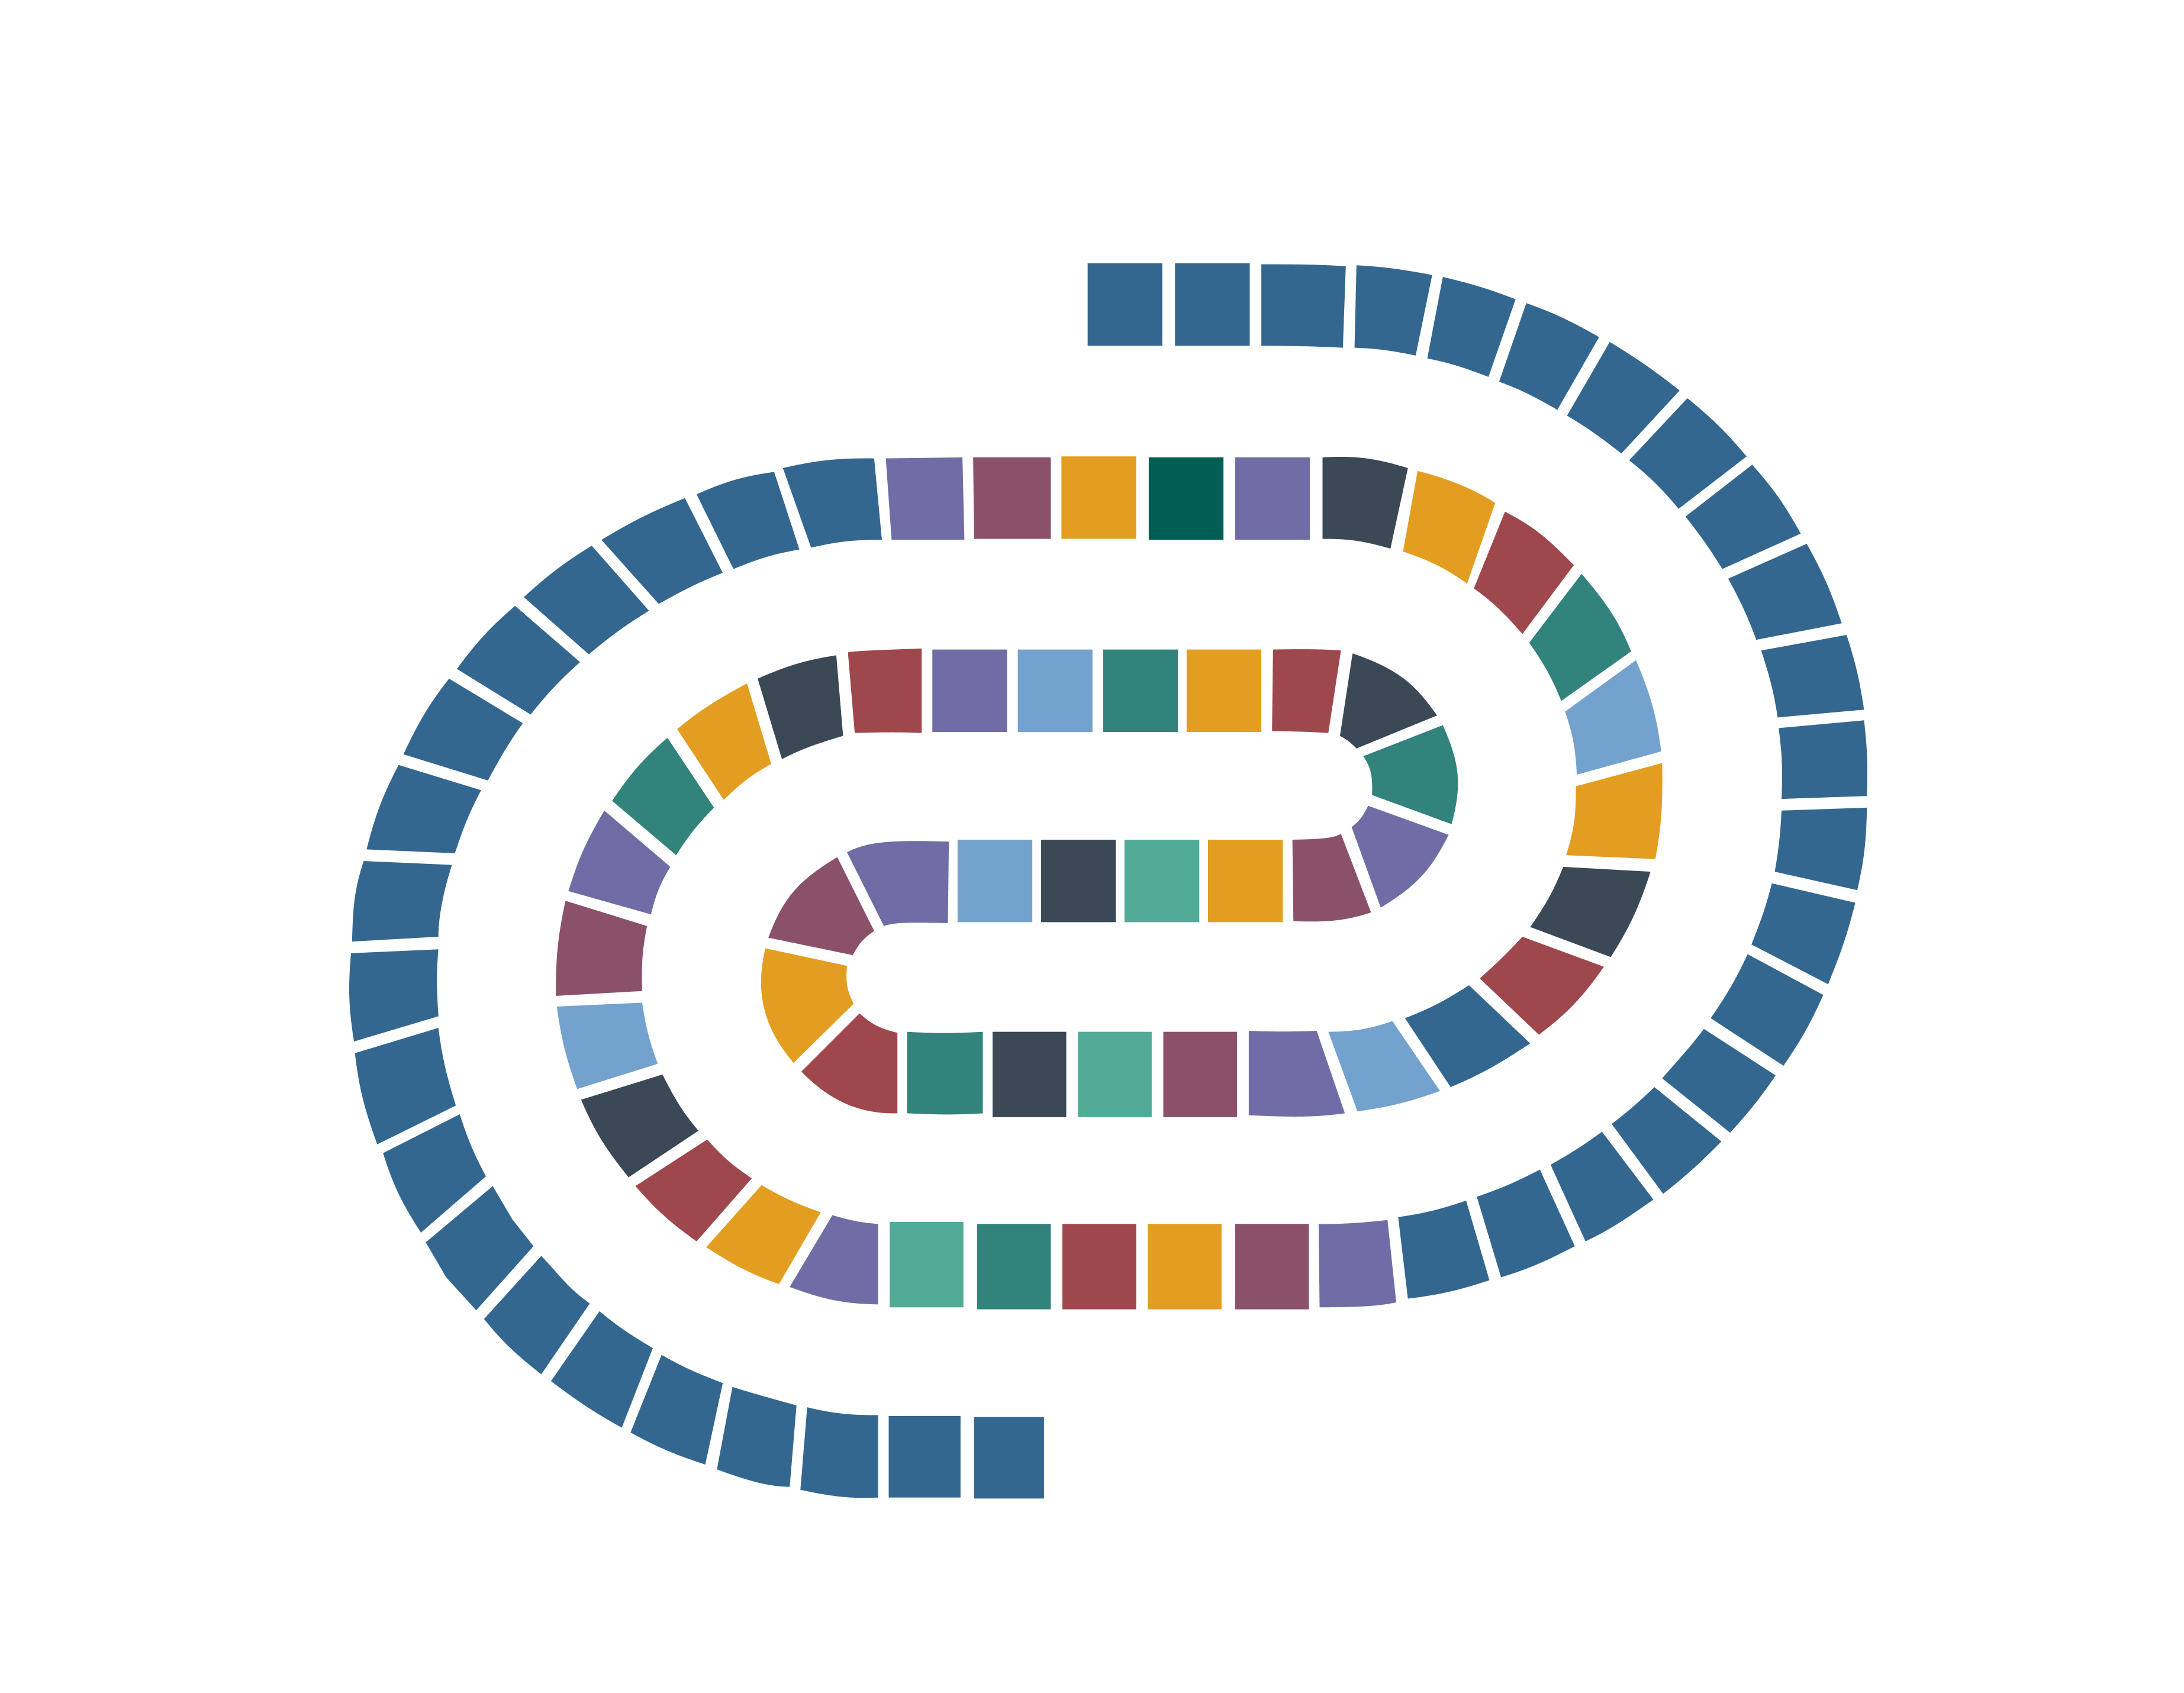
\includegraphics[width=12cm]{02_images/part_01/00_dasch_logo.png}
        \caption{Logo du \dsc}
    \end{figure}
    
        \subsection{Gouvernance du \dsc}
        
        Actuellement, l'\eng{Executive Board} du \dsc est dirigé par la Prof. Dr. \rg, qui occupe le poste de \eng{Head} du \eng{Repository Services}. Dr. Ivan Subotic est, quant à lui, le \eng{Deputy Director}. Les \eng{Repository Services}, dont Gautschy est la cheffe, englobent les départements de \eng{Product Management}, \eng{Interoperability and Archiving}. Concernant le \eng{Research Data Unit}, elle est également responsable du \eng{Research Data Management} et du \eng{Scientific Programming}. Ivan, en charge de l'\eng{Engineering}, s'occupe de l'\eng{Infrastructure}, du \eng{Software Development}, de l'\ux et du \eng{Support}.

        Par ailleurs, \rg est également l'interlocutrice principale pour d'autres partenariats du \dsc, tels que DARIAH-CH \footnote{Le consortium DARIAH-CH, constitué en novembre 2021, regroupe plusieurs institutions académiques suisses afin de favoriser la recherche et l'enseignement numériques dans le domaine des sciences humaines et sociales. Il vise à coordonner les activités liées à DARIAH en Suisse et à assurer une participation active du pays au sein de DARIAH-EU. Voir \cite{dariahch}.}, et l'\eng{Office Management}, lié à l'\unibas.

        % organigramme du \dsc
        \begin{figure}[h!]
            \centering
            \includegraphics[width=12cm]{02_images/part_01/02_executive_board.jpg}
            \caption{Organigramme du \dsc}
        \end{figure}

        % SI JAMAIS, CELA FONCTIONNE
        % \begin{figure}[htbp]
        %     \centering
        %         \savebox{\savefig}{\includegraphics[width=10cm, height=8cm]{02_images/02_executive_board.jpg}} 
        %     \rotatebox{90}{%
        %     \begin{minipage}{\wd\savefig}
        %         \usebox{\savefig}
        %         \caption{Swimlane Diagram}
        %     \end{minipage}}
        % \end{figure}

        Le \dsc adopte un modèle de gouvernance participative qui vise à englober l'ensemble des acteurs concernés par la recherche en sciences humaines en Suisse. Cette approche inclusive se traduit par une adhésion ouverte à un large éventail d'institutions, allant des universités aux académies et aux infrastructures de recherche spécialisées. Cette diversité de membres garantit une représentation équilibrée des différents domaines et perspectives de la recherche.

        Un autre aspect fondamental de la gouvernance du \dsc est son indépendance vis-à-vis de toute institution d'enseignement supérieur particulière. Cette autonomie permet d'éviter les conflits d'intérêts et d'assurer une prise de décisions objective et impartiale. En outre, l'indépendance du \dsc renforce sa crédibilité et sa légitimité en tant que plateforme neutre pour la recherche en sciences humaines.

        % gouvernance du Dasch
        \begin{figure}[h!]
            \centering
            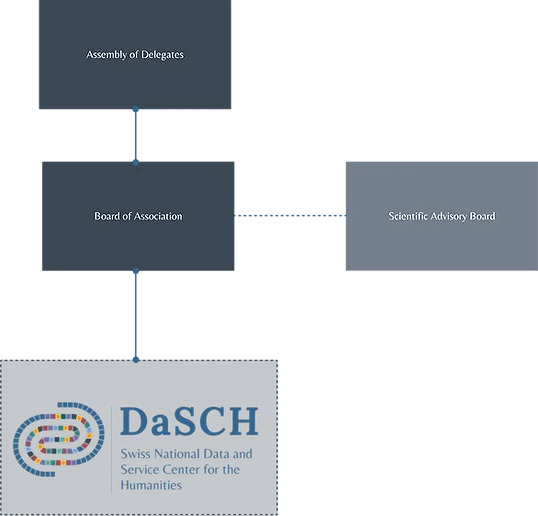
\includegraphics[width=12cm]{02_images/part_01/03_board_association.jpg}
            \caption{Gouvernance du \dsc}
        \end{figure}

        La gouvernance du \dsc est également caractérisée par son efficacité et son efficience. En limitant les formalités administratives, l'association peut se concentrer sur ses missions essentielles, telles que la mise à disposition de ressources et de services pour la recherche \footnote{Selon le site web du \dsc, l'association a \og{peu de formalités administratives}\fg. Voir \cite{gov_dasch}.}. Cette approche pragmatique permet d'optimiser l'utilisation des ressources et de garantir une réponse rapide aux besoins des chercheurs.

        La gouvernance participative et indépendante du \dsc est l'un des piliers de son fonctionnement. Pour comprendre comment cette organisation est parvenue à mettre en place une telle gouvernance efficace et inclusive, il est essentiel de revenir sur ses origines et les raisons de sa création.
    
        \subsection{Fondation du \dsc}
    
        Depuis sa création, \dsc est le fruit d'une initiative conjointe du \dhlab de l'\unibas et de la \sagw. Cette initiative a vu le jour dans le cadre d'un projet pilote ancré à \ERID 2013–2016.
    
        L'origine du \dsc remonte à un consortium réunissant les universités de Bâle, Berne et Lausanne, avec la direction assurée par le Digital Humanities Lab de l'\unibas. Ce consortium a remporté un appel d'offres public lancé par SAGW, marquant ainsi le début des efforts pour créer une infrastructure nationale dédiée aux données de recherche en sciences humaines. Pendant la phase pilote, une étude de faisabilité sur la solution technique choisie a été menée à bien, utilisant divers jeux de données.
    
        En 2017, le \dsc a été officiellement établi en tant qu'infrastructure nationale, opérée par SAGW, avec un mandat défini dans l'\erid 2017–2020. Cette reconnaissance institutionnelle a permis au \dsc de se structurer et de s'intégrer pleinement dans le paysage national de la recherche en sciences humaines, en apportant des solutions innovantes pour la gestion et la préservation des données de recherche.
        
        Depuis 2021, le \dsc fonctionne comme une infrastructure nationale de données de recherche, bénéficiant principalement d'un financement de la part du \SNSFn. Cette évolution témoigne de l'importance croissante des humanités numériques et de la reconnaissance de la nécessité de disposer de structures robustes et durables pour le archivage, l'accès et l'exploitation des données de recherche dans ce domaine.

        
        \begin{figure}[h!]
            \centering
            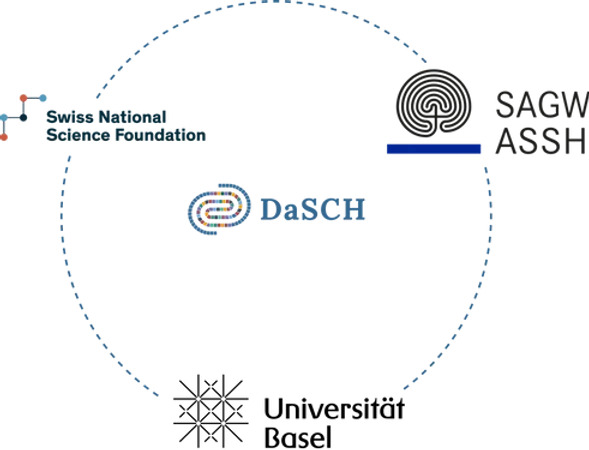
\includegraphics[width=12cm]{02_images/part_01/01_funding.jpg}
            \caption{Schéma de fonctionnement du \dsc}
        \end{figure}
    
        Ainsi, la fondation du \dsc illustre une réponse concertée aux besoins émergents des sciences humaines à l'ère du numérique, en mettant en place des infrastructures capables de soutenir les chercheurs dans leurs travaux et de valoriser les données produites par leurs recherches. Fort de ce socle, le \dsc a mis également en place une plateforme numérique qui va bien au-delà du simple archivage de données. Nous allons donc aborder par la suite comment fonctionne cette plateforme.

        
        \subsection{\dsc et l'\opdt en Suisse}

        \dsc possède une plateforme pour les données de recherche ouvertes dans les sciences humaines en Suisse. Cet environnement de recherche virtuel peut être utilisé tant pour ceux et celles qui veulent publier ces données quant pour ceux et celles qui veulent réutiliser ses données \footnote{Voir \cite{re3data}.}. C'est aussi important souligner que \dsc développe et exploite un dépôt à long terme conforme aux principes FAIR (\eng{Findable}, \eng{Accessible}, \eng{Interoperable}, \eng{Reusable}). Pour ces raison, nous pouvons voir que \dsc s’assure que les informations collectées soient non seulement accessibles et réutilisables par la communauté scientifique, mais aussi qu’elles respectent les normes internationales de gestion de données. Cela permet non seulement de préserver le patrimoine scientifique de manière durable, mais aussi de faciliter la collaboration et l’innovation au sein de la communauté académique.

        En deuxième place, l’environnement de recherche virtuel proposé par \dsc offre aux chercheurs une plateforme intégrée qui simplifie l’archivage, la gestion et le partage de leurs données. Cette infrastructure est essentielle pour promouvoir la transparence et l’efficacité dans les processus de recherche, en assurant que les données sont disponibles et exploitables à long terme. Cela va de soi avec l'idée de \psdn, une fois que ce processus d'archivage permet une identification de données.

        Néanmoins, l'archivage de données en soi n'assure pas une \psdn lors de l'interopérabilité. Pour montrer comment ces données sont interprétées et comprises, ainsi que la manière dont la communauté est intégrée, nous allons maintenant analyser les stratégies de \dsc.
        
        \subsection{Stratégies de \dsc}
        La stratégie de \dsc repose sur trois piliers fondamentaux, chacun jouant un rôle essentiel dans la réalisation de ses objectifs à court et long terme \footnote{Les trois pilliers mentionnés sont expliqués dans la partie \eng{Strategic Goals} sur le site. Voir \cite{daschstrategicgoals}.}. Le premier pilier, l'extension technique de la plateforme, est une réponse directe aux besoins croissants d'évolutivité et de flexibilité dans la gestion des données de recherche. En rendant la plateforme plus accessible et adaptable, \dsc vise à offrir aux chercheurs un outil performant et intuitif, tout en permettant l'intégration de nouvelles technologies. Cela ne se limite pas à l'amélioration de l'expérience utilisateur, mais s'étend également à l'augmentation de l'interopérabilité en encourageant l'adoption de standards reconnus et de données normées. Cette approche permet non seulement de faciliter la réutilisation des données, mais aussi d'assurer leur pérennité dans un environnement de recherche en constante évolution.
        
        Le deuxième pilier de la stratégie de \dsc est le soutien à la création de communauté et à l'éducation. \dsc reconnaît que la technologie seule ne suffit pas à garantir le succès de sa plateforme. En connectant les chercheurs entre eux et en leur offrant des opportunités de formation, \dsc renforce les liens au sein de la communauté scientifique. Cela inclut non seulement l'organisation d'événements pour échanger sur les besoins et les défis rencontrés, mais aussi l'offre de formations adaptées, en particulier pour les jeunes chercheurs. Cette orientation vers l'éducation et le soutien communautaire est cruciale pour garantir que la plateforme \dsc soit non seulement utilisée, mais aussi optimisée et améliorée grâce aux retours de ses utilisateurs, assurant ainsi une évolution en phase avec les besoins réels des chercheurs.
        
        Enfin, le troisième pilier consiste en un renforcement des réseaux et des coopérations, tant au niveau national qu'international. \dsc comprend que la collaboration est essentielle pour avancer dans la recherche et la gestion des données. En s'associant avec d'autres institutions et en participant activement à des projets internationaux, \dsc vise à créer des synergies qui permettent de développer des solutions innovantes pour l'accessibilité, l'interopérabilité et la conservation à long terme des données. L'engagement de \dsc dans des initiatives comme DARIAH et la définition de standards IIIF pour les images 3D témoigne de sa volonté de jouer un rôle de premier plan dans la normalisation et l'amélioration des pratiques de gestion des données de recherche. Cette stratégie de coopération est non seulement bénéfique pour \dsc, mais elle contribue également à l'avancement de la recherche en sciences humaines dans son ensemble.

        Le développement et le maintien d'une infrastructure et des stratégies aussi complexe que \dsc nécessitent des investissements conséquents et durables. Nous allons expliquer alors comment s'opère le financement de l'association.
        
        \subsection{Financement du \dsc}

        Concernant le financement du \dsc, l'association bénéficie d'un financement principal du SNSF, qui a octroyé un soutien significatif pour la période 2021 à 2024, intitulé \erid 2021-2024. Cet accord de financement a permis de définir clairement les services que le \dsc doit fournir à la communauté scientifique suisse. En plus de ce financement public, l'\unibas apporte des contributions en nature, telles que l'hébergement de l'infrastructure et la mise à disposition de ressources humaines.

        Ces ressources financières permettent au \dsc de développer et de maintenir une infrastructure numérique. Cependant, pour étendre ses services et répondre à des demandes spécifiques, le \dsc peut également solliciter des financements supplémentaires auprès de tiers ou des utilisateurs eux-mêmes. Ces contributions peuvent prendre la forme de partenariats, de projets de recherche ou de frais d'utilisation de certains services.

        Nous allons maintenant nous pencher plus en détail sur l'\erid pour comprendre comment il fonctionne et pourquoi il est important pour comprendre les enjeux du \dsc dans ce contexte de \psdn.

            \subsubsection{Fonctionnement de l'\erid}
            Le système politique fédéral suisse considère que les investissements dans l'éducation, la recherche et l'innovation sont essentiels pour le succès du pays. C'est pourquoi des investissements sont réalisés dans ces domaines, car il est estimé que l'éducation et la recherche sont les fondements de la créativité et de l'entrepreneuriat. Ces éléments sont également des prérequis pour la capacité d'innovation et la compétitivité des entreprises suisses. Afin de soutenir les initiatives dans ces trois domaines, la Confédération suisse et les cantons financent et régulent le secteur de l'ERI par le biais du plan \ERID, accordé tous les quatre ans, afin de promouvoir ces initiatives \footnote{Le caractère cyclique des évaluations ERI peut conduire à des fluctuations dans l'importance accordée aux indicateurs DaSCH, ce qui peut créer une certaine instabilité dans les politiques publiques associées.}.
    
            Il est important de noter que le plan \erid est soumis à l'Assemblée fédérale avant d'être approuvé. Pour la période 2021-2024, à laquelle \dsc est associé, un investissement de 28,1 milliards de \textsc{chf} a été prévu, soit plus de 2 millions de \textsc{chf} par rapport au plan \ERID 2017-2020, qui est à l'origine de \dsc\footnote{Voir \cite{sbfi}.}.

            \begin{figure}[h!]
                \centering
                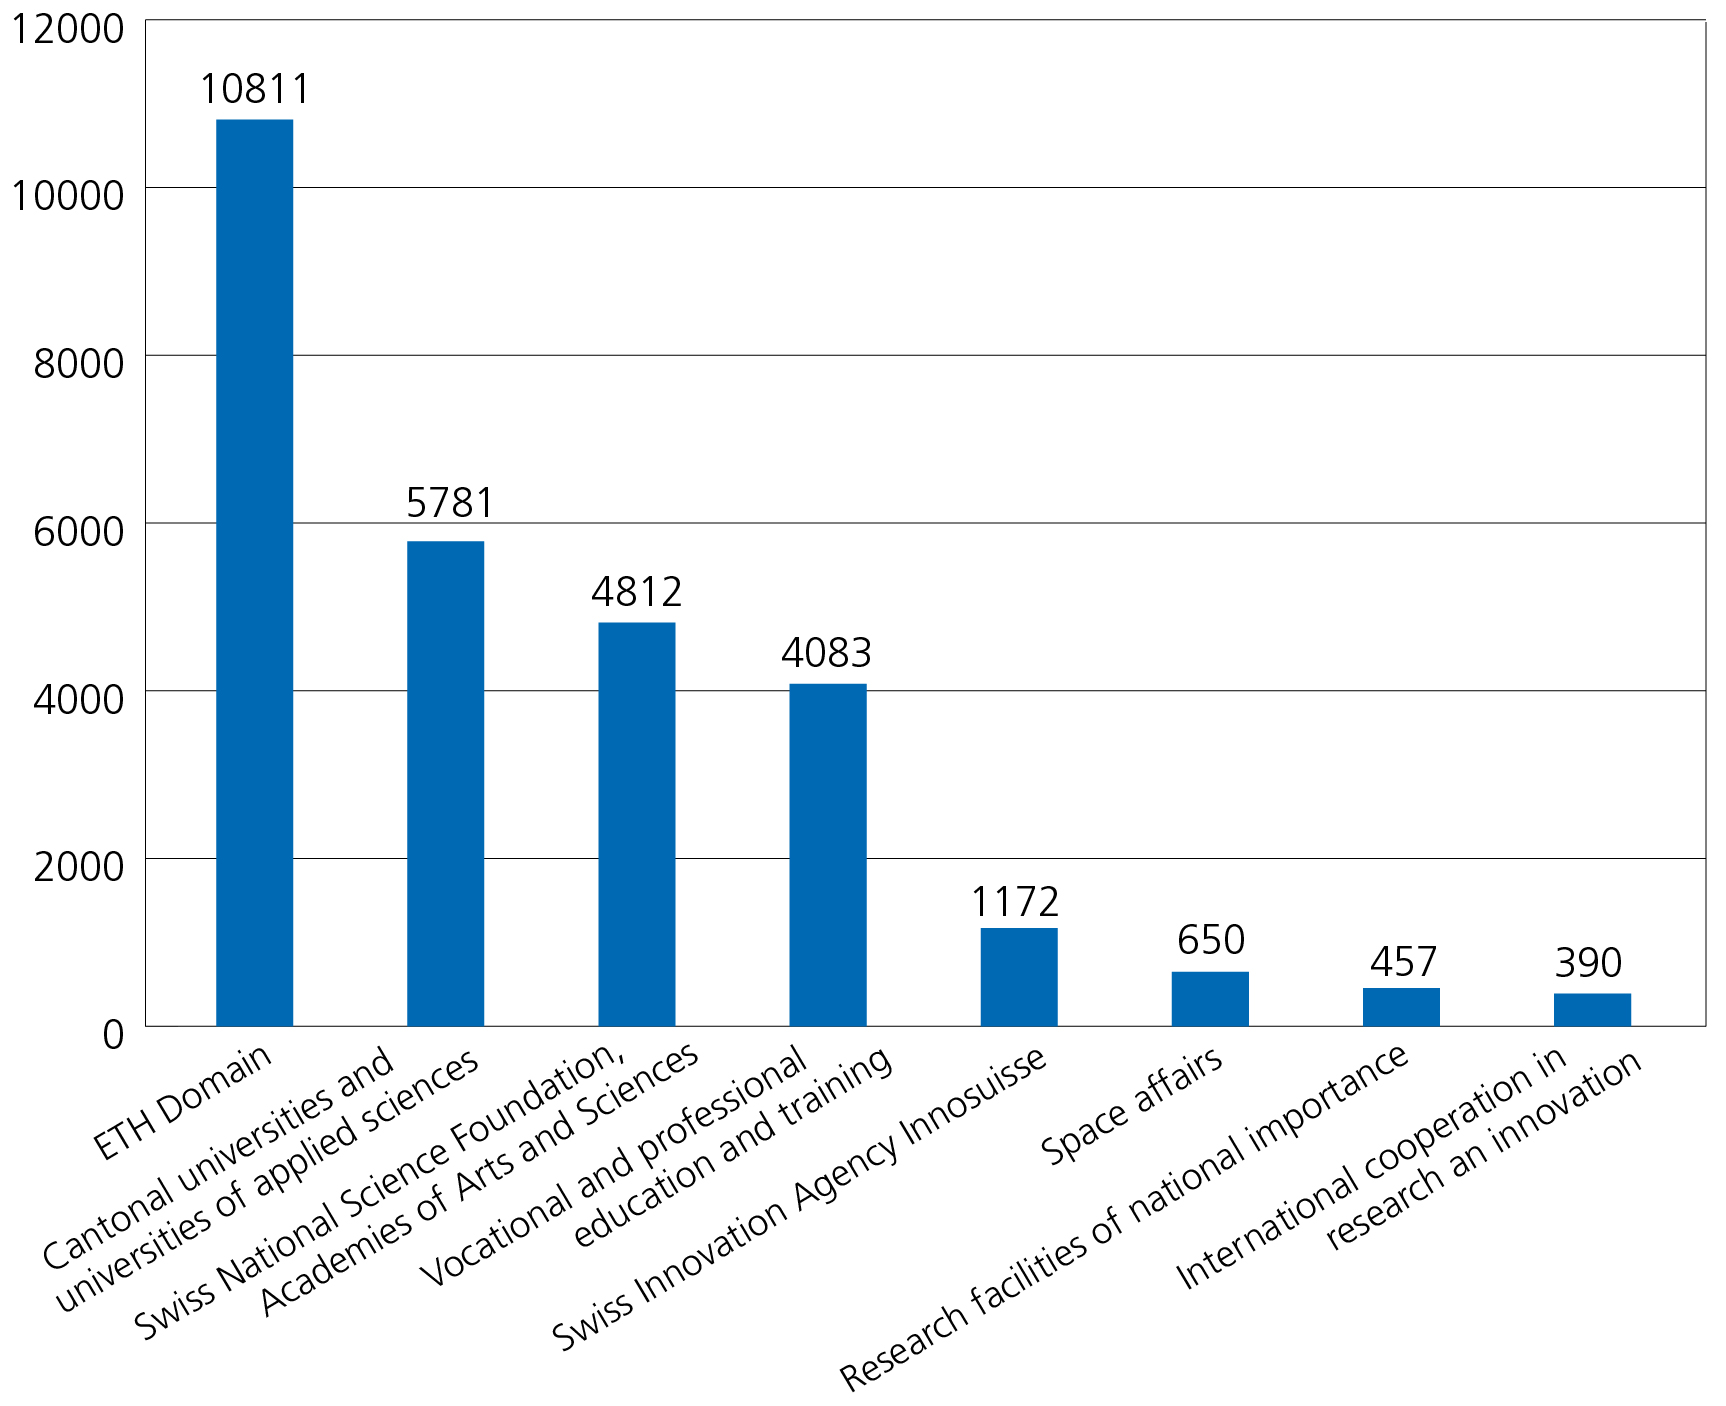
\includegraphics[width=12cm]{02_images/part_01/04_investissemnt_eri_2021_2024.jpg}
                \caption{Financement \erid alloué par l'Assemblée fédérale suisse pour 2021-2024, en millions. \textbf{Source} : \cite{sbfi}.}
            \end{figure}
    
            Enfin, il est également crucial de souligner que pour la période 2021-2024, les politiques du plan \ERID se concentrent sur trois thèmes principaux : la numérisation, le développement durable et l'égalité des chances. Ces politiques bénéficient de l'engagement des cantons et de tous les parties prenantes concernées\footnote{Voir \cite{sbfi}.}.

        
        \subsection{Notes conclusives}
        
        En conclusion, \dsc joue un rôle crucial dans la transformation numérique des sciences humaines en Suisse, en fournissant les outils et les services nécessaires pour une gestion optimale des données de recherche ouvertes, tout en respectant les plus hauts standards de qualité et de durabilité. Nous avons également constaté que pour \dsc, le standard IIIF occupe une place centrale dans ses préoccupations en matière de maintien de la persistance des données. C'est pourquoi nous allons maintenant nous pencher sur ce qu'est le standard IIIF, afin de comprendre l'importance qu'il a revêtue lors de la mise en œuvre des \eng{pipelines} au cours de mon stage.


\chapter{Contexte IIIF}

    \section{Qu'est-ce que l'IIIF ?}
    
    Le standard \iiif est un ensemble de normes ouvertes conçues pour la gestion des objets numériques. Soutenues par une communauté internationale, les APIs IIIF constituent un élément fondamental en permettant l'ajout d'informations descriptives aux objets numériques. Cela assure non seulement que ces informations soient accessibles et compréhensibles pour les utilisateurs humains (\textit{human readable}), mais facilite également l'affichage des images. De plus, la communauté IIIF s'efforce constamment de maintenir et d'améliorer ces APIs, garantissant ainsi leur compatibilité avec une large variété d'objets 2D. De plus, avec l'introduction de la version 4.0, des discussions sont en cours pour étendre ce support aux modèles 3D, ouvrant ainsi de nouvelles perspectives dans la gestion des ressources numériques.
    
    Avant de nous plonger plus profondément dans les aspects techniques de l'API 3.0, il est pertinent de comprendre l'histoire de son développement, ce qui nous permet de mieux saisir les enjeux actuels et les futures évolutions envisagées par la communauté.

    \section{Origines d'IIIF}
    
    L'origine d'IIIF daterait environ du début des années 2010, à partir d'une discussion informelle entre technologistes de \eng{Stanford University}, \eng{Oxford University} et de la \eng{British Library} dans un café, et, par la suite, différentes bibliothèques nationales et internationales ont rejoint l'initiative \footnote{Les deux versions sont d'accord sur les années du début, néanmoins c'est la thèse de Raemy qui raconte qui étaient les acteurs principaux et les institutions lors de la création d'IIIF. Pour les deux versions, voir la thèse de Raemy \cite[p.~13]{raemy2017iiif} et le site de Biblissima, Voir \cite{biblissima_iiif_intro}}. IIIF est actuellement un \textit{consortium} international qui rassemble différentes organisations du monde et qui a également une communauté de musées, archives, bibliothèques, instituts de recherche, sociétés de services informatiques qui entretiennent les APIs IIIF.

    La communauté IIIF a pour mission de définir, de diffuser et de faire évoluer les normes techniques IIIF en s'appuyant sur des cas d'usage concrets. C'est dans cette perspective que l'ambition de IIIF est de créer un cadre technique commun, permettant aux fournisseurs de ressources numériques de délivrer leurs contenus de manière standardisée sur le Web, afin de les rendre consultables, manipulables et annotables par n'importe quel logiciel compatible \footnote{Voir \cite{biblissima_iiif_intro}}.

    % schéma IIIF
        \begin{figure}[h!]
            \centering
            \includegraphics[width=12cm]{02_images/part_01/09_schema_iiif.png}
            \caption{Schéma : principe général d’interopérabilité de IIIF (trois applications différentes sont branchées à trois entrepôts IIIF).}
        \end{figure}
     
    \section{Intégration d'IIIF pour la valorisation du patrimoine}
    
    Le standard IIIF (International Image Interoperability Framework) s'est imposé comme un outil incontournable pour l'archivage et la diffusion d'objets numériques au sein des institutions patrimoniales. En associant un objet numérique à un fichier \textsc{json}, ce standard offre une méthode simple et flexible pour décrire et rendre accessible un large éventail de ressources.

    Dans un premier temps, il est essentiel de souligner l'adoption généralisée du IIIF par de nombreuses institutions culturelles de renommée mondiale, telles que la Bibliothèque nationale de France ou les Musées du Vatican. Cette adhésion massive témoigne de l'efficacité du standard pour répondre aux besoins spécifiques des institutions patrimoniales, en particulier en matière de préservation et de valorisation des collections.
    
    Ensuite, la popularité du IIIF s'explique par sa capacité à rendre les objets numériques et leurs métadonnées accessibles à un large public grâce à des \eng{viewers} en ligne, qui sont des outils pour rendre les modèles 3D visibles sur le web, tels Mirador, Universal Viewer et OpenSeadragon \footnote{Mirador, Universal et OpenSeadragon sont trois projects \opso qui permettent de visualiser ces modèles 3D. Pour plus de détails sur ces viewers, Voir \cite{mirador}, \cite{universalviewer} et \cite{openseadragon}}. Ces outils permettent également d'explorer les collections de manière interactive, de réaliser des comparaisons, d'annoter les images et voire de zoomer en haute définition \footnote{Alors que le texte de Rossenova vise un large public, il faut souligner que les \eng{viewers} permettent ces autres possibilités. Voir \cite{rossenova2023iiif}.}. Cette dimension visuelle est particulièrement appréciée des chercheurs et du grand public, qui peuvent ainsi bénéficier d'une expérience utilisateur enrichie. Voyons un exemple avec Mirador \footnote{Pour regarder la démonstration de Mirador, Voir \cite{mirador_demo}.} :

    % Mirador : comparaison
        \begin{figure}[h!]
            \centering
            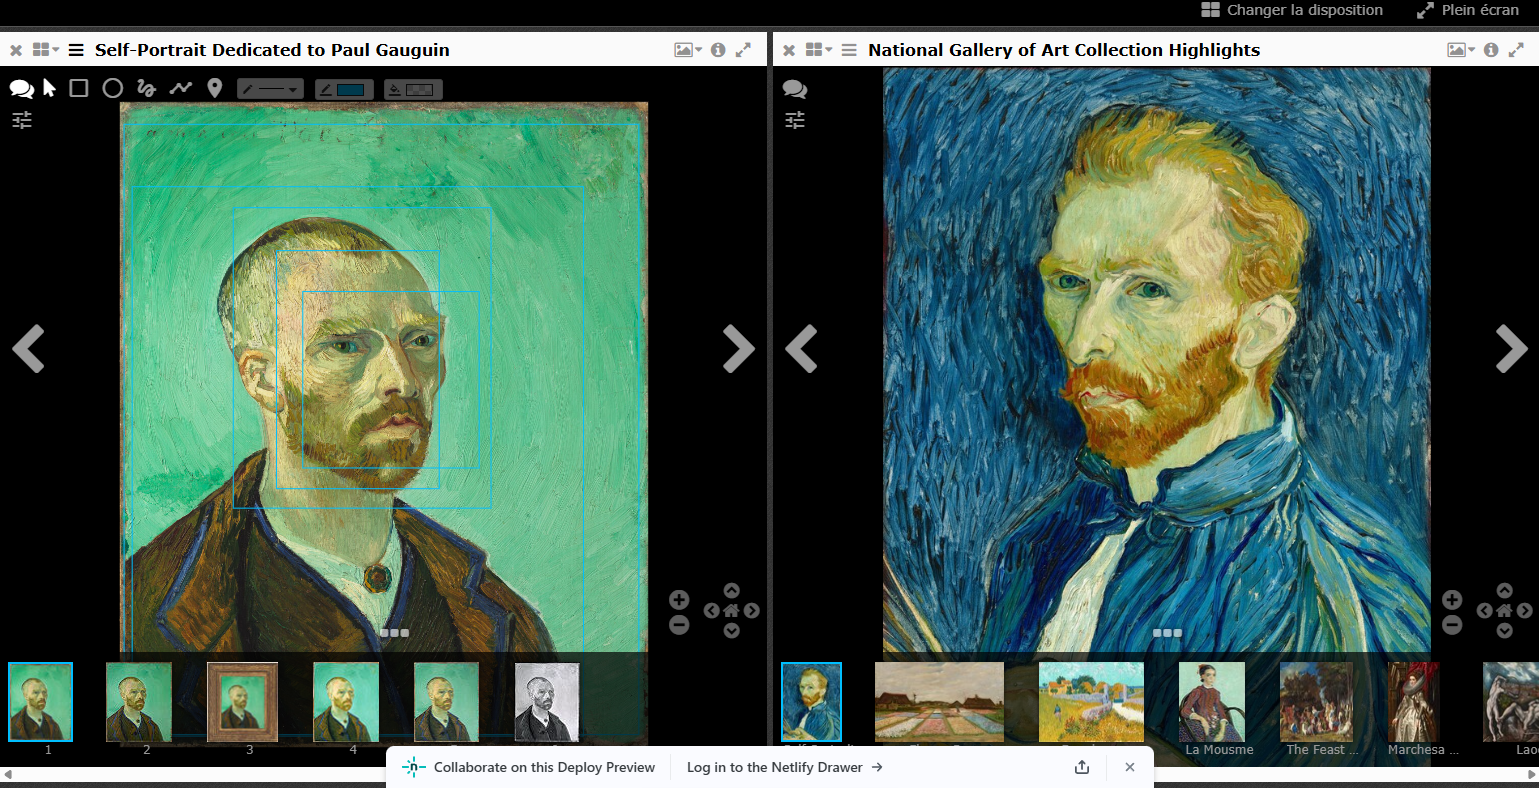
\includegraphics[width=12cm]{02_images/part_01/11_mirador_01.png}
            \caption{Mirador: comparaison entre images de différentes institutions.}
        \end{figure}

    % Mirador : exemple d'annotation
        \begin{figure}[h!]
            \centering
            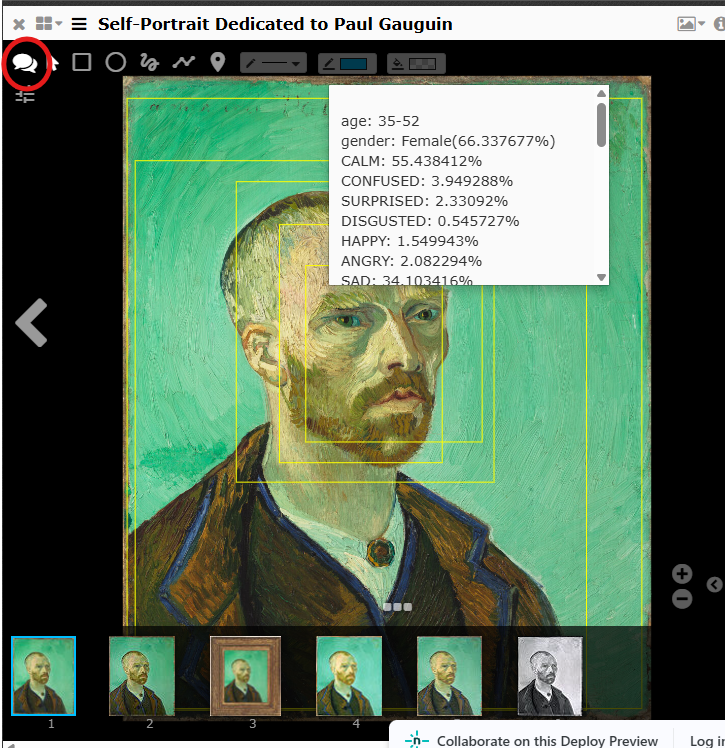
\includegraphics[width=12cm]{02_images/part_01/12_mirador_02.png}
            \caption{Mirador: exemple d'image annotée, avec l'outil d'annotations du \eng{viewer}.}
        \end{figure}

    % Mirador : zoom en haute définition de l'image de Van Gogh
        \begin{figure}[h!]
            \centering
            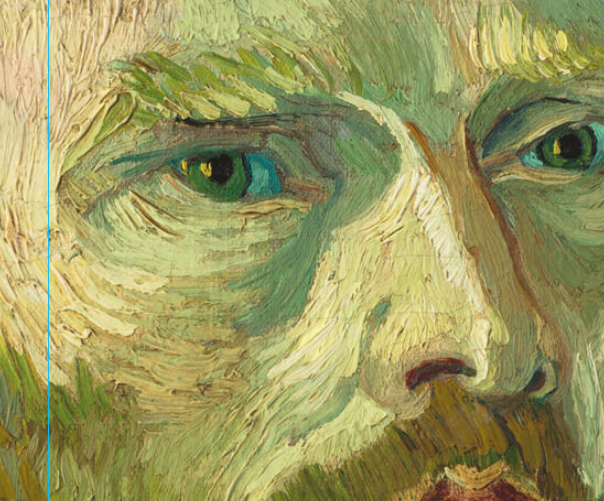
\includegraphics[width=12cm]{02_images/part_01/13_mirador_03.png}
            \caption{Mirador : zoom en haute définition dans un détail de la première image.}
        \end{figure}
    
    Par ailleurs, le IIIF offre une grande flexibilité dans la structuration des données. Il est ainsi possible d'archiver des objets avec un minimum d'informations, ce qui facilite l'intégration rapide de nouvelles acquisitions dans les collections. De plus, le standard permet de décrire des objets complexes et de gérer des ensembles d'images multiples, favorisant ainsi une approche holistique de l'archivage.
    
    En outre, le IIIF joue un rôle essentiel dans la diffusion d'images haute résolution. En réduisant les contraintes liées au stockage et à la bande passante, il permet de partager des images de grande qualité sans compromettre les performances. Cette caractéristique est particulièrement intéressante pour les institutions qui souhaitent mettre à disposition du public des reproductions numériques de haute fidélité de leurs œuvres.
    
    Enfin, l'une des forces du IIIF réside dans sa capacité à favoriser l'interopérabilité entre les différentes institutions. Grâce aux manifestes IIIF, il est possible de créer des liens entre des objets provenant de sources diverses et de construire des narrations entre eux. Cette fonctionnalité ouvre de nouvelles perspectives pour la recherche et la collaboration entre les institutions culturelles.
    
    En conclusion, le standard IIIF constitue une solution efficace et flexible pour l'archivage et la diffusion d'objets numériques. En offrant une structure simple et ouverte, il permet aux institutions patrimoniales de préserver leur patrimoine et de le rendre accessible à un public toujours plus large. Cependant, l'exploitation optimale du IIIF nécessite une réflexion approfondie sur les enjeux liés à la gestion des données, à l'interopérabilité et à la pérennité des infrastructures numériques.

    \section{IIIF API 3.0.}
    
    L'importance d'expliquer l'API 3.0 réside dans le fait qu'elle est la plus utilisée par les institutions travaillant dans le domaine patrimonial. De plus, elle constitue la base pour la conception de l'API 4.0. Il est donc fondamental de bien comprendre les principes de l'API 3.0 pour saisir non seulement son importance actuelle, mais aussi les raisons pour lesquelles elle a été essentielle dans le cadre de mon stage.
    
    L'API IIIF 3.0 se compose de quatre API RESTful au format JSON-LD : Image API, Presentation API, Content Search API et Authentification API. Pour bien comprendre chacune de ces API dans notre étude, nous allons en expliquer le fonctionnement et analyser ensuite les enjeux pour \dsc avec les applications développées durant le stage, ce qui nous aidera à comprendre l'importance future de l'API 4.0 pour notre travail.
    

    \subsubsection{Image API}
    
    La première version de l'\iapit a été lancée en août 2012 \footnote{Voir Pour ces prochains chapitres, nous avons suivi l'ordre chronologique explicatif suggéré par les travaux de Julien Raemy. Voir \cite{raemy2017iiif}} et la fonction basique de cette API est de prendre les données techniques d'une image et ses informations associées, pour les rendre visibles sur le web \footnote{Tous les concepts du chapitre ont été extraits et analysés à partir de la partie dédiee au \iapit sur le site d'IIIF. Voir \cite{iiifimage30}.}. Pour ce faire, elle requiert une URI définie selon une syntaxe stricte (Voir Tableau 2.1) \footnote{L'exemple de syntaxe a été extrait de la section d'Image API sur le site d'IIIF. Voir \cite{iiifimage30} En ce qui concerne l'idée de faire un tableau avec les requêtes, ce travail s'est inspiré de la suggestion de Raemy. Voir \cite[p.~20]{raemy2017iiif}.}.
    
        \begin{table}[h!]
        \centering
        \caption{Structure des requêtes d'image et d'information}
        \resizebox{\textwidth}{!}{
                \begin{tabular}{|l|l|}
                \hline
                \rowcolor{gray!20} % première ligne grise
                \textbf{Type de Requête}        & \textbf{Structure de la Requête}                                                                                      \\ \hline
                \textbf{Image Request}          & \{scheme\}://\{server\}\{/prefix\}/\{identifier\}/\{region\}/\{size\}/\{rotation\}/\{quality\}.\{format\}              \\ \hline
                \textbf{Exemple Image Request}  & \texttt{http://www.example.org/image-service/abcd1234/full/full/0/default.jpg}                                       \\ \hline
                \textbf{Image Information Request} & \{scheme\}://\{server\}\{/prefix\}/\{identifier\}/info.json                                                        \\ \hline
                \textbf{Exemple Information Request} & \texttt{http://www.example.org/image-service/abcd1234/info.json}                                                   \\ \hline
                \end{tabular}
            }
        \end{table}

    
    Comme nous pouvons le constater, les informations sont prises dans l'ordre indiqué dans le tableau. Il est important de mentionner que l'API ne pose aucune restriction quant à la forme des identifiants qu'un serveur peut utiliser ou prendre en charge, ce qui offre une grande flexibilité, même dans la conception des identifiants.
    
    L'image renvoyée est toujours la représentation de l'URI, ce qui signifie que l'URI peut modifier la nature de l'image affichée. Cela est crucial pour certaines institutions, car des paramètres comme la taille en \eng{pixels}, la couleur, ou d'autres aspects peuvent être ajustés en fonction des besoins spécifiques.
    
    \subsubsection{Presentation API}
    
    Le \eng{Presentation API} travaille avec des objets numérisés ou nativement numériques et son objectif principal est de fournir les informations nécessaires pour permettre une visualisation riche en ligne des objets numériques composés, souvent en combinaison avec l'\iapit \footnote{Tous les concepts du chapitre ont été extraits et analysés à partir de la partie dédiée au \papit sur le site d'IIIF. Les sources seront citées à chaque fois que cela sera nécessaire pour garantir la clarté sur les références. Voir \cite{iiifpresentation30}.}. Ces objets sont standardisés suivant une description en format \textsc{json}. Un objet dit composé peut être une série de pages, de surfaces, etc. Par exemple, il peut s'agir des deux faces d'une photographie, des quatre vues cardinales d'une statue, de papyrus, etc. Toutes ces spécifications suivent les principes du Linked Data et de l'architecture du Web pour garantir leur interopérabilité. De plus, le modèle de données Shared Canvas et \textsc{json-ld} permet de créer un format \textsc{json} facile à mettre en œuvre.
    
    Pour bien comprendre le fonctionnement du \eng{Presentation API} d'IIIF, il est essentiel de savoir comment les types de ressources sont classés dans la spécification des objets composés. Le modèle est structuré de la manière suivante : Collection, Manifest, Canvas et Range \footnote{Voir \cite{iiifpresentation30}}.
    
    Premièrement, une Collection est une liste ordonnée de Manifests et/ou d'autres Collections. Les Collections permettent de regrouper des Manifests et d'autres Collections dans une structure hiérarchique pour la présentation. Cette présentation peut être utilisée pour naviguer, afficher des résultats de recherche dynamiques ou fournir un ensemble de ressources fixes, quel que soit l'objectif \footnote{Voir \cite{iiifpresentation30}}.
    
    Deuxièmement, le Manifest décrit la structure et les propriétés d'un objet composé. Il contient les informations nécessaires pour qu'un client puisse afficher le contenu à un utilisateur, tels que le titre, les annotations ou les éléments intellectuels pertinents à l'objet. Bien qu’un Manifest peut représenter un seul objet (une image, donc), il est courant qu'un Manifest décrive un seul objet composé, comme un livre, un album musical, un objet archéologique, etc \footnote{Voir \cite{iiifpresentation30}}.
    
    Troisièmement, le Canvas est un espace virtuel, une sorte de conteneur, dont la fonction est de représenter une vue particulière d'un objet, associée à des ressources de contenu ou à des parties de celui-ci. Le Canvas sert principalement de référence pour la mise en page du contenu, tant sur le plan spatial que temporel. Le concept de Canvas est dérivé de normes telles que \textsc{pdf} et \html, ainsi que de logiciels comme \textsc{photoshop} et \textsc{powerpoint}, où une surface de départ accueille des images, des vidéos, du texte et d'autres contenus \enquote{peints} par annotations, rassemblés dans des pages d'annotation. Les annotations peuvent être affichées ou non, et cette archive associée peut varier, ce qui signifie qu'un même objet composé peut avoir plusieurs Canvas pour le représenter \footnote{Voir \cite{iiifpresentation30}}.
    
    Finalement, un Range est une liste ordonnée de Canvas et/ou d’autres Ranges. Les Ranges permettent de regrouper des Canvas, ou des sections de celles-ci, de manière structurée. Cela peut être motivé par des raisons liées au contenu, comme celles présentées dans une table des matières ou dans la succession des scènes d'une pièce de théâtre. De même, des caractéristiques physiques peuvent jouer un rôle important, par exemple la compilation de pages dans un livre, ou lorsque de la musique enregistrée est répartie sur différents supports physiques, tels que deux CD \footnote{Voir \cite{iiifpresentation30}}.

    \section{Vers l'IIIF API 4.0}
    
    Actuellement, la communauté IIIF développe le \papiq afin de gérer les modèles 3D \footnote{Toutes les discussions sur le développement de l'API peuvent être trouvées sur le GitHub de l'\eng{International Image Interoperability Framework}. Voir \cite{iiif3d}. Pour plus de détails sur le groupe, les buts et l'organisation, Voir \cite{iiif3dtsg}.}. Cette importance croissante provient du fait que les collections numériques, de plus en plus nombreuses, nécessitent non seulement des traitements spécifiques pour gérer leur capacité d'archivage et de rendu, mais aussi parce que d'autres types d'objets gagnent en importance dans le contexte de la recherche. Au-delà des œuvres d'art et des collection naturalistes, les objets archéologiques, les plans de sites et même les modèles 3D d'architectures historiques gagnent en importance dans le contexte de la recherche, comme c'était le cas chez \dsc.

    De plus, le contexte de production des objets est mis en évidence lors de leur numérisation. C'est pourquoi le \papiq a été conçu pour répondre à ces nouvelles demandes et proposer de nouvelles façons de valoriser les archives. Cela se remarque déjà à partir du remplacement d'un concept clé pour le \papit : nous parlons dorénavant de \enquote{Scene}, pas de \enquote{Canvas} ; le fichier \textsc{json} qui définissait les fichiers comme \enquote{Canvas}, maintenant définit les objets comme une seule \enquote{Scene} ou un ensemble de \enquote{Scenes}. Ces paramètres minimaux explicités par les développeurs, comme Julie Winchester \footnote{Julie Winchester est la Directrice technique (\eng{Technical director}) pour MorphoSource, un dépôt pour les \eng{scans} 3D d'échantillons biologiques et d'autres objets physiques, et a été nommée l'éditrice de spécifications (\eng{specification Editor}) d'IIIF en janvier 2024 \cite{iiifjulie2024}.}, sont documentés et on les abordera lors de l'explication du code \diiif.

    En outre, de nouvelles options de description ont été ajoutées, permettant au \papiq de proposer de nouvelles interactions avec les objets, comme par exemple les caméras et les lumières, qui changent le comportement des objets lors de l'affichage sur des \eng{viewers} \footnote{Les \enquote{Scenes} offrent aussi des dimensions infinies (X, Y, Z ou polaires), une origine centrale et permettent d'intégrer divers éléments (images, modèles 3D, etc.), \cite[p.~64]{ioannides_patias_2023}.}.

    C'est donc dans ce contexte de création de nouvelles formes de valorisation du patrimoine et de recherche de solutions adaptées à ces nouveaux besoins que \dsc s'intéresse à répondre, en priorité, aux besoins de la communauté travaillant avec ces différents objets, mais aussi à envisager des stratégies pour s'adapter au futur API 4.0. Quelles informations sont pertinentes ? Ce sont des questions qui seront analysées dans le quatrième chapitre de ce travail. Avant de procéder à cette analyse, nous avons encore besoin de quelques définitions théoriques fondamentales pour mieux comprendre le problème auquel \dsc est confronté.

\chapter{Persistance des données}

La manière dont nous concevons et représentons les données est fondamentale. Les normes et standards, souvent sources de débats terminologiques, influencent directement notre capacité à préserver et à diffuser les données. Ce chapitre explorera les différentes notions utilisées pour définir les "choses" que nous représentons en données numériques ou sont déjà nées numériques, et les implications de ces choix sur la manière dont nous les codons et les conservons. Cette réflexion vise également à repenser la notion de durabilité des données. 
    
        \section{Document, artefact et données}
        
        Bien qu'il soit vrai, comme le soulignait Marc Bloch, qu'un seul document ne suffit pas à faire l'histoire \footnote{\cite[p.~37-42]{bloch1952}.}, il est tout aussi exact d'affirmer, avec Langlois et Seignobos, que sans document, il n'y a pas d'histoire \footnote{\cite[p.~13]{langlois_seignobos1992}}. Ces deux affirmations révèlent la nature intrinsèquement historique des documents, quels qu'ils soient. De plus, les documents, outre leur diversité, s'inscrivent pleinement dans la culture matérielle, au même titre que les objets. Pour mieux comprendre ces implications, il convient de réviser la définition traditionnelle de document.

        Lors d'une conférence, l'archéologue Ulpiano Meneses nous rappelle que le terme \enquote{document} vient de la même racine du mot latin \textit{doceo}, qui signifie enseigner. Or, enseigner implique la transmission d'un savoir établi, ce qui fait du mot \textit{documentum} un modèle, un paradigme préétabli \footnote{\cite[p.~1-3]{meneses1980}.}. Cependant, Ulpiano nous met en garde contre cette conception trop restrictive du document comme simple source d'information \footnote{Un travail sur la philosophie de l'information que serait intéressant d'aborder dans un étude futur, c'est la formulation de la théorie sémantique de l'information sémantique de Floridi. Voir Chapitre 4 e Chapitre 5 \cite{floridi_2011}.}.

        Ainsi, pour dépasser cette vision, nous devons élargir la notion de document au-delà de la simple idée d' \enquote{enregistrer et conserver une information}. En effet, si nous nous limitons à cette définition, nous risquons de réduire le document à un texte écrit. Or, un document peut également être une source orale, mais aussi un objet. Cette idée, bien qu'elle ne soit pas nouvelle, mérite d'être rediscutée parce qu'elle met en lumière le fait que les conceptualisations peuvent être assez floues pour un document : les documents dont la nature n'est pas nécessairement d'être conservés, comme les lettres \footnote{\cite[p.~2]{meneses1980}.}, ou encore, comme mentionné, la restriction de source écrite à la notion de document. Selon Meneses, les artefacts, tout ce qui est produit par l'action humaine, sont l'un des principaux composants de la culture matérielle, voire des produits et des vecteurs de relations sociales. Selon l'auteur, ils sont à la fois issus de modes d'organisation sociale spécifiques et historiquement déterminés, et orientent et facilitent les relations sociales dans certaines directions \footnote{\cite[p.~112-113]{meneses1983}.}.
     
        Par ailleurs, il est essentiel de prendre en compte la dimension temporelle inhérente non seulement aux documents, mais aussi à leur conservation. En effet, un même document peut contenir des temporalités différentes, c'est-à-dire des traces de différentes époques. Comme le rappelle Ulpiano en citant Radley, \enquote{artefacts survive in ways unintended by makers and owners} \footnote{La phrase peut être traduite comme \enquote{les artefacts survivent d'une manière que leurs créateurs et leurs propriétaires n'avaient pas prévue}. \cite[p.~90.]{meneses1998}}. La numérisation de ces documents n'est donc pas une simple opération technique de conservation, mais un véritable travail de mémoire. Ce travail consiste à rendre compte des différentes strates temporelles contenues dans un document et à en tirer des informations sur les dynamiques sociales. La manière dont nous conservons un document aujourd'hui nous renseigne peut-être moins sur la société qui l'a produit.
    
        Enfin, comme le souligne le poète brésilien Carlos Drummond de Andrade dans son poème \textit{A Suposta existêcia}, \enquote{Les choses existent-elles/si elles ne sont pas vues ?} \footnote{\cite[p.~1]{meneses1980}.}. Ainsi, nous devons nous interroger sur ce que nous choisissons de conserver. En effet, la sélection historique des documents à numériser implique une prise de position qui reflète notre conception de ce qui est important de transmettre, de documenter.

        Ainsi, la culture matérielle nous sert à penser la notion de document et, par conséquent, de donnée. 
        
        \section{Culture matérielle et la \psdn}
        D’après Krzysztof Pomian, étudier l’histoire des musées permet comprendre les sociétés dans lesquelles s’est inscrite cette institution \footnote{\cite[p.~18]{pomian2020}.}. Cet argument est aussi éloquent en ce qui concerne la production des données numériques, étant donné que produire des données est aussi une forme de collectionner au sens premier du mot, de collecte. Étudier la formation d'une collection renvoie non seulement à la compréhension de l’origine d'une institution, y compris dans le système de pensée déjà crée dans lequel l’objet s’inscrit, mais aussi des \enquote{choses} dans un contexte historique précis.

        Réfléchir comme nous concevons une collection peut constituer une source historique de la culture matérielle. Pour discuter la notion que nous intéresse, il est important de dire que la construction de cette théorie a été faite de différentes manières par le monde, sans suivre un programme strict. À partir de l’ouvrage \textit{The socialness of things: essays on the socio-semiotics of objects} (1994) de Stephen H. Riggins, Daniel Miller a déjà souligné que les études à propos des \enquote{formes culturelle} sont issues des \enquote{analyses structurales et sémiotiques} dont les principales références étaient Roland Barthes, Jean Baudrillard, Mary Douglas et Claude Lévi-Strauss, aussi que Le système des objets (1968), écrit par Jean Baudrillard, a été une référence essentielle pour l’élaboration de la notion de culture matérielle dans la sémiologie \footnote{Voir \cite{martin1996, miller1988, moxey2008, rede2001}.}.

        La notion de culture matérielle qui nous intéresse vient, d’abord, de la théorie de la circulation des objets chez Igor Kopytoff. En fait, le principe selon lequel la marchandisation des choses n’est qu’une phase dans la biographie des choses \footnote{\cite[p.~83]{kopytoff1986}.}, présupposé soutenu aussi par Appadurai dans l’article « Introduction : commodities and the politics of value »\footnote{\cite[p.~16-17]{appadurai1986}.}, est fondamental pour ce travail. En effet, dans la théorie classique de la circulation marxienne\footnote{On utilise le mot marxienne pour les théories venant directement de Marx, tandis que le mot marxiste se rapporte à ceux qui ont théorisé Marx par la suite.}, la marchandisation, bien que nuancée entre les différents acteurs de l’échange, tend à être un moment essentiel des sociétés capitalistes \footnote{Marx ne remet pas en cause le mécanisme de l'échange en tant que tel, mais plutôt son caractère spécifique et dominant dans le mode de production capitaliste. \cite[p.~10]{marx2008}.}. Braudel souligne l’intérêt de la théorie de la circulation en montrant comment, au cours de l’histoire, différentes temporalités du marché (traditionnelle, archaïque, moderne) se sont entremêlées au sein de la \enquote{sphère de la circulation} \footnote{C'est Marx qui a forgé le concept de \enquote{sphère de la circulation}. \cite[p.~11-12]{braudel1967}.}.

        Dans cette perspective, la manière dont les objets nous parviennent n'est jamais neutre ni dénuée de médiations : ils nous renseignent sur des dynamiques sociales. Le moment où nous conceptualisons ces objets comme des données correspond à un croisement de différentes temporalités historiques. En appliquant cela à notre cas, les données nous indiquent les médiations qui ont façonné les objets et, par conséquent, la manière dont nous les numérisons et nous nous les approprions numériquement aura un impact sur leur nouvelle existence dans le monde numérique. Cette nouvelle circulation numérique engendrera une nouvelle conception de l'objet, susceptible d'évoluer au gré de nouvelles interactions.

        De plus, la notion de \psdn prend ici toute son importance. Ce concept fondamental en informatique permet de stocker des informations de manière durable, facilitant ainsi leur réutilisation par différents programmes, que ce soit simultanément ou à des moments différents \footnote{Voir \cite{ancona1991}.}. Cette notion est particulièrement fondamentale dans les environnements de développement logiciel et de conception assistée par ordinateur. Nous pouvons étendre cette réflexion à notre étude pour comprendre comment cette dimension de la persistance s'est construite historiquement dans la production de données.
        
        Pour cette raison, la réflexion sur les données ne doit jamais être dissociée d'une réflexion théorique approfondie sur le produit que nous sommes en train de construire. Comprendre les dynamiques sociales dans lesquelles il va s'insérer et les objectifs qu'il vise est essentiel dans ce processus de création collective qu'est la programmation. De plus, cette réflexion doit s'inscrire dans une perspective de \gco.
        
        \eng{Green coding}, ou codage durable, est un terme émergent qui se concentre sur la création de logiciels plus écologiques et moins énergivores. Il implique de développer des applications ou d'écrire du code avec une empreinte carbone réduite et une meilleure efficacité énergétique \footnote{\cite{ibmgreencoding}}. Cette approche s'inscrit dans le contexte actuel d'une société de consommation où tout produit, y compris les logiciels, est susceptible de devenir une marchandise.

        La réflexion sur la marchandise dans le cadre du \gco nous invite à considérer comment les logiciels, en tant que produits culturels, participent à la consommation de ressources naturelles et contribuent à l'empreinte écologique. Il s'agit de questionner la manière dont nous concevons et développons des logiciels, afin de minimiser leur impact environnemental. En adoptant une approche de \gco, nous pouvons contribuer à une économie plus durable et réduire notre dépendance aux ressources non renouvelables.

        Il ne s'agit pas simplement de rejeter systématiquement toute initiative se revendiquant \enquote{verte} sous prétexte de \gwsh. L'objectif est plutôt d'inscrire la pratique du codage dans le contexte historique actuel : une société où tout produit humain est susceptible de devenir une marchandise.

        Étant donné que ces objets sont catalogués à l'aide de codes ou d'applications, cette transformation génère de nouvelles données. Dans le cas du \dsc, le principe est similaire : nous attribuons une nouvelle signification aux données en les traitant et en les normalisant selon un modèle prédéfini, même si ce modèle est élaboré en concertation avec les demandeurs. Cette nouvelle forme de donnée peut ensuite être réutilisée à d'autres fins, car le code sous-jacent est susceptible d'être adapté. Ainsi, les données sont non seulement transformées, mais elles acquièrent également une nouvelle signification, reflétant des relations sociales spécifiques. Par ailleurs, le code lui-même peut devenir un objet d'échange, voire une marchandise.

        Fort de ces considérations sur le \gco et la nature des logiciels dans une société capitaliste, nous allons désormais nous pencher sur les choix de conception qui ont présidé à la création des codes.
        
\chapter{Enjeux et défis de la numérisation patrimoniale}

        \section{Les \eng{pipelines}}
        
        L'objectif de ce stage, selon la fiche de mission, était de \enquote{développer un pipeline automatisé en Python pour créer des modèles 3D allégés à partir des modèles d'origine volumineux}\footnote{Voir Fiche de Stages, dans les Annexes.}. En d'autres termes, il s'agissait de concevoir du code Python pour résoudre les problèmes liés à la taille excessive des modèles 3D, qui rend leur chargement et leur visualisation difficiles sur les ordinateurs et les sites web. Les compétences requises pour ce stage étaient notamment des connaissances sur Python, la modélisation de données et la maîtrise du langage de requête \textsc{sparql}.

        Afin de mieux comprendre comment les objectifs de ce stage ont été atteints et comment les compétences requises ont été mises en œuvre, cette section détaille le traitement des modèles 3D au sein du \dsc et les solutions mises en place pour relever les défis rencontrés.
        
            \subsection{Utilisation de logiciels libres chez \dsc}
            \dsc utilise et encourage l'utilisation de logiciels libres et de codes réutilisables. Cependant, \dsc ne disposait pas d'une solution spécifique pour répondre à certains besoins, d'où l'idée de créer des \eng{pipelines} automatisés en Python pour gérer des tâches telles que la simplification des modèles 3D et la réduction de la résolution des images.

            Chez \dsc, il y avait deux types de logiciels utilisés. Premièrement, des logiciels pour réduire la taille (en Ko) des modèles 3D, et deuxièmement, des logiciels pour diminuer la résolution des images 2D. Parmi ces logiciels gratuits et \opso, MeshLab, Blender et GIMP étaient fréquemment utilisés.
            
            Premièrement, MeshLab est un système \textit{\opso} pour le traitement et l'édition de maillages triangulaire 3D. Il offre un ensemble d'outils pour éditer, nettoyer, réparer, inspecter, rendre, texturer et convertir des maillages. Il est particulièrement utile pour traiter les données brutes produites par des outils de numérisation 3D et préparer des modèles pour l'impression 3D . Dans notre cas, MeshLab est utilisé pour simplifier la quantité de sommets (\textit{vertex}) d'un objet 3D au format \textbf{.obj}, ce qui réduit leur taille.
            
            Deuxièmement, \textbf{Blender} est un logiciel capable de créer des visualisations 3D telles que des images fixes, des animations 3D et des séquences VFX. Il permet également l'édition vidéo. Il est particulièrement adapté aux utilisateurs et aux petits studios grâce à son \textit{pipeline} unifié et son processus de développement réactif. Dans notre cas, Blender était utilisé pour gérer les modèles 3D, en ouvrant les fichiers réduits au format \textbf{.obj} et en exportant cela comme un fichier \textbf{.glb}.
            
            Troisièmement, \textbf{GIMP}, acronyme de \textit{GNU Image Manipulation Program}, est un programme distribué librement pour des tâches telles que la retouche photo, la composition d'images et la création d'images. Les conditions d'utilisation et les règles de copie sont clairement énoncées dans la \textit{General Public License} (GNU). Chez \dsc, GIMP est utilisé pour réduire la résolution des images 2D vers 1024 x 1024 pixels. Une fois cette tâche accomplie, des versions allégées des images 2D pouvaient être obtenues.
            
            Toutefois, ces méthodes ne sont pas très fiables en large échelle. Tout d'abord, logiciels sont peu flexibles, parce que les logiciels sont des solutions techniques qui sont souvent conçus pour effectuer des tâches spécifiques, ce qui peut limiter leur capacité à s'adapter à des besoins particuliers ou à évoluer avec les nouvelles technologies. 

            Deuxièmement, les interfaces graphiques, bien que conviviales pour les nouveaux utilisateurs, peuvent être contraignantes pour des tâches complexes ou répétitives et voire décourageant pour ceux qui ne sont pas habitués à utiliser des logiciels dans le quotidien.

            En outre, les logiciels dépendent souvent de systèmes d'exploitation spécifiques ce qui peut rendre leur utilisation plus complexe et moins portable.

            
        \section{Les limites de l'automatisation des logiciels}
    
        Initialement, l'idée envisagée était d'automatiser les logiciels existants par le biais de \textsc{script}s \py. Pour ce faire, une recherche de bibliothèques permettant de simuler des actions utilisateur a été faite, dont le but est de simuler des clics de souris ou des saisies de clavier, similaire à des bibliothèques d'automatisation de interface de sites, tels \textsc{beautiful soup} et \textsc{selenium}. Une première tentative a été faite avec \textsc{pyautogui}, bibliothèque qui automatise ces mouvements, à partir de de l'interface graphique des systèmes d'exploitations \footnote{Pour consulter la documentation officielle de \textsc{pyautogui}, Voir \cite{pyautogui}.}. Cette approche semblait prometteuse en raison de sa simplicité apparente.

        Toutefois, cette solution s'est rapidement révélée inadéquate pour plusieurs raisons. Premièrement, elle souffre d'une forte dépendance vis-à-vis des systèmes d'exploitation, rendant les scripts fragiles face à des changements de configuration ou de version. Deuxièmement, cette approche est sensible aux modifications de l'interface graphique des logiciels, qui peuvent varier d'une version à l'autre, voire d'un système d'exploitation à l'autre.

        Afin de surmonter ces limitations, nous avons opté pour une solution plus flexible : le développement de \eng{pipelines} automatisés entièrement personnalisés. Plutôt que d'automatiser des systèmes d'exploitation ou des logiciels existants, nous avons choisi de créer des scripts Python sur mesure, conçus pour réaliser les tâches de traitement d'images 2D et d'modèles 3D. Ces scripts nous permettent de contrôler chaque étape du processus, tels la réduction de taille des images 2D et des modèles 3D et également l'association de métadonnées à ces fichiers.
        
        \section{Utilisation de Python}
        
        Intéressons-nous maintenant à l'importance du choix de Python pour ce stage. Il est essentiel de souligner que, comme indiqué dans le cahier des charges, Python était le langage de programmation privilégié pour mener à bien cette mission. Cela ne signifie pas pour autant que j'étais limité à l'utilisation exclusive de Python, puisque une certaine latitude m'était laissée dans les choix techniques.

        % logo du Python
        \begin{figure}[h!]
            \centering
            
\includegraphics[width=8cm]{02_images/part_01/05_python_logo.png}
            \caption{Logo de \py}
        \end{figure}

        En réalité, le choix de Python a été fait pour plusieurs raisons. Tout d'abord, Python offre un écosystème riche en bibliothèques stables et performantes, ce qui facilite grandement la résolution de problèmes variés. De plus, son caractère flexible et fluide entre différents systèmes d'exploitation est un atout indéniable \footnote{Il est important de noter que pour certaines bibliothèques, il peut y avoir des petits changements qui vont dépendre des systèmes d'exploitation. C'est le cas de l'installation des environnements virtuels, mais aussi pour la bibliothèque \py \textsc{flask}, où la description d'une route est différente entre Windows et MacOS.}. La popularité de Python assure une abondante documentation et une communauté active, soit sur des blogs soit sur des forums, comme stack overflow, ce qui est précieux pour trouver des réponses à d'éventuelles questions. Enfin, Python est reconnu pour sa simplicité et sa lisibilité, ce qui en fait un langage facile à apprendre et à maintenir.

        \section{Flask}
        Flask est un framework web Python léger et puissant, qui permet créer des applications web. Il se distingue par sa simplicité et son contrôle flexible sur ses composants, ce qui en fait un choix idéal pour les débutants comme pour les développeurs expérimentés. Ce projet utilise la version 3.x de Flask, dont la documentation se trouve sur le site officiel du framework \footnote{Voir \cite{flask_documentation}.}. Pour une compréhension de Flask, il est essentiel de connaître le concept de décorateur et comment il gère les requêtes \eng{HTTP}  \footnote{Pour une explication plus détaillée sur ces éléments de Flask, Voir \cite{moraneus_python_flask_2023}.}.  

        % logo de Flask 3
        \begin{figure}[h!]
            \centering
            
\includegraphics[width=8cm]{02_images/part_01/08_flask_logo_03.png}
            \caption{Logo de Flask 3.0.x}
        \end{figure}

        \textbf{Les décorateurs dans Flask}
        
        Un élément clé de Flask sont les décorateurs, des fonctions spéciales qui modifient le comportement d'autres fonctions. Dans le contexte de Flask, les décorateurs sont utilisés pour définir les \eng{routes}, les méthodes \eng{HTTP} et d'autres fonctionnalités importantes.
        
        \textbf{Gestion des requêtes HTTP}
        
        Flask fournit des méthodes pour gérer différents types de requêtes \eng{HTTP}, tels que \eng{GET}, \eng{POST}, \eng{PUT}, \eng{DELETE}, etc. Cela permet de créer des applications web \eng{RESTful} qui suivent les principes de l'architecture orientée ressources.
        
        \textbf{Pourquoi choisir Flask ?}
        
        Nous avons choisi Flask pour ce projet en raison de plusieurs facteurs :
        
        \begin{itemize}
            \item \textbf{Courbe d'apprentissage simple} : Flask est populaire pour le développement web et réputé pour sa facilité d'apprentissage, ce qui en fait un excellent choix pour le développement web avec Python.
            \item \textbf{Connaissance préalable} : Ayant étudié Flask en profondeur lors de notre deuxième année de master, il y avait une compréhension de ses fonctionnalités et de son fonctionnement.
            \item \textbf{Flexibilité et contrôle} : Flask offre un contrôle granulaire sur les différentes composantes de l'application, permettant une personnalisation avancée.
            \item \textbf{Communauté active} : Flask bénéficie d'une communauté dynamique et \eng{supportive}, ce qui facilite la résolution de problèmes.
        \end{itemize}

        Pour compléter notre deux applications Flask avec une interface utilisateur soignée, nous avons choisi d'utiliser Bootstrap. Ce framework CSS nous permettra de créer des pages web esthétiques et réactives.
        
        \section{Bootstrap}
        Bootstrap est un framework CSS \opso populaire, créé initialement par un designer et un développeur chez Twitter. Il a connu une croissance rapide et est devenu l'un des projets \opso les plus utilisés dans le monde du développement web \footnote{L'analyse suivante est dérivée de la section About sur le site de Bootstrap. Voir \cite{bootstrap_about}. Pour la documentation de Bootstrap, Voir \cite{bootstrap_doc}.}.

        % logo Bootstrap v4.x
        \begin{figure}[h!]
            \centering
            
\includegraphics[width=8cm]{02_images/part_01/07_bootstrap_04_logo.png}
            \caption{Logo de Bootstrap v4.x}
        \end{figure}
        
        À l'origine, Bootstrap a été développé chez Twitter en 2010 sous le nom de Twitter Blueprint. Après une semaine de hackathon interne, le projet a connu un succès fulgurant grâce à l'engouement des développeurs de tous niveaux. Pendant plus d'un an, Bootstrap a servi de guide de style pour le développement d'outils internes chez Twitter avant d'être publié au public.

        Depuis sa première version en 2011, Bootstrap a connu plusieurs mises à jour majeures, notamment avec les versions 2 et 3. La version 2 a introduit la fonctionnalité de \eng{responsive design}, tandis que la version 3 a été entièrement réécrite pour être responsive par défaut et adopter une approche \eng{mobile-first}.

        \subsubsection{Bootstrap 4.0}
        
        Avec Bootstrap 4, le projet a été à nouveau réécrit pour intégrer deux changements architecturaux clés : la migration vers Sass et l'adoption de Flexbox pour la mise en page. L'objectif était de contribuer à l'évolution du développement web en promouvant de nouvelles propriétés CSS, en réduisant les dépendances et en adoptant de nouvelles technologies compatibles avec les navigateurs modernes.

        Pour notre projet, le choix de Bootstrap 4 s'est fait pour convenir à cette envie de créer une application responsive, mais aussi pour d'autres raisons. Tout d'abord, la documentation de Bootstrap 4 est réputée pour sa clarté et sa stabilité, ce qui facilite l'apprentissage et l'utilisation du framework. De plus, Bootstrap 4 offre une intégration facile grâce à des instructions de copier-coller pour les différents composants, ce qui accélère le processus de développement. Enfin, l'intégration de Bootstrap 4 dans les templates Flask s'est révélée simple et efficace, permettant de créer rapidement des interfaces utilisateur modernes.
        
        Bien que Bootstrap 4 offre un socle solide et rapide pour développer des interfaces utilisateur, son utilisation extensive peut parfois conduire à une certaine homogénéité visuelle entre les \eng{sites web}. En effet, l'utilisation de templates pré-conçus facilite le développement rapide, mais peut limiter la créativité et rendre les sites moins distinctifs. De plus, une compréhension basique des fonctionnalités de Bootstrap est nécessaire pour pouvoir personnaliser efficacement les composants et les adapter à des besoins spécifiques. Néanmoins, ces contraintes sont principalement liées à l'apprentissage du framework lui-même et ne constituent pas un obstacle majeur à la maintenance et à la pérennité d'une application \eng{web}.
    
            \subsection{Flask-Bootstrap}
             Pour le développement de cette application, nous avons opté pour le framework Flask couplé à l'extension Flask-Bootstrap \footnote{Flask-Bootstrap et Bootstrap-Flask sont deux extensions Python avec le même but de simplifier l'intégration du framework CSS Bootstrap dans les applications web Flask. Bien qu'elles partagent un objectif commun, elles fonctionnent différemment : Flask-Bootstrap intègre les composants de Bootstrap directement dans les \eng{templates} de Flask, alors que Bootstrap-Flask est plutôt une abstraction des macros de Jinja et intègre ces composants indirectement. Pour la documentation de Flask-Bootstrap 3.x, Voir \cite{flask_bootstrap}. Pour la documentation de Bootstrap-Flask 2.2.x, Voir \cite{bootstrap_flask}.}. La version 3.3.7.1 a été utilisée pour ce projet.
             
             Ce choix s'est avéré judicieux pour plusieurs raisons. Tout d'abord, Flask-Bootstrap permet une intégration transparente de Bootstrap dans les templates Flask, offrant ainsi un accès direct et intuitif à une vaste gamme de composants visuels. Cette facilité d'utilisation a considérablement réduit le temps de développement et nous a permis de nous concentrer sur la logique métier plutôt que sur la mise en forme. De plus, étant donné que Flask-Bootstrap est une bibliothèque couramment utilisée dans le cadre de nos cours, nous maîtrisions déjà ses fonctionnalités, ce qui a facilité notre prise en main du projet.

        \section{Docker}
        Docker est une plateforme ouverte conçue pour le développement, l'expédition et l'exécution d'applications \footnote{Cette définition, tout comme l'analyse du chapitre, vient de la documentation de Docker. Voir \cite{docker_overview}.}. Grâce à Docker, il est possible de gérer l'infrastructure de la même manière que l'on gère les applications, ce qui réduit considérablement le délai entre l'écriture du code et son déploiement en production. Cette plateforme est donc particulièrement utile pour automatiser et simplifier les processus de test, de déploiement et de mise en production du code.

        % logo de Docker
        \begin{figure}[h!]
            \centering
            
\includegraphics[width=12cm]{02_images/part_01/06_docker-logo-blue.png}
            \caption{Logo de Docker} % Tous les logos peuvent être téléchargés sur le site de Docker \cite{dockermediaresources}
        \end{figure}

        \subsubsection{Objet Docker : l'image}
        
        Dans l'écosystème Docker, l'image représente un modèle en lecture seule qui contient les instructions nécessaires pour créer un conteneur Docker. Souvent, une image est construite à partir d'une autre image, avec des personnalisations supplémentaires spécifiques à l'application. Par exemple, une image pourrait être basée sur l'image Ubuntu, mais inclure des installations supplémentaires comme un serveur web Apache et l'application elle-même. La légèreté et la rapidité des images Docker, comparées à d'autres technologies de virtualisation, sont dues au fait que chaque modification apportée à une image ne reconstruit que les couches affectées, rendant ainsi le processus de création et d'exécution plus efficace. De plus, cela permet aux applications d'être exécutées dans des environnements différents, puisqu'il permet de créer des images adaptées à chaque distribution Linux. Par exemple, nous pouvons avoir une image pour Ubuntu, une autre pour Debian, et ainsi de suite \footnote{Bien que Docker puisse faciliter le déploiement d'applications sur différents systèmes d'exploitation, il est moins courant de créer des images Docker pour des systèmes d'exploitation comme Windows ou macOS. Les raisons principales sont liées aux différences fondamentales au niveau du noyau et des outils système.}.
        
        \subsubsection{Objet Docker : le conteneur}
        
        Un conteneur (\textit{container}) est une instance exécutable d'une image Docker. C'est un environnement isolé dans lequel une application s'exécute avec toutes ses dépendances. Un conteneur peut être créé, démarré, arrêté, déplacé ou supprimé à l'aide de l'API ou de la CLI Docker. Par défaut, les conteneurs sont relativement bien isolés les uns des autres et du système hôte, mais Docker permet de configurer cette isolation en fonction des besoins. Les conteneurs sont essentiels pour la portabilité des applications, permettant de les exécuter de manière cohérente sur différents environnements, que ce soit sur un poste de développeur ou dans un centre de données.

        \subsubsection{L'architecture Docker}
        
        L'architecture Docker est basée sur un modèle client-serveur. Le client Docker communique avec le \eng{daemon} Docker, qui est responsable de la construction, de l'exécution et de la distribution des conteneurs. Cette communication se fait via une API REST, utilisant des sockets UNIX ou une interface réseau. Docker Compose, un autre client Docker, permet de gérer des applications composées de plusieurs conteneurs. En outre, le \eng{daemon} Docker (dockerd) gère non seulement les conteneurs, mais aussi d'autres objets Docker tels que les images, les réseaux et les volumes, facilitant ainsi la gestion et l'orchestration des services.

        % schéma de l'Architecture Docker
        \begin{figure}[h!]
            \centering
            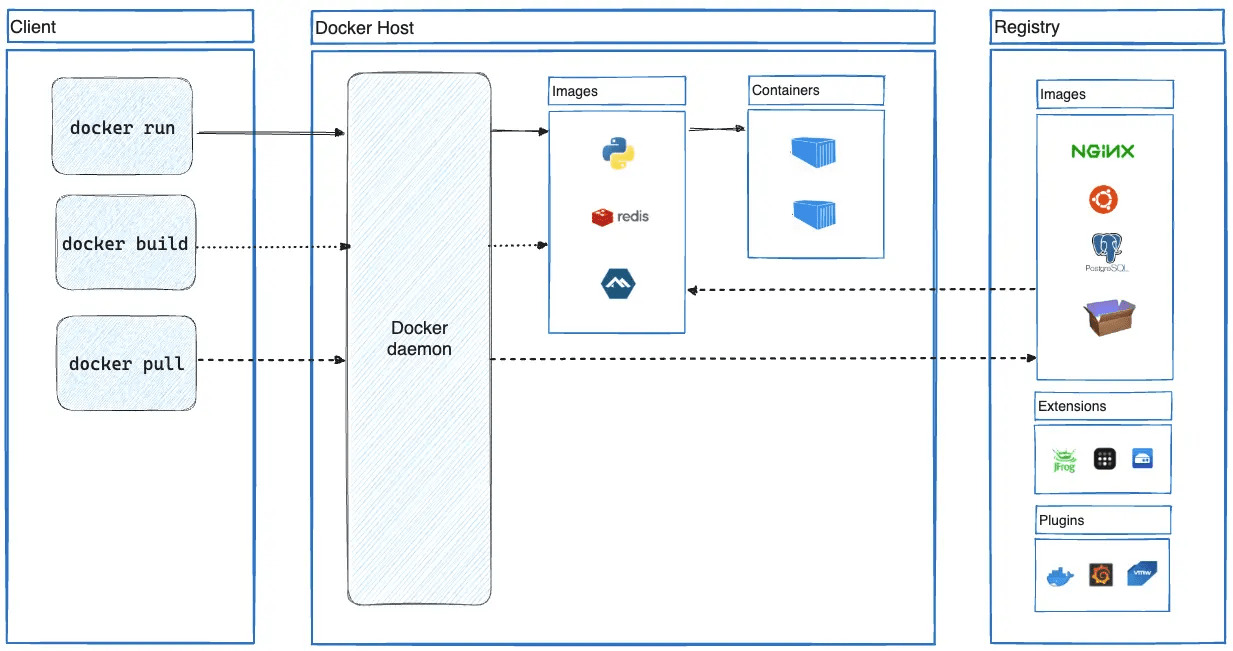
\includegraphics[width=12cm]{02_images/part_01/10_docker_architecture.png}
            \caption{Schéma de l'architecture Docker}
        \end{figure}

        L'adoption de Docker au sein de DASCH est donc stratégique. L'organisation a un Docker Hub dédié et cela permettra d'accélérer la livraison des applications et de les diffuser \footnote{Pour plus de détails sur les applications de \dsc sur Docker Hub, Voir \cite{daschswiss_dockerhub}.}.
        
    \clearemptydoublepage
    
    % \subsection{SEM NOME} SUBSTITUIR AO FIM DO PROCESSO NAO ESQUECER!
% SUBSTITUIR ANGLICISMES téléchargé ...
% INSÉRER L'IMAGE
\part{De l'image au standard IIIF : conceptions des \eng{pipelines}}
\chapter{Optimisation des images et objets pour IIIF : outils et méthodes}
    Le standard IIIF a ouvert de nouvelles voies pour la gestion et la visualisation de contenus numériques, notamment les images 2D et les modèles 3D. Cependant, l'intégration harmonieuse de ces différents types de ressources au sein de ce cadre reste un défi. Si des applications spécifiques ont été développées pour répondre à cette problématique \footnote{Par exemple, l'emploi de GIMP, Blender et MeshLab pour cette tâche est déjà connu dans le milieu patrimoniale, Voir \cite{raemygautschy2023}.}, leurs limites en termes de flexibilité et de maintenance ont rapidement été mises en évidence. C'est dans ce contexte que des chercheurs se sont tournés vers des solutions plus automatisées, telles que les scripts Python \footnote{Dans son article de 2023, Rossenova constate également ce problème, et cite l'exemple du \eng{The Smithsonian Cook} comme tentative pour contourner ce défi. Voir \cite{rossenova2023iiif}. Bien que l'étude de Ioannides et Patias ne se concentre pas spécifiquement sur cette question, il est intéressant de noter que, bien que récente, elle évoque les difficultés liées à la manipulation de modèles 3D sans aborder la possibilité d'utiliser des scripts Python. Cet ouvrage constitue néanmoins une réflexion précieuse sur les défis rencontrés dans ce domaine. Voir \cite{ioannides_patias_2023}.}.

    Dans cette étude, nous nous proposons d'explorer plus en détail les possibilités offertes par les \eng{pipelines} automatisés en Python pour traiter les défis liés à l'intégration de contenus 2D et 3D au sein du standard IIIF. En s'appuyant sur les travaux existants, nous présenterons ces \eng{pipelines}, capables de s'adapter à une grande variété de données.
    
    \section{Conception du \cvt}
    \cvt est une application conçue pour convertir des images aux formats .jpg, .jpeg et .png en versions plus légères. Il visait remplacer le logiciel GIMP.
        \subsection{Bibliothèques}
        Ce code Python utilise plusieurs bibliothèques pour effectuer la conversion et le téléchargement d'images redimensionnées. Voici un aperçu de chacune d'entre elles :
        
        \subsubsection{Flask}
        
        \begin{lstlisting}[language=Python]
        from ..app import app, ALLOWED_EXTENSIONS
        \end{lstlisting}
        
        Importe l'application \FSK \texttt{app} et la variable \textbf{ALLOWED\_EXTENSIONS} depuis un module parent nommé \texttt{app}. Cette variable contient une liste d'extensions de fichiers d'images autorisés pour le traitement qui sont les suivants : \textbf{.jpg}, \textbf{.jpeg} et \textbf{.png}.
        
        \subsubsection{io}
        
        \begin{lstlisting}
        from io import BytesIO
        \end{lstlisting}
        
        Importe la classe BytesIO du module io. Cette classe permet de créer un objet ressemblant à un fichier en mémoire, ce qui est utile pour conserver temporairement l'image redimensionnée avant son téléchargement.
        
        \subsubsection{flask}
        \begin{lstlisting}
        from flask import render_template, redirect, request, url_for, send_file:
        \end{lstlisting}
        
        Importe plusieurs fonctions utiles de Flask pour la gestion des requêtes \textsc{HTTP}. Par exemple, \textbf{render}\textunderscore\textbf{template} permet de rendre des templates HTML pour l'affichage des pages \eng{web} ; \textbf{redirect} redirige l'utilisateur vers une autre URL ; \textbf{request}: Donne accès aux informations de la requête en cours, y compris les fichiers téléchargés ; \textbf{url}\textunderscore\textbf{for}: Génère l'URL d'un endpoint Flask en fonction de son nom ; finalement, \textbf{send}\textunderscore\textbf{file}: Permet de renvoyer un fichier à l'utilisateur en téléchargement.

        \subsubsection{werkzeug.utils}

        \begin{lstlisting}
        from werkzeug.utils import secure_filename
        \end{lstlisting}
        
        Importe la fonction \textbf{secure}\textunderscore\textbf{filename} du module werkzeug.utils. Cette fonction sécurise le nom de fichier téléchargé afin d'éviter des problèmes potentiels de sécurité.

        \subsubsection{Pillow}
        
        \begin{lstlisting}
        from PIL import Image
        \end{lstlisting}
        
        Importe la classe Image du module PIL (aussi connu sous le nom de Pillow). Cette bibliothèque est utilisée pour la manipulation d'images en \py.
        
        \subsection{Fonctionnalités du code}
        Le code \py implémente une application \eng{web} simple qui permet aux utilisateurs de télécharger une image et de la redimensionner avant de la télécharger à nouveau. Voici une explication détaillée des différentes parties du code :
        
        \subsubsection{Configuration globale (en dehors des fonctions)}

        \begin{lstlisting}
        Image.MAX_IMAGE_PIXELS = None
        \end{lstlisting}
        
        Supprime toute limite imposée par Pillow sur la taille maximale des images en \eng{pixels}.
        
        \subsubsection{Fonction \textbf{allowed\_file} (filename)}
        
        Vérifie si l'extension du fichier téléchargé correspond à l'une des extensions autorisées conservées dans la variable \textbf{ALLOWED\_EXTENSIONS}.
        
        \subsubsection{Fonction \textbf{resize}\textunderscore\textbf{image}()}
        
        Ouvre l'image en utilisant le nom de fichier \textbf{filename} fourni. Calcule le rapport de réduction nécessaire pour que l'image ne dépasse pas les dimensions maximales définies par \textbf{max}\textunderscore\textbf{width} et \textbf{max}\textunderscore\textbf{height} (ici 1024x1024 \eng{pixels}).
        
        Redimensionne l'image en utilisant le filtre anti-aliasing \textsc{Lanczos} pour une meilleure qualité.
        Renvoie l'image redimensionnée.

        \subsubsection{Route @app.route("/")}

        Correspond à la racine de l'application.
        Renvoie le template \html principal conservé dans le dossier pages/main.html. Ce template est responsable de l'affichage du formulaire de téléchargement de l'image.

        \subsubsection{Route @app.route("/convert", methods=['POST'])}

        Correspond à l'URL /convert et ne gère que les requêtes \textsc{HTTP} de type POST (souvent utilisées pour les formulaires de téléchargement).
        Exécute la fonction \textbf{upload}\textunderscore\textbf{image} pour traiter le fichier téléchargé.
        
        \subsubsection{Fonction \texttt{upload\_image}()}
        
        Vérifie si le formulaire de téléchargement contient un fichier nommé "file". Si aucun fichier n'est présent, redirige l'utilisateur vers la même page.
        Récupère le fichier téléchargé depuis la requête et vérifie si son nom n'est pas vide. 
        Si le fichier est valide et son extension est autorisée (vérification par \texttt{allowed\_file}), sécurise le nom de fichier et récupère son extension.
        Redimensionne l'image en utilisant la fonction \texttt{resize\_image}.
        Crée un objet BytesIO pour conserver l'image redimensionnée en mémoire.
        Enregistre l'image redimensionnée dans l'objet.
        
    \section{Conception du \msh}
    \msh est une application conçue pour convertir des images 3D en versions plus légères à l'aide d'une méthode de simplification par décimation quadratique des arêtes, similaire à celle disponible dans des logiciels comme MeshLab.
    
        \subsection{Bibliothèques}
        
        Dans le cadre de cette étude, l'objectif était de développer une méthode permettant de réduire la taille des modèles 3D. Pour ce faire, le prérequis était de trouver une bibliothèque qui utilise la méthode de contraction \eng{Method Iterative Contraction Edges with Quadric Error Metrics}, telle qu'implémentée dans l'outil MeshLab. Cette technique, détaillée dans l'article de Garland et Heckbert, consiste à simplifier progressivement un maillage en contractant les arêtes les moins significatives \footnote{Cet algorithme est le développement d'un algorithme précédent, créé aussi pour les auteurs en 1997, dans lequel ils se sont intéressés seulement par la réduction de surfaces. Il est donc intéressant de souligner que cet article les auteurs ont envisagé bien les problèmes des modèles 3D : 
        ils souvent présentent d'autres propriétés, telles les couleurs, textures et surface normales, qui ont été finalement traitées en 1998. De plus, en effet l'usage de mémoire est réduite comme ils ont prévu. Pour l'article de 1997, Voir \cite{garland1997surface}. Pour l'article de 1998 sur le \eng{Method Iterative Contraction Edges with Quadric Error Metrics} qui sert de base à cette fonction utilisée sur MeshLab, PyMeshLab et Open3D, Voir \cite{garland1998quadric}.}.

        Afin de mettre en œuvre cette méthode, deux bibliothèques Python ont été étudiées : PyMeshLab et Open3D. Ces deux bibliothèques offrent des fonctionnalités de traitement de maillages 3D et font référence au méthode de contraction des arêtes pour les surfaces avec des couleurs et textures de 1998.

        Après une phase de tests comparatifs qui a eu lieu pendant trois semaines, la bibliothèque Open3D a été sélectionnée. En effet, PyMeshLab, bien que proposant un large éventail de fonctionnalités, s'est révélée peu performante sur des modèles de grande taille, entraînant des temps de calcul excessivement longs, et voire des boucles infinies.

        Open3D s'est avéré être une solution efficace pour réduire la complexité des modèles 3D. Les performances de cette bibliothèque seront analysées en détail dans la troisième partie de ce travail. Cependant, il convient de noter que Open3D ne permet pas de reproduire intégralement les paramètres de l'application MeshLab. Cette limitation restreint quelque peu la flexibilité de l'outil, bien que le cœur de l'algorithme de contraction des arêtes étant identique dans les deux bibliothèques, des résultats satisfaisants ont pu être obtenus. Finalement, voici une explication détaillée de chaque bibliothèque du code \textbf{main.py}:

        \subsubsection{Flask}

        \begin{lstlisting}
        from ..app import app, ALLOWED_EXTENSIONS
        \end{lstlisting}
        
        Importez l'application \FSK \texttt{app} et la variable \texttt{ALLOWED\_EXTENSIONS} depuis un module parent nommé \texttt{app}. Cette variable contient une liste d'extensions de fichiers d'images, de modèles 3D, de textures et de couleurs autorisés pour le traitement, qui sont les suivants : \textbf{.glb}, \textbf{.gltf}, \textbf{.jpg}, \textbf{.mtl}, \textbf{.obj}, \textbf{.ply}, \textbf{.png}, \textbf{.stl}, \textbf{.tiff}.

        \subsubsection{os}
        Non explicitement importée, mais utilisée dans la fonction \texttt{tempfile.\linebreak NamedTemporaryFile}. Fournit des fonctions pour interagir avec le système d'exploitation, telles que la création de fichiers temporaires.


        \subsubsection{io}
        
        \begin{lstlisting}
        import io
        \end{lstlisting}
        
        Importe le module io qui fournit des classes pour la manipulation de flux de données.

        \subsubsection{open3d}
        
        \begin{lstlisting}
        import open3d as o3d
        \end{lstlisting}
        
        Importe la bibliothèque open3d sous le alias o3d. Cette bibliothèque est essentielle pour le traitement de nuages de points et de maillages 3D. Elle permet de charger, manipuler, visualiser et exporter des données 3D. Dans cette étude, elle a été utilisée en combinaison avec la méthode de réduction de maillages \eng{Method Iterative Contraction Edges with Quadric Error Metrics}.

        \subsubsection{numpy}
        
        \begin{lstlisting}
        import numpy as np
        \end{lstlisting}
        
        Importe la bibliothèque \textsc{numpy} sous le alias np. \textbf{NumPy} est une bibliothèque fondamentale pour le calcul scientifique en \py. Elle fournit des structures de données multidimensionnelles (tableaux) et des fonctions efficaces pour les opérations matricielles et algébriques linéaires.

        \subsubsection{tempfile}
        
        \begin{lstlisting}
        import tempfile
        \end{lstlisting}
        
        Importe le module \texttt{tempfile} qui fournit des fonctions pour créer des fichiers temporaires.

        \subsubsection{flask}

        Importé à partir de \texttt{..app}, comme vu précédemment. Fournit des fonctionnalités pour la création d'applications \eng{web} en \py.

        \subsubsection{werkzeug.utils}

         Importé à partir de \texttt{..app}, comme vu précédemment. Fournit des utilitaires divers, dont la fonction \texttt{secure\_filename} utilisée pour sécuriser les noms de fichiers téléchargés.

        \subsection{Fonctionnalités du code}

        Ce code \py implémente une application \eng{web} qui permet aux utilisateurs de monter une image sur le site, la convertir en un maillage 3D simplifié et la renvoie en téléchargement.Voici une explication détaillée des différentes parties du code :

        \subsubsection{Fonction \texttt{allowed\_file}(filename)}
        Comme pour la fonction précédente, vérifie si l'extension du fichier mis en ligne correspond à l'une des extensions autorisées conservées dans la variable \texttt{ALLOWED\_EXTENSIONS}.

        \subsubsection{Fonction \texttt{simplify\_image}(filename)}

        \textbf{Création de fichier temporaire :}
        
        Utilise \texttt{tempfile.NamedTemporaryFile} pour créer un fichier temporaire avec l'extension \textbf{.obj}.
        Écrit le contenu du fichier téléchargé (représenté par \eng{filename}) dans le fichier temporaire. 
        Stocke le nom du fichier temporaire dans la variable \texttt{temp\_filename}.\\
        
        \textbf{Lecture du maillage :}
        
        Utilise la fonction \texttt{o3d.io.read\_triangle\_mesh} pour lire le fichier temporaire (considéré comme un maillage 3D au format \textbf{.obj}).
        Stocke le maillage lu dans la variable \texttt{mesh}.\\
        
        \textbf{Centrage du maillage :}
        
        Calcule la boîte englobante (bounding box) du maillage à l'aide de \texttt{mesh.get\linebreak\_axis\_aligned\_bounding\_box}.
        Récupère les coordonnées minimum et maximum de la boite englobante.
        Calcule le centre de la boite englobante.
        Calcule le vecteur de translation nécessaire pour déplacer le maillage vers son centre.
        Déplace le maillage en utilisant la fonction \textbf{mesh.translate}.\\
        
        \textbf{Simplification des maillages :}
        
        Utilise la fonction \textbf{mesh.simplify\_quadric\_decimation(number\linebreak\_of\_triangles}) pour simplifier le maillage. Le paramètre \texttt{target\_number\linebreak\_of\_triangles} est fixé à 65000 dans ce code. Cette fonction réduit le nombre de triangles du maillage en s'appuyant sur une méthode de décimation quadratique.\\
        
        \textbf{Calcul et rendu des normales :}
        
        Calcule les normales des sommets et des triangles du maillage simplifié à l'aide des fonctions \textbf{mesh\_simplified.compute\_vertex\_normals} et \textbf{mesh\_simplified.compute\_\linebreak triangle\_normals}. Les normales permettent d'obtenir un éclairage réaliste lors du rendu du maillage.\\
        
        \textbf{Sauvegarde du maillage simplifié :}
         
        Similaire à la création du fichier temporaire, il utilise \texttt{tempfile.\linebreak NamedTemporaryFile} pour créer un nouveau fichier temporaire avec l'extension \textbf{.obj}.
        Enregistre le maillage simplifié dans le fichier temporaire à l'aide de la fonction o3d.io.write

    
    \section{Structure de \cvt et \msh}
    Concernant la structure du code, les deux applications utilisent la même structure de dossiers avec de légères modifications adaptées à leur cas d'utilisation. Le modèle de dossiers de ces deux applications a été inspiré par celui proposé sur GitHub par Maxime Challon, l'un de mes professeurs à l'\enc \footnote{Voir \cite{challon_coursm2tnah_flask}.}. En ce qui concerne le code de \cvt, notre travail s'est bénéficié des idées de l'application PNG-to-JPEG \footnote{Voir \cite{herrera_2023_png_to_jpeg}.}.

    De plus, les deux applications sont publiées de manière privée sur mon propre GitHub et seront finalement rendues publiques une fois la soutenance de mémoire effectuée. Une autre étape consistera à mettre à disposition la version finale de ces applications sur le \eng{Docker Hub} de \dsc, qui, comme mentionné précédemment dans le Chapitre 4, sert à archiver et à mettre à disposition les applications développées par l'organisation.

    Concernant le \cvt, il est possible d'observer sa structure générale à partir de cette arborescence sur GitHub :

        % structure GitHub du \cvt
        \begin{figure}[h!]
            \centering
            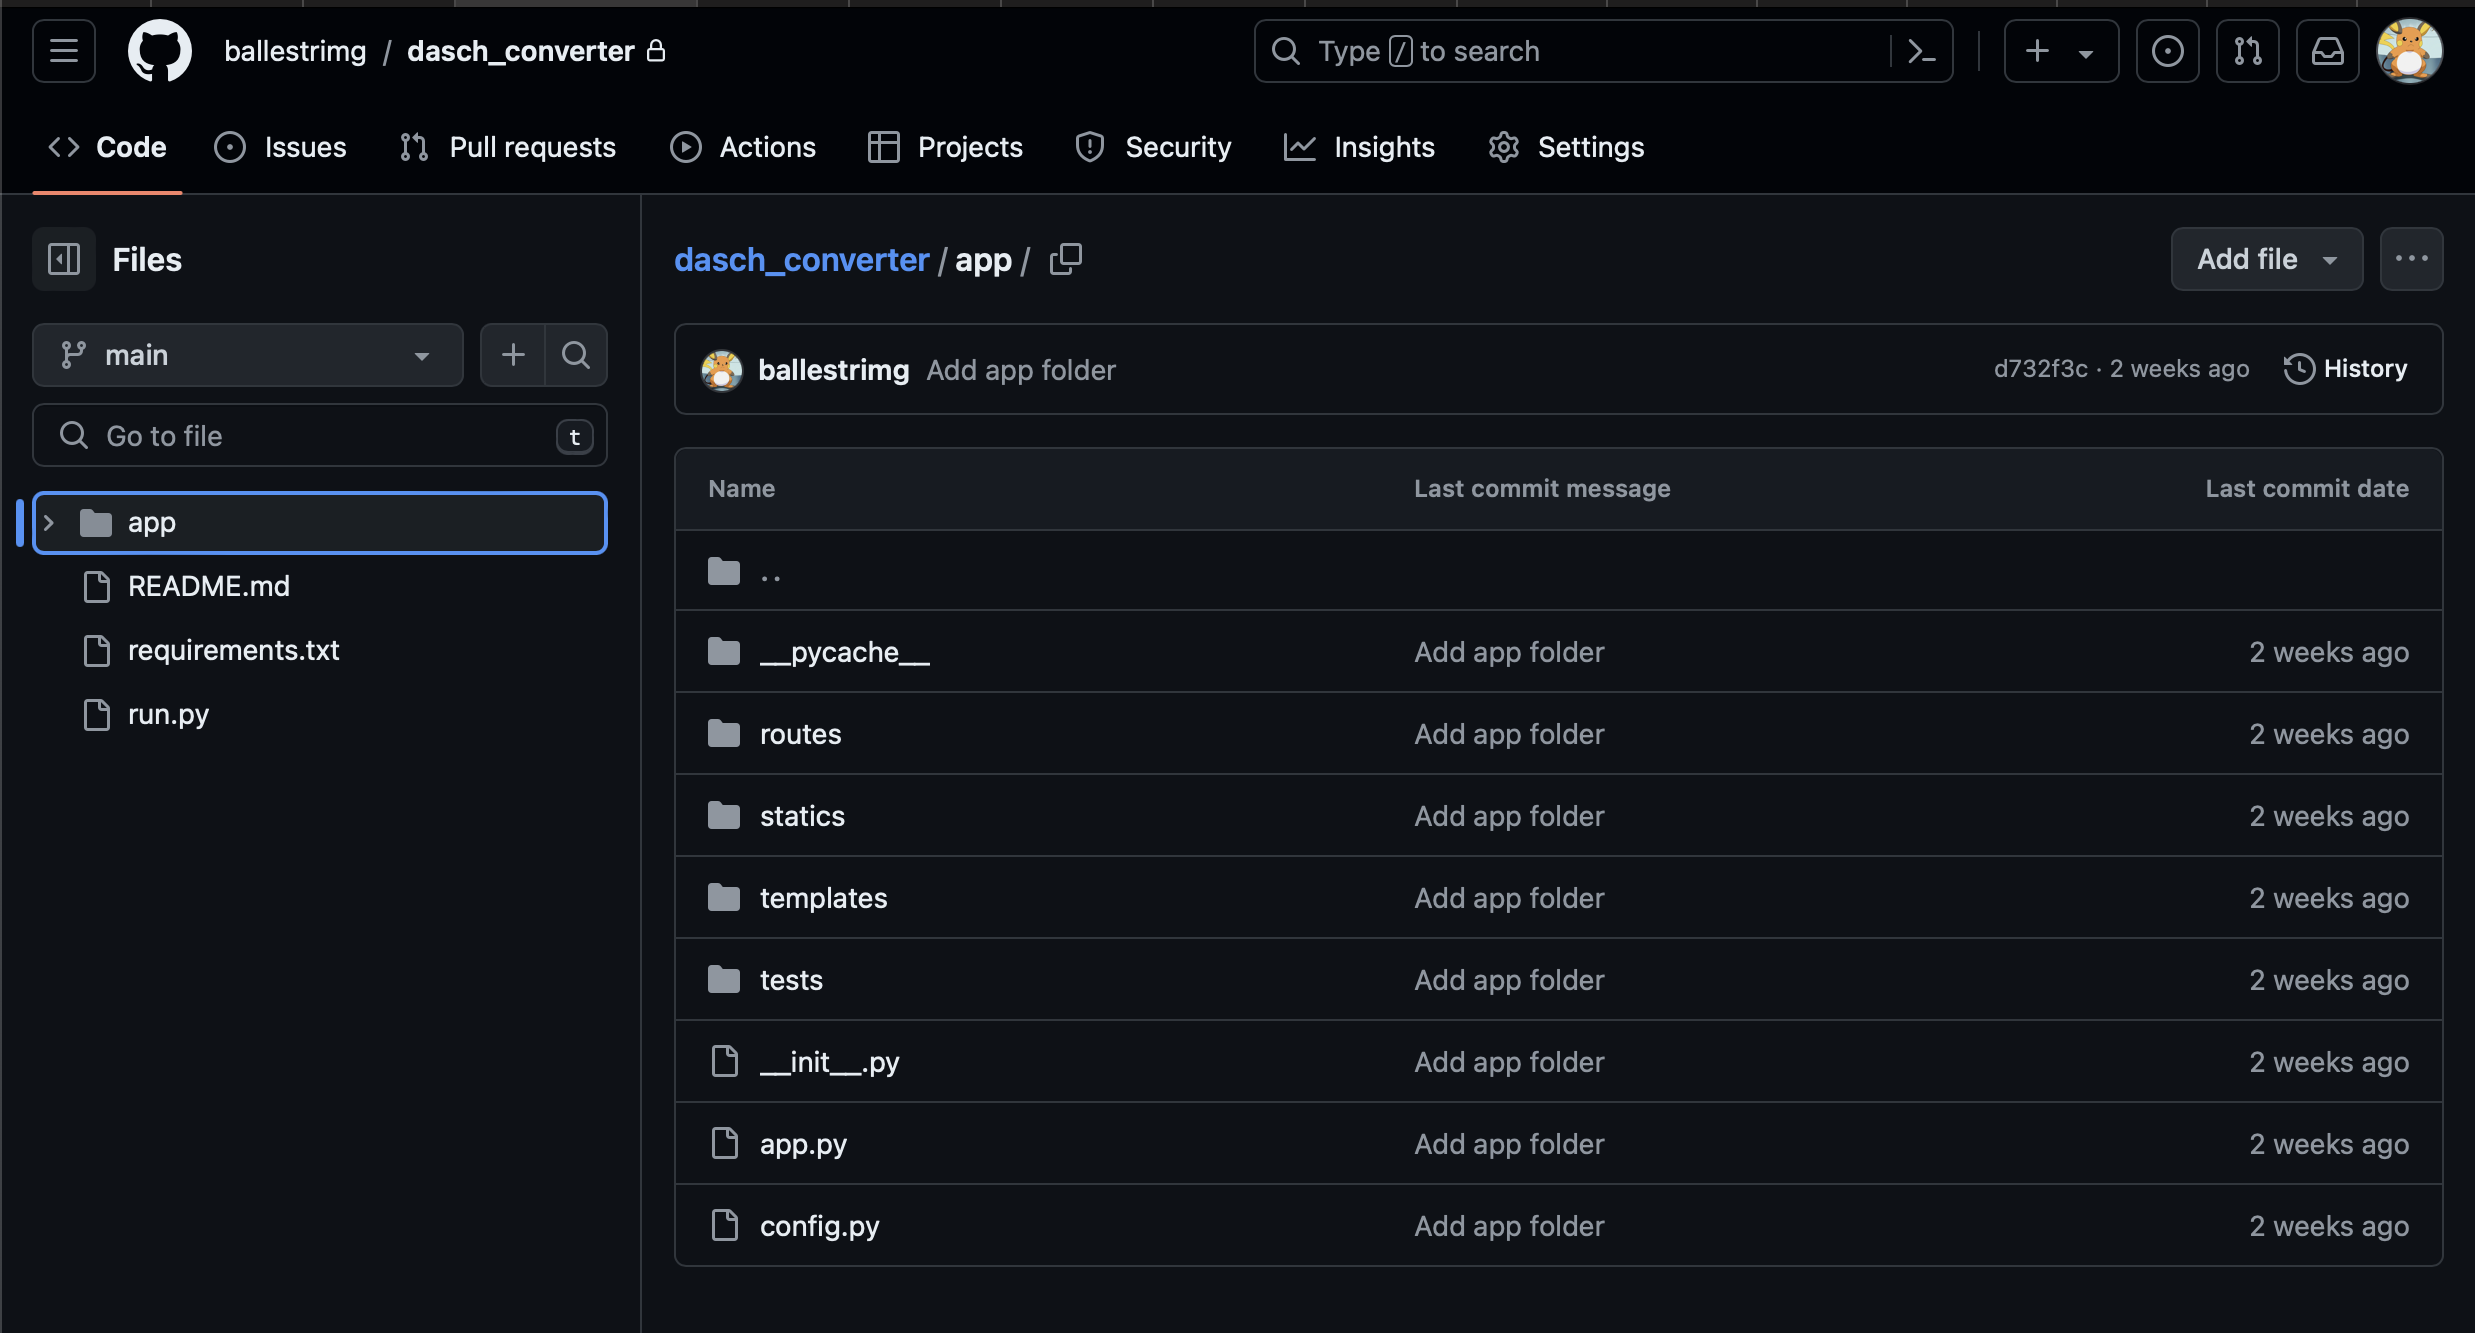
\includegraphics[width=12cm]{02_images/part_02/03_app_dasch_conv_github.png}
            \caption{Structure de l'application \cvt sur GitHub}
        \end{figure}

    Quant au \msh, sa structure est la suivante : 

    % structure GitHub du \msh
        \begin{figure}[h!]
            \centering
            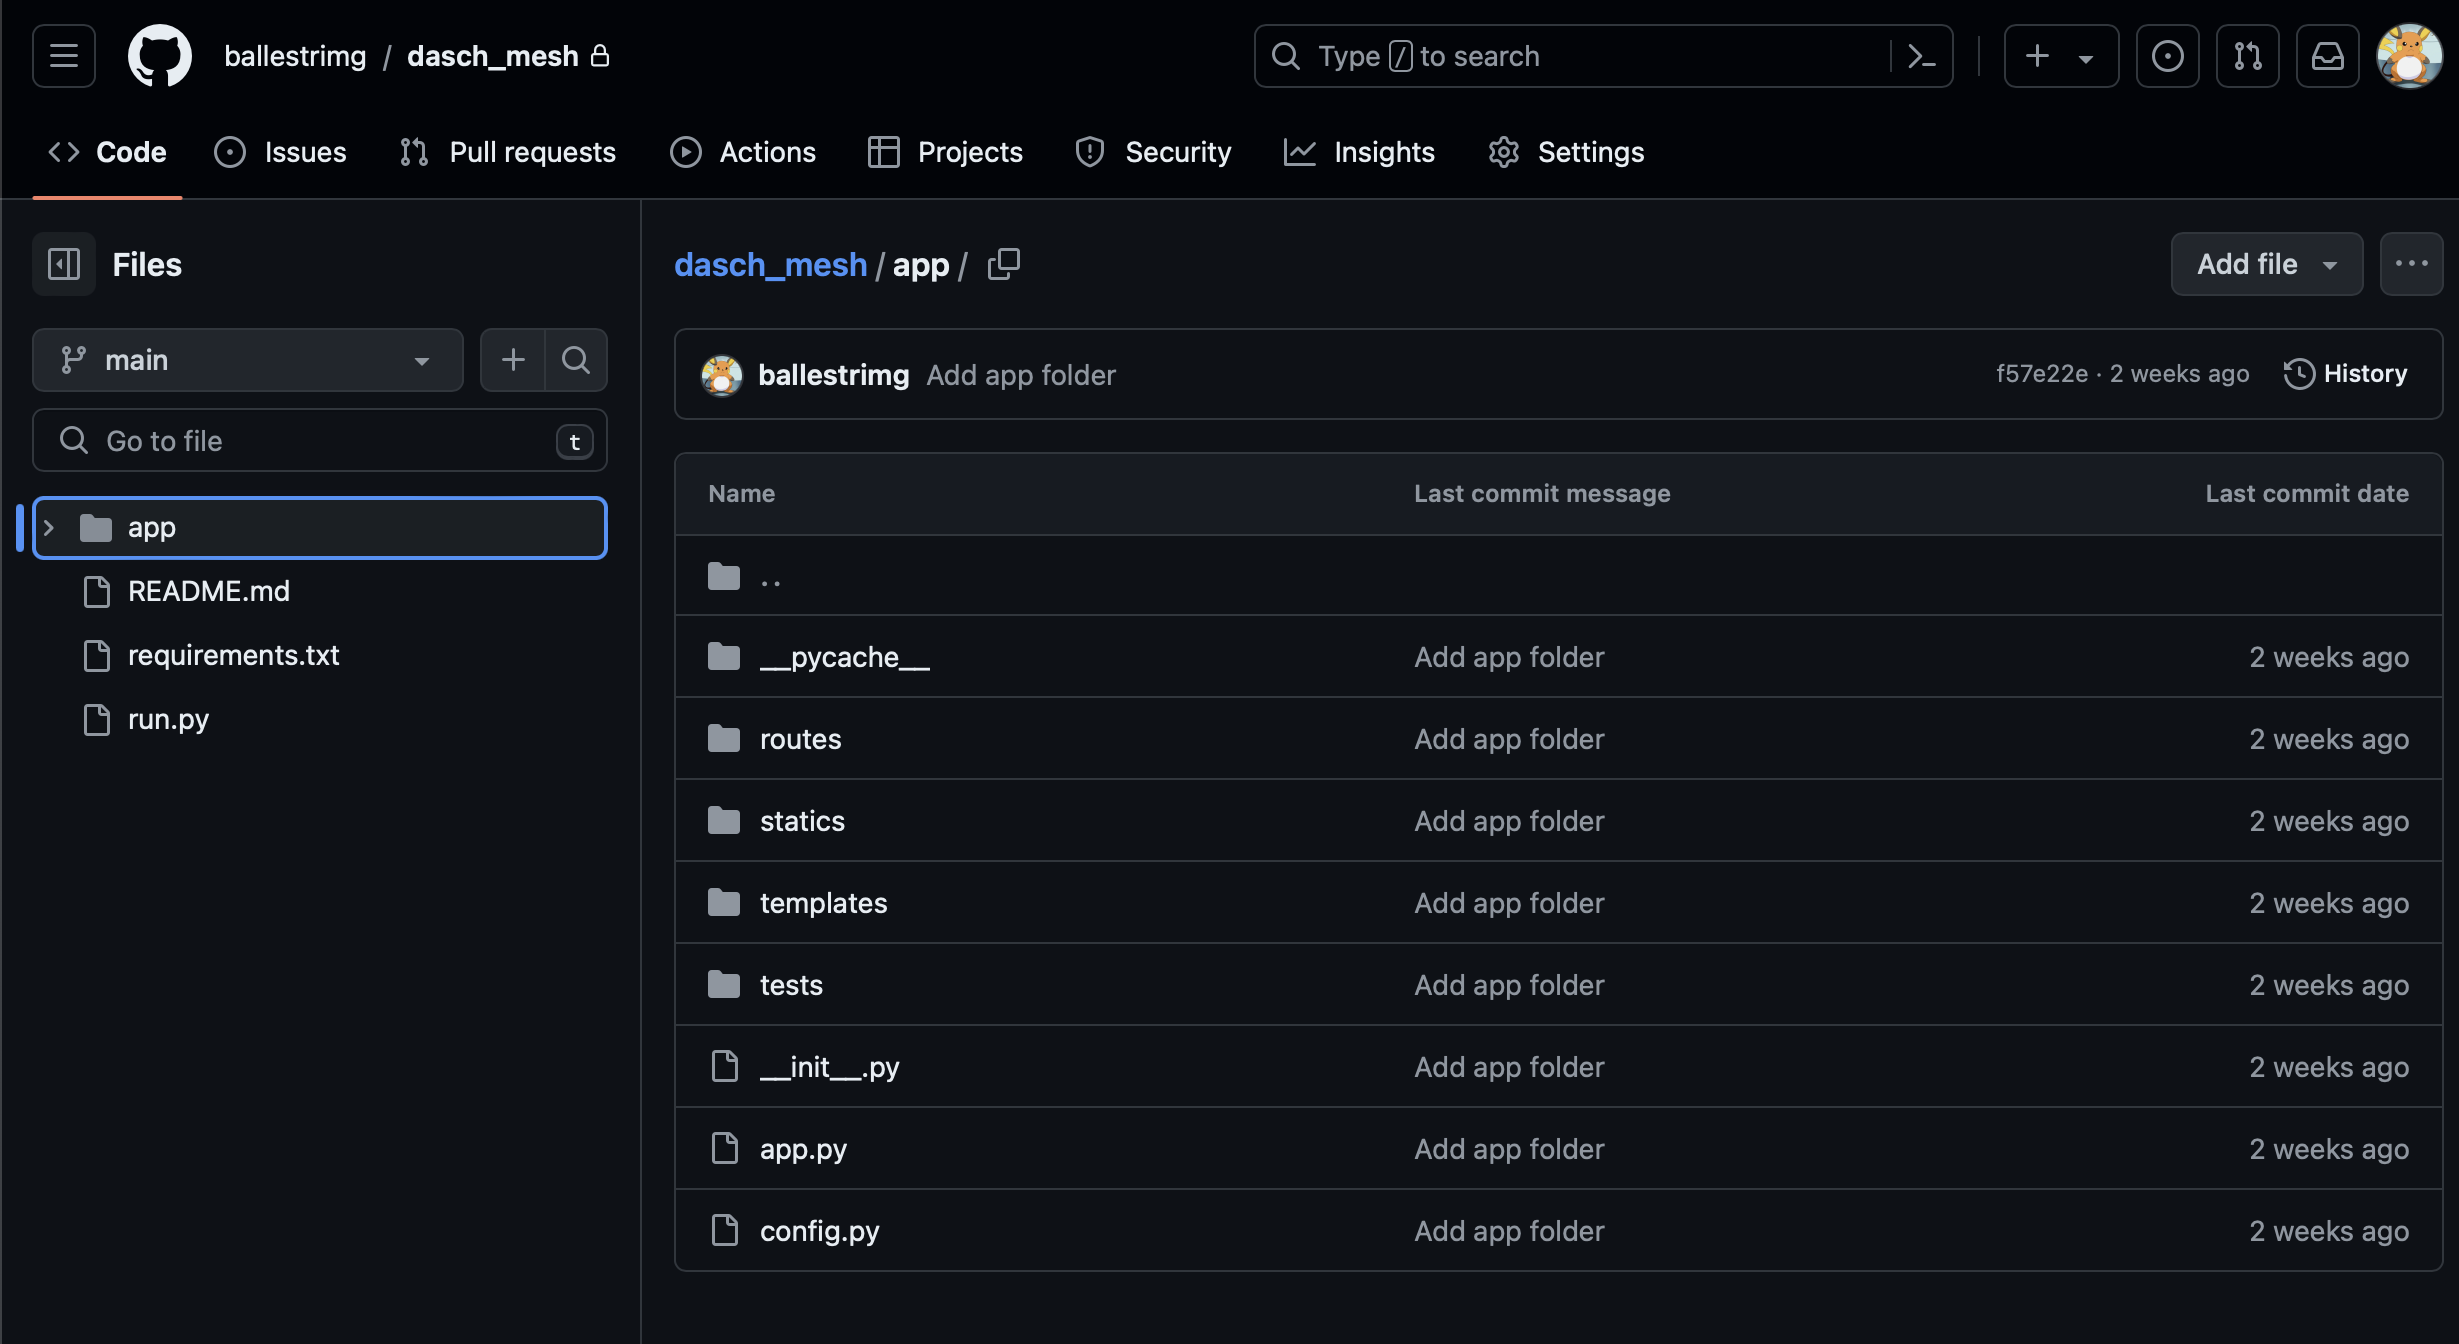
\includegraphics[width=12cm]{02_images/part_02/04_app_dasch_mesh_github.png}
            \caption{Structure de l'application \msh sur GitHub}
        \end{figure}

    L'arborescence des applications a pour but d'organiser les différents fichiers en dossiers, chacun correspondant à une fonctionnalité spécifique. Le dossier principal contient des sous-dossiers pour le code source, les tests, les données, la documentation et les fichiers de configuration. Cette structure permet une bonne séparation des préoccupations et facilite la maintenance du projet.
     
    Comme d'habitude pour les applications sur GitHub, on trouve un fichier \textbf{README.md} qui fournit une description du projet et un fichier \textbf{requirements.txt} qui liste les dépendances nécessaires pour exécuter l'application (bibliothèques, version Python, etc.). 

    Quant au \textit{design} de la page, il est inspiré du site \textbf{Smallpdf}. L'idée des boîtes pour y glisser des fichiers, ainsi qu'un bouton pour ajouter des contenus ont été utilisés en tant que principes des applications. 

        % structure GitHub du \msh
        \begin{figure}[h!]
            \centering
            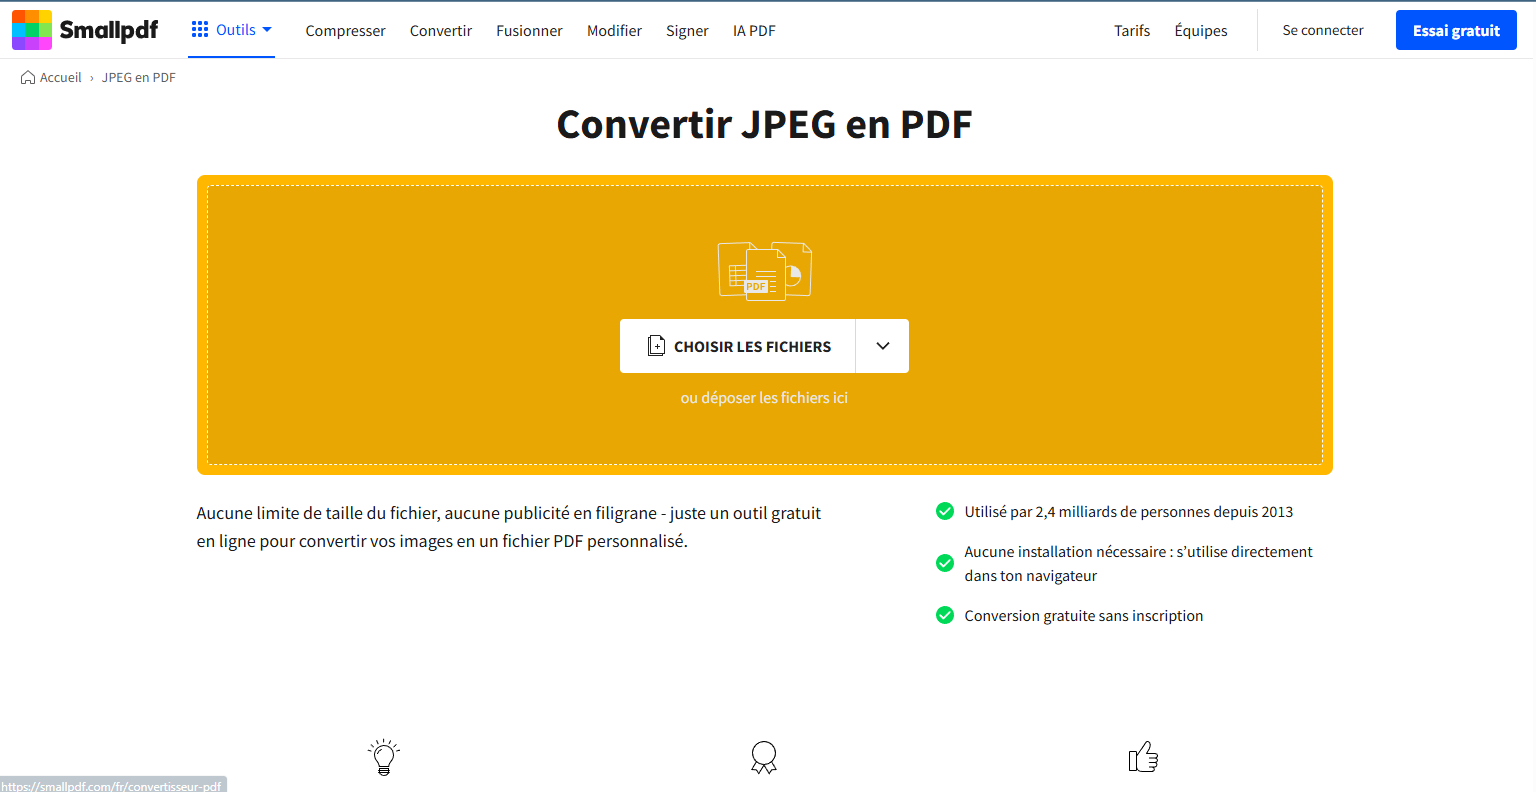
\includegraphics[width=12cm]{02_images/part_02/05_small_pdf.png}
            \caption{Page de convertion de fichier sur Smallpdf}
        \end{figure}
    
    Concernant les tests exécutés dans différentes versions \py, sur \eng{macOS M1} (\eng{Apple Silicon}) les versions \py pour \cvt et \msh ont été, respectivement, \textbf{3.11.0} et \textbf{3.9.0}~; sur \eng{Windows}, les deux applications ont utilisé la version \textbf{3.9.0} de \py~; les tests sur \eng{Ubuntu} \textbf{22.04.3} ont utilisé \py \textbf{3.10.12}. Il est important d'expliciter cela, car certaines bibliothèques comme \textsc{blinker 1.7.0} et \textsc{countourpy 1.2.1} n'acceptent pas des versions \py inférieures, respectivement, à \textbf{3.7.x} et \textbf{3.9.x}. De plus, jusqu'à ce jour, \textsc{open3d} fonctionne seulement dans les versions \py inférieures à \textbf{3.11.x}. A partir de Python 3.8, il est possible d'intégrer le framework Flask.

\chapter{Expérience utilisateur}
    \section{Intégration de l'UX dans les applications}
    
    Le développement de ces applications, \cvt et \msh, a mis en lumière l'importance de l'expérience utilisateur (\ux ou \eng{user experience}). Ce qui était autrefois perçu comme un domaine réservé aux designers s'est imposé comme un élément incontournable de la programmation, complétant la logique et le code de l'application. Dans ce chapitre, les raisons pour lesquelles l'intégration de l'\ux a été au cœur de nos préoccupations et comment il a été mis en œuvre seront discutés en détail.

    Pour mieux comprendre cette démarche, l'analyse abordera des différents aspects de l'application.

        \subsection{Vers une \ux inclusive}
        La conception d'applications numériques est souvent marquée par une dichotomie entre les utilisateurs experts, tels que les programmeurs et les administrateurs de plateformes, et les utilisateurs grand public, regroupant chercheurs, étudiants, amateurs et professionnels. Cette distinction, bien que pratique pour certains aspects de la conception, peut entraver la création d'une expérience utilisateur (\ux) véritablement inclusive. Or, en privilégiant un langage visuel efficace et en proposant une interface intuitive, notre application a cherché à combler ce fossé. En effet, en misant sur des éléments graphiques clairs et des interactions simples,  cet outil devient accessible à un large public, sans pour autant sacrifier les fonctionnalités attendues par les utilisateurs les plus expérimentés. Cette approche a permis de créer une expérience utilisateur unifiée, où les spécialistes peuvent tirer parti d'options avancées tout en offrant aux néophytes une prise en main rapide et efficace. Ainsi, en déconstruisant la traditionnelle opposition entre experts et grand public, notre application s'inscrit dans une démarche de démocratisation de l'accès aux outils numériques.

        \subsection{Fonctionnalités faciles à apprendre}
        Les deux applications ont été conçues pour répondre à un besoin spécifique : réduction de la taille des fichiers 2D et 3D. Pour atteindre cet objectif, les fonctionnalités simples et efficaces ont été mises en place, telles que le \eng{drag and drop} et les clics pour ajouter du contenu. Ces choix ont été guidés par le désir de minimiser la courbe d'apprentissage et de rendre l'application accessible à tous, y compris aux utilisateurs novices.

        \subsection{La palette de couleurs}
        La palette de couleurs a également été soigneusement sélectionnée. L'identité visuelle du \dsc a été maintenue tout en privilégiant des teintes qui ont la même couleur de l'association \footnote{De même pour la police de caractères \textsc{lato} \textsc{sans serif}, puisqu'elle est la police de \dsc.}. Les applications \cvt et \msh avaient, respectivement, les \eng{hex} couleurs \#336790 et \#74A2CF \footnote{Ces codes \eng{hex}, ainsi que les logos comme mentionné dans le Chapitre 2, ont été trouvés sur le document d'identité visuelle présent sur le compte Figma de \dsc. Il faut préciser que les codes de couleurs hexadécimaux, plus communément appelés codes \eng{Hex}, sont normalement composés d'un symbole dièse (\#) suivi de trois paires de chiffres représentant chacune les couleurs primaires RVB (rouge, vert, bleu). \cite{adobe_hex_codes}.}. Le choix de la couleur bleue avec peu de luminosité a deux raisons principales : en premier lieu, cette couleur est souvent associée dans notre culture à des entreprises reconnues telles qu'\eng{IBM} et \eng{Facebook} ; en deuxième lieu, sa basse luminosité et saturation suscitent plus d'émotions \footnote {Une étude menée avec des personnes de différentes cultures et niveaux de scolarité, fait pendant plusieurs années, a montré que la signification d'une couleur est plutôt influencé par sa luminosité et sa saturation et peu par sa teinte. C'est-à-dire qu'il n'y a pas une émotion liée de forme indissociable à une couleur à cause de sa teinte. Cela réfute l'idée reçue dans le design et la mode selon laquelle il y aurait une émotion universelle qui pourrait être associée à une couleur. En outre, pour les couleurs chaudes (\eng{warm-cool}) bien que la saturation et la teinte aient leur degré d'importance, les personnes n'avaient pas une opinion consistante sur quel aspect était le plus important, Voir \cite{crosscultemo}. Il est aussi intéressant de mentionner qu'une autre étude, plus ancienne, a déjà remarqué le fait que la perception visuelle est tellement complexe que d'autres aspects de nature distincte de la vision pourraient aussi jouer, tels que le goût, l'odeur et l'ambiance. Cela montre, encore une fois, l'importance de l'interdisciplinarité dans les champs d'études, Voir \cite{valberg2005}.}.

        % home page \cvt et \msh
        \begin{figure}[h!]
            \centering
            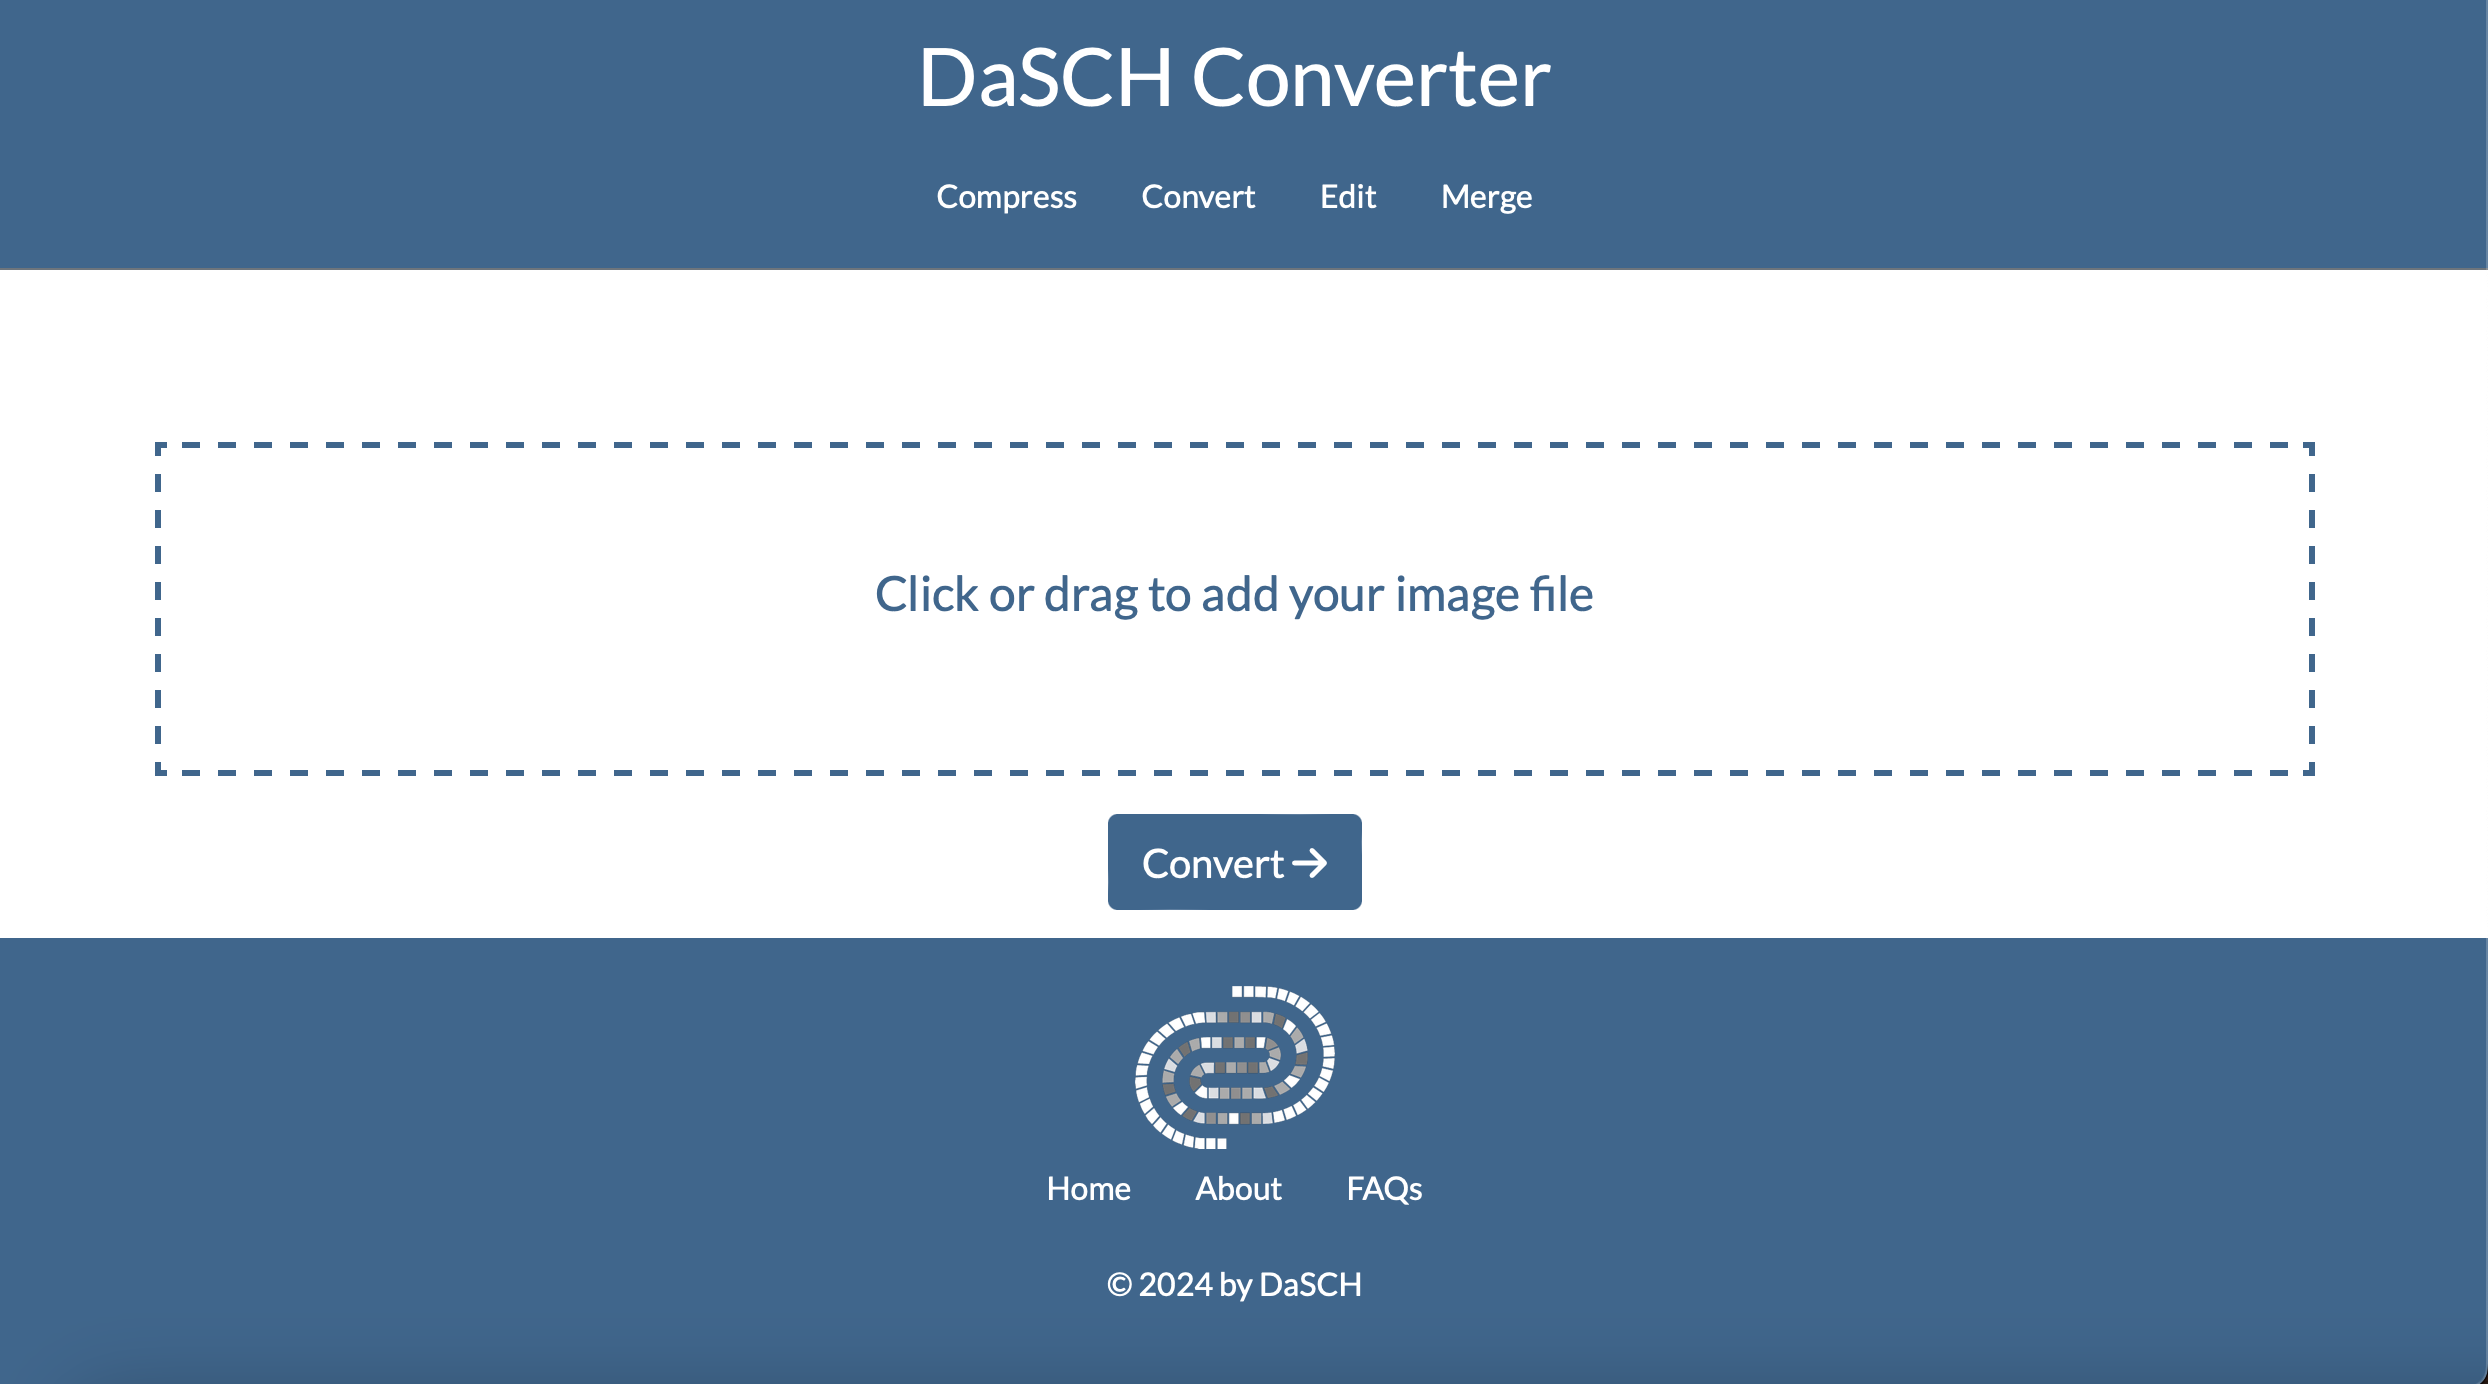
\includegraphics[width=8cm]{02_images/part_02/01_app_dasch_conv.png}
            \caption{Page principale du \cvt}
        \end{figure}

        % home page \msh
        \begin{figure}[h!]
            \centering
            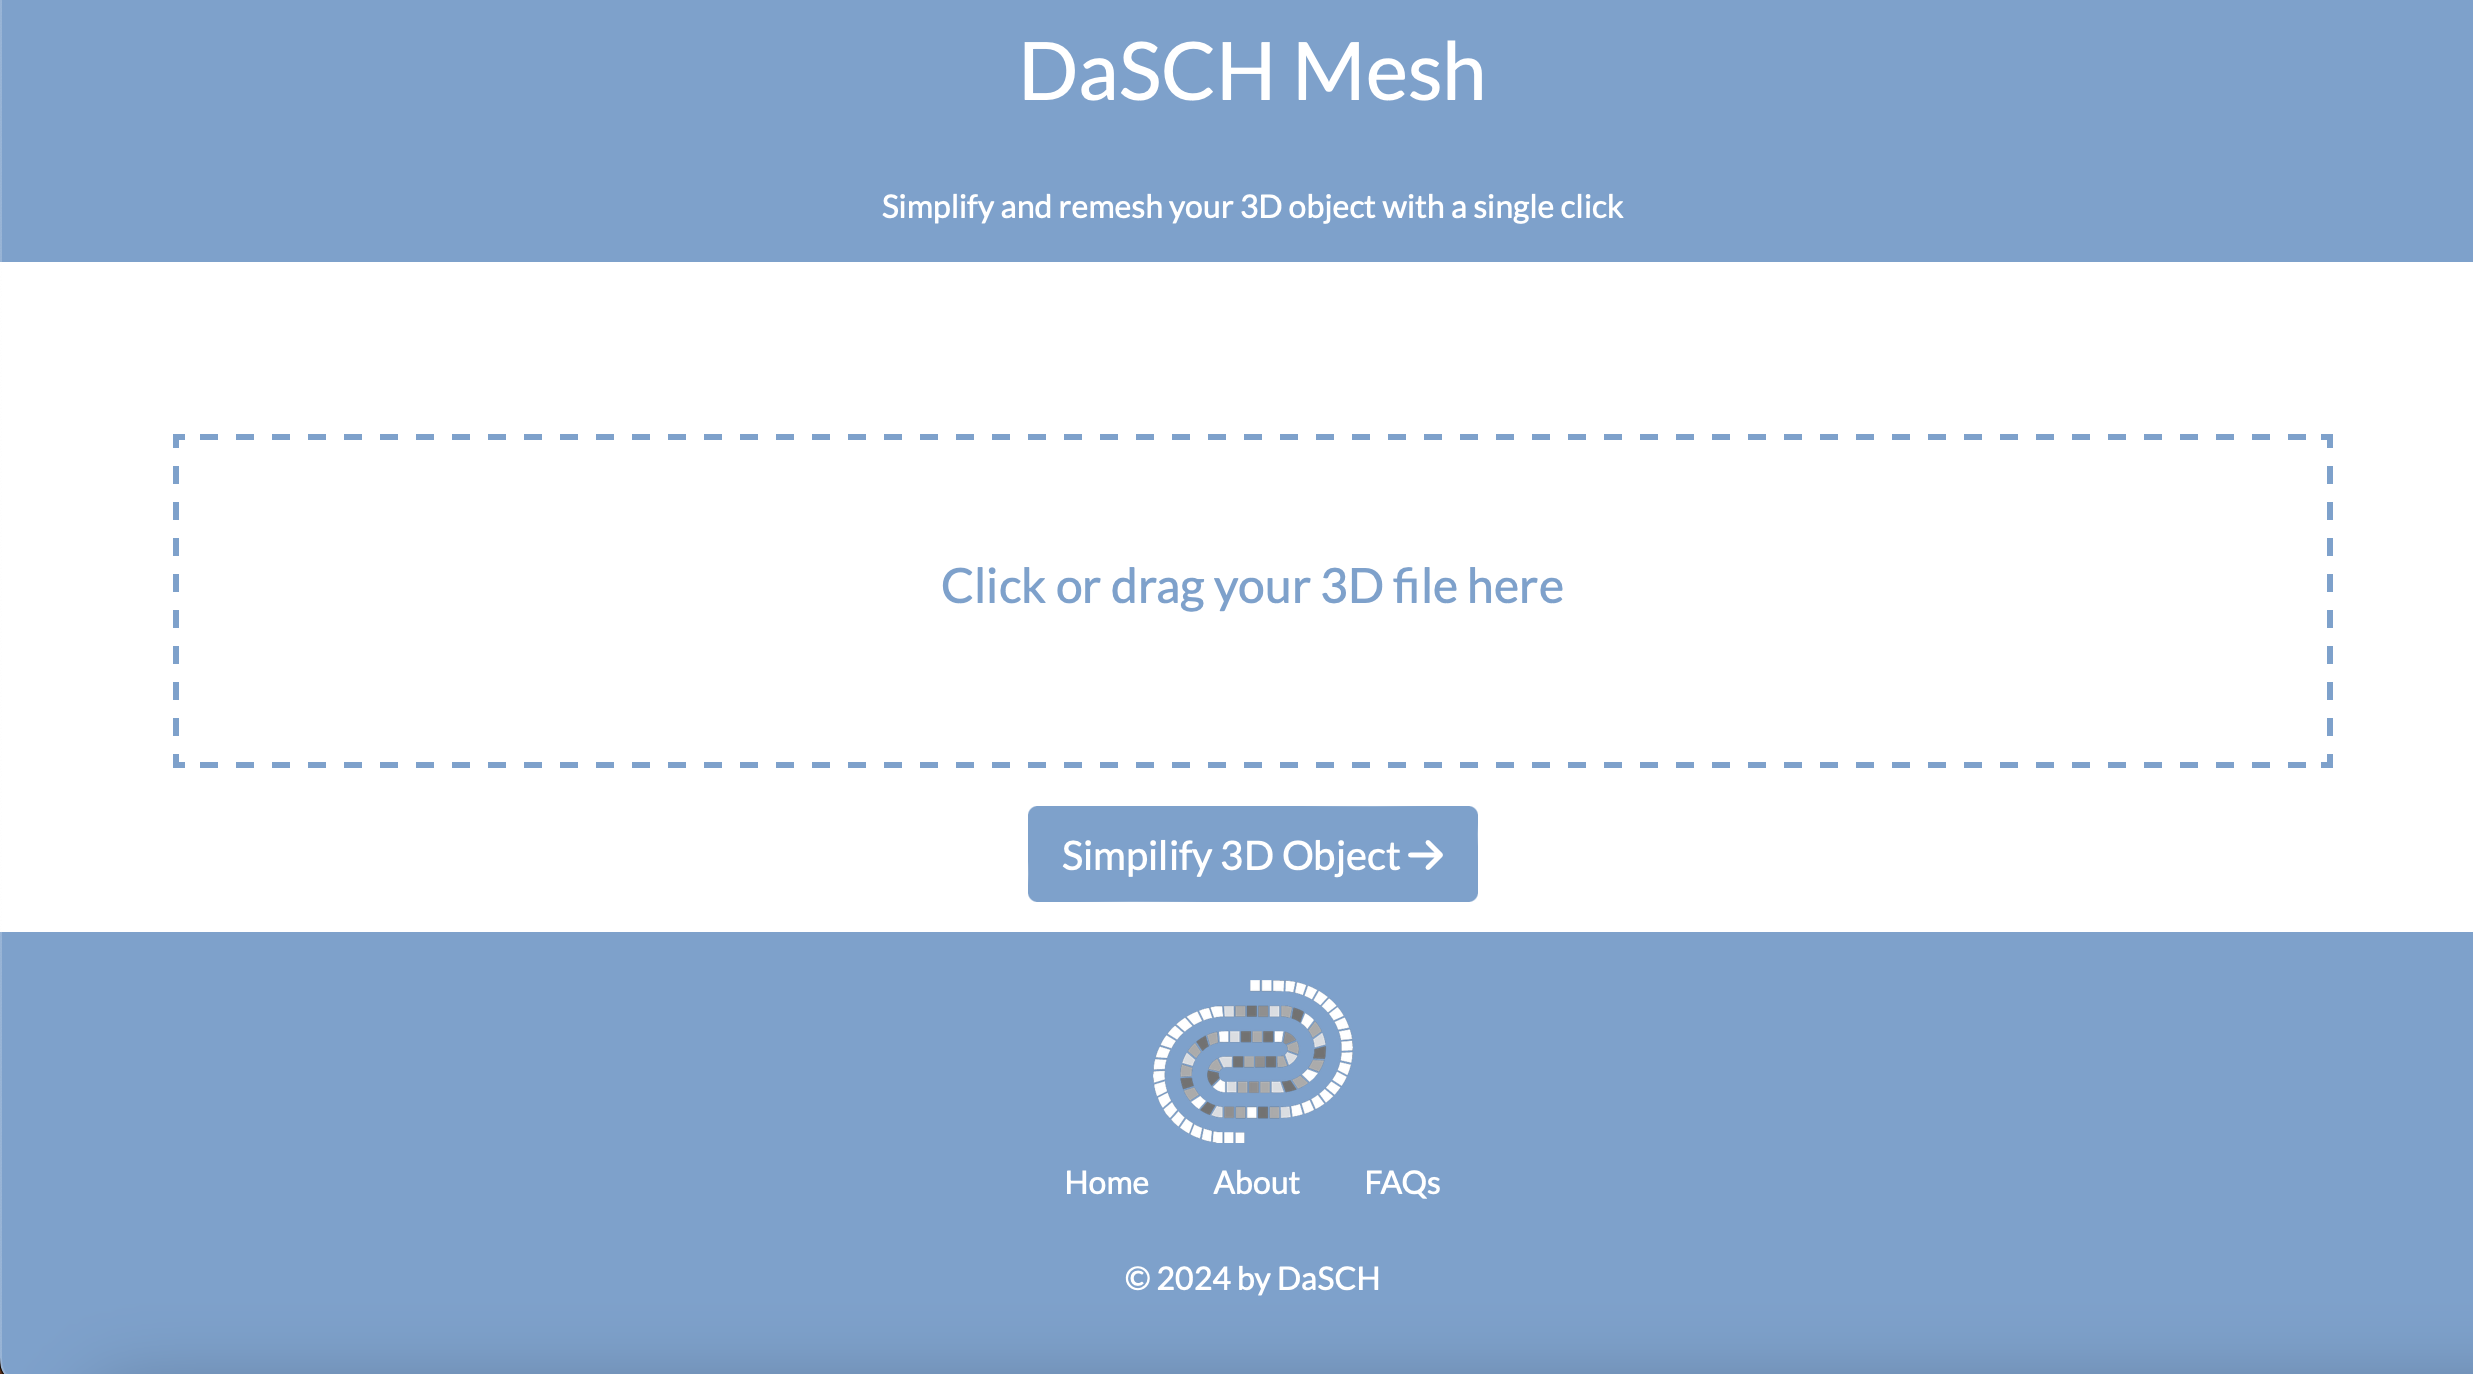
\includegraphics[width=8cm]{02_images/part_02/02_app_dasch_mesh.png}
            \caption{Page principale du \msh}
        \end{figure}
    
        \subsection{Fluidité de l'\ux}
        Enfin, une attention particulière à la fluidité de l'expérience utilisateur a été accordée. Le téléchargement automatique des fichiers une fois la conversion terminée permet de gagner du temps et d'éviter toute manipulation complexe. De plus, l'ensemble des fonctionnalités de l'application a été conçu pour être intuitif et auto-explicatif, ne nécessitant aucune connaissance préalable en informatique de la part de l'utilisateur.

        \subsection{UX et \gco}
        Un UX design minimaliste, caractérisé par une interface épurée et des fonctionnalités essentielles, s'inscrit naturellement dans une démarche éco-responsable. En effet, en réduisant l'encombrement visuel et en simplifiant les interactions, ce type de design contribue à diminuer la charge cognitive des utilisateurs, et aussi pour une prise de décision plus rapide des utilisateurs. Cela se traduit par une consommation moindre de ressources informatiques, telles que la mémoire et la puissance de calcul. De plus, un design minimaliste limite le nombre d'éléments à charger, ce qui optimise la vitesse de chargement des pages et réduit ainsi l'empreinte carbone liée à la consommation énergétique des serveurs.
        
        Enfin, l'intégration de l'\ux dans notre application s'est avérée être un choix stratégique essentiel. En privilégiant la simplicité de fonctionnalités, une courbe d'apprentissage courte et une esthétique soignée, ces applications répondent aux besoins du \dsc. Cet \ux minimaliste en allégeant les applications et en facilitant leur maintenance, permet des codes plus durables, plus accessibles et plus respectueux de l'environnement, tout en offrant une expérience utilisateur optimale. 
        
\chapter{Enrichissement métadonnée : vers les \textit{Scenes} IIIF}
    \section{Conception du \dsc IIIF}
    \diiif est un code \py encore en développement dont le but est enrichir des fichiers 3D avec des métadonnées conformes aux standard IIIF.
        \subsection{Modèles utilisés}
        L'\eng{IIIF Workbench} a été un modèle privilégie afin de regarder la structure base des dossiers contenant des images pour les \eng{Image API} et \eng{Presentation API} d'IIIF, ainsi que pour concevoir un fichier \textsc{json} \footnote{Nous avons utilisé ce site lors du cours \enquote{Anglais langue de l'informatique} dispensé par Edward Gray dans le cadre du master Technologies numériques appliquées à l'histoire à l'\enc. Voir référence \cite{gdmrworkbench}.}.
        
        Ce site nous permet d'envoyer des images qui sont archivées dans nos ordinateurs au site par le biais d'une compte GitHub, auxquels sont associés au \eng{Image API} 2.x ou 3.x. Par la suite, ces images vont avoir un fichier \textsc{json} associé, possédant un \textbf{id} qui permettra, entre autres choses, créer l'\eng{IIIF Manifest}. Dans ce sens, l'\textbf{id} est une information très importante lors de la conceptualisation, et c'est en même temps la caractéristique la plus basique qui autorise à un fichier \textsc{json} devenir un \eng{IIIF Manifest}. Muni de ces deux informations, la modélisation des données est plus profiteuse, une fois que cela montre une application qui enrichie des fichiers avec de métadonnées conformes aux standards d'IIIF.

        \subsection{Prérequis}
        Pour conceptualiser le fichier \textsc{json} avec les paramètres minimaux, le modèle utilisé était extrait de cet exemple d'IIIF \texttt{model\_origin.json} \footnote{Ce modèle minimal pour les modèles 3D, ainsi que d'autres avec plus de paramètres, peuvent être trouvés sur le GitHub d'IIIF. Cf \cite{iiif3dmodelorigin}.}:

        % model_origin.json
        \begin{figure}[h!]
            \centering
            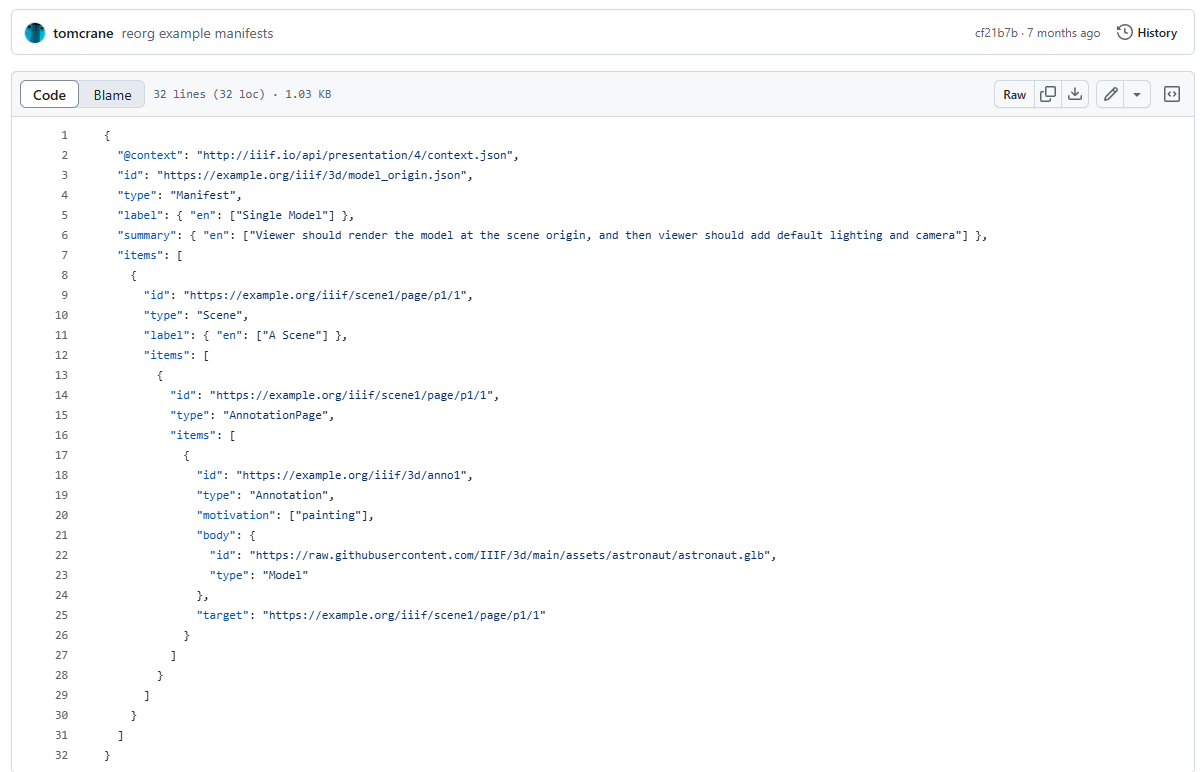
\includegraphics[width=12cm]{02_images/part_02/06_model.png}
            \caption{Code du fichier \texttt{model\_origin.json}}
        \end{figure}

        Il s'agit d'un fichier basique dans lequel force est de constater la présence d'un \texttt{id} qui permet d'utiliser cet objet et le conformer au standard IIIF.
        
        \subsection{Bibliothèques}
        Ce code \py utilise des bibliothèques, tels \textbf{os}, pour concevoir des fichiers \textsc{json}, qui sont les fichiers \eng{Manifest} IIIF, et pour travailler avec les fichiers d'entrée et de sortie.
    \clearemptydoublepage
    
    \part{Évaluation des outils et méthodes : bilan et perspectives}
\chapter{Performance des applications}
    \section{\cvt}   
    En examinant le graphique des tailles des fichiers PNG avant et après conversion avec GIMP et \py, il est clair que les fichiers PNG originaux sont généralement beaucoup plus volumineux que leurs versions converties en JPEG. Par exemple, le fichier \texttt{3DM\_FN170\_Mallet\_0.5mm\_filled\_ZG}, dont la taille originale est de 69,3 Mo, est compressé à 285,4 Ko avec GIMP et à 145,2 Ko avec \py. Cette réduction significative des tailles des fichiers PNG en JPEG est évidente pour tous les modèles étudiés. 
    
    Les différences entre les tailles obtenues avec GIMP et \py montrent que \py atteint des tailles de fichiers légèrement plus petites dans certains cas, ce qui pourrait refléter une compression plus efficace. Par exemple, pour le modèle \texttt{3DM\_TT95\_BL4\_1mm\_ZG}, \py réduit la taille à 294 Ko, contre 490,6 Ko avec GIMP. Cette tendance indique que l'application \py \cvt pourrait offrir une meilleure compression pour les fichiers JPEG, ce qui est important pour optimiser le stockage et la gestion des fichiers.

        \begin{table}[htbp]
            \centering
            \resizebox{\textwidth}{!}{
                \begin{tabular}{|l|l|l|l|}
                \hline
                \rowcolor{gray!20} % première ligne grise
                \textbf{Nom du fichier PNG} & \textbf{Taille originale} & \textbf{GIMP (JPEG)} & \textbf{Python (JPEG)} \\ \hline
                3DM\_FN170\_Mallet\_0.5mm\_filled\_ZG & 69,3 Mo  & 285,4 Ko  & 145,2 Ko \\ \hline
                3DM\_TT95\_BL4\_1mm\_ZG               & 38,9 Mo  & 490,6 Ko  & 294 Ko   \\ \hline
                3DM\_FN312\_FN313\_FN749\_FN789\_Sandstone\_0.5mm\_filled\_ZG & 116,9 Mo & 411,6 Ko & 217,8 Ko \\ \hline
                3DM\_FN571\_Sandstone\_0.5mm\_filled\_ZG & 42,9 Mo  & 244,8 Ko  & 134,1 Ko \\ \hline
                3DM\_TT95\_BL3\_1mm\_ZG               & 25,1 Mo  & 562,7 Ko  & 383,6 Ko \\ \hline
                \end{tabular}}
                \caption{Comparaison des tailles de fichiers avant et après conversion (GIMP et \cvt)}
        \end{table}

        % Graphe \cvt
        \begin{figure}[h!]
            \centering
            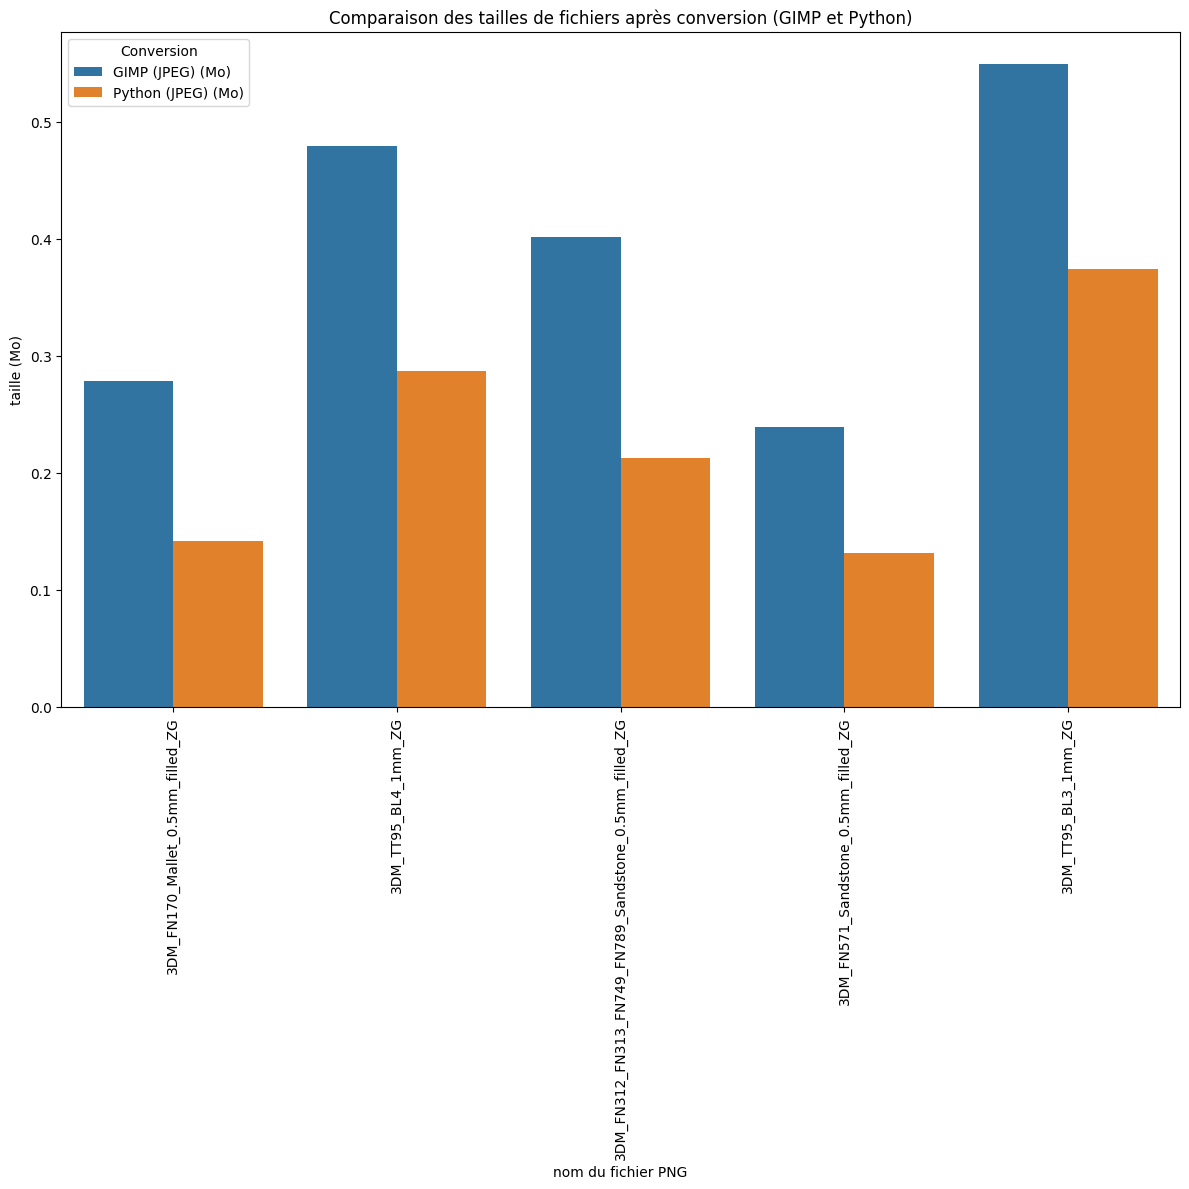
\includegraphics[width=13cm]{02_images/part_03/03_cvt_dv.png}
            \caption{Performance \cvt}
        \end{figure}
        
        
    \section{\msh}
 
    L'analyse des données sur les tailles des fichiers avant et après conversion révèle des informations cruciales sur l'efficacité des méthodes de compression utilisées. La réduction de la taille des fichiers est un facteur important dans le traitement et la gestion des données numériques, et les résultats obtenus permettent de comparer directement l'efficacité de différentes techniques de conversion.

    L'analyse du graphique illustrant les tailles des fichiers avant et après conversion avec MeshLab et \py met en évidence une réduction notable de la taille des fichiers grâce à l'utilisation de MeshLab. Par exemple, le fichier \texttt{3DM\_FN170\_Mallet\_0.5mm\_ZG}, initialement de 91 Mo, est réduit à seulement 6,78 Mo après conversion avec MeshLab, ce qui indique une compression significative. Cette tendance se confirme pour tous les modèles examinés, où MeshLab permet de réduire considérablement la taille des fichiers tout en limitant le nombre de sommets à 65 000. En comparaison, les conversions réalisées avec \py montrent une augmentation significative des tailles de fichiers dans la plupart des cas. Par exemple, le modèle \texttt{3DM\_TT95\_BL4\_1mm\_ZG} passe de 21,4 Mo avec MeshLab à 175,56 Mo avec Python, indiquant une augmentation notable de la taille des fichiers. 
    
        \begin{table}[htbp]
        \centering
        \resizebox{\textwidth}{!}{
            \begin{tabular}{|l|l|l|l|}
            \hline
            \rowcolor{gray!20} % première ligne grise 
            \textbf{Nom du modèle 3D} & \textbf{Taille originale} & \textbf{MeshLab (65k sommets)} & \textbf{Python (65k sommets)} \\ \hline
            3DM\_FN170\_Mallet\_0.5mm\_ZG & 91 Mo  & 6,78 Mo  & 21,56 Mo \\ \hline
            3DM\_TT95\_BL4\_1mm\_ZG      & 1,1 Go & 21,4 Mo  & 175,56 Mo \\ \hline
            3DM\_FN312\_FN313\_FN749\_FN789\_Sandstone\_0.5mm\_filled\_ZG & 625 Mo & 7,06 Mo  & 107,46 Mo \\ \hline
            3DM\_FN169\_Mallet\_ZG       & 157 Mo & 14,4 Mo  & 14,7 Mo \\ \hline
            3DM\_FN1848\_Mortar-3Cone\_Imprints & 22,8 Mo & 12,8 Mo & 4,6 Mo \\ \hline
            \end{tabular}}
        \caption{Comparaison des tailles de fichiers avant et après conversion avec MeshLab et \msh}
        \end{table}

        % Graphe \mshs
        \begin{figure}[h!]
            \centering
            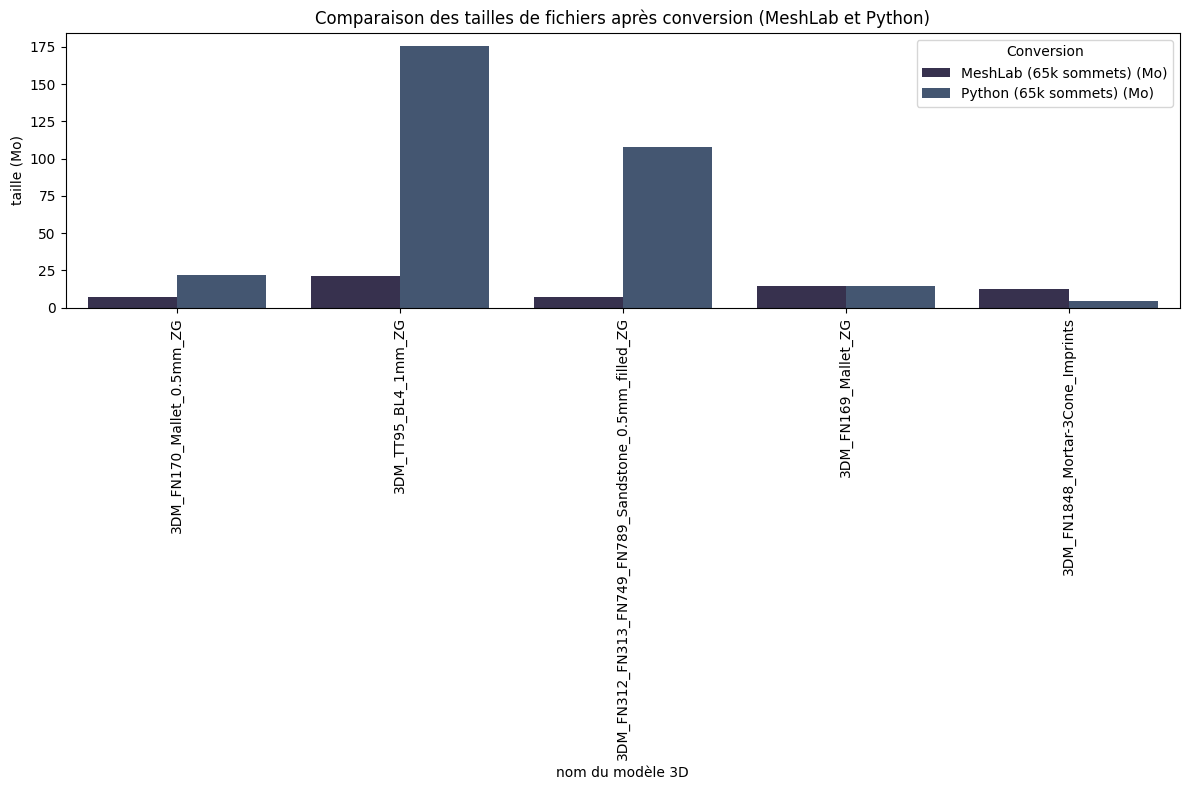
\includegraphics[width=13cm]{02_images/part_03/04_msh_dv.png}
            \caption{Performance \msh}
        \end{figure}

        Cela suggère que l'application \py \msh n'a pas encore été aussi efficace dans la gestion de la compression des fichiers pour les données 3D que MeshLab. Une explication plausible pour la baisse significative des performances pourrait résider dans l'utilisation de la bibliothèque Open3D. En effet, cette dernière n'offre pas les mêmes options de configuration que MeshLab. De plus, bien que la bibliothèque PyMeshLab offrait les mêmes options de configuration que MeshLab \footnote{Voir \cite{pymeshlab_decimation}.}, elle engendrait des boucles infinies lors de la conversion de fichiers volumineux. Pour de futures implémentations, il pourrait être envisagé d'utiliser Open3D ou d'explorer d'autres solutions au sein de PyMeshLab.
        
        
\chapter{Perspectives d'évolution : fonctionnalités supplémentaires}
    \section{Implémentations plus imminentes}

    Le développement logiciel est un processus collaboratif. Un programme est rarement le fruit du travail d'un seul développeur, mais plutôt le résultat d'une chaîne de contributions successives. Les codes sources sont partagés, modifiés, améliorés par différents acteurs au fil du temps. Cette nature collaborative du développement nécessite également une gestion rigoureuse des versions et une documentation précise pour garantir la cohérence du projet. Pour cette étude, les applications ont encore des implémentations à faire et voire des améliorations conséquentes.
    
    En ce qui concerne la gestion d'erreur, les deux applications \cvt et \msh en présentent une gestion sommaire. Seules les erreurs 404 et 500 ont été traitées, respectivement avec un modèle de \eng{template} qui affiche des images lors de l'erreur. Il serait intéressant de travailler ces erreurs pour les prochaines étapes du développement.

    Il serait pertinent d'intégrer des écrans de chargement lors du traitement de fichiers volumineux. L'objectif est de maintenir l'utilisateur au sein de l'application pendant toute la durée de l'opération. Une simple barre de progression, dont de noMoreux modèles sont disponibles sur Bootstrap par exemple, pourrait suffire \footnote{ces icônes de chargement d'un composant ou d'une page sont appelés de \eng{spinners}. Pour les exemples, Voir \cite{bootstrapspinners}.}.
    
    \section{D'autres implémentations possibles}
    \cvt et \msh, comme dit, ont été codés en \py à cause des raisons spécifiés dans la chapitre 4, à savoir : . néanmoins, ces applications peuvent, une fois finies et distribuées sur le \eng{DockerHub} de \dsc, être codées avec d'autres langages dont l'accent est mis sur la gestion de données et la performance, à l'instar de \textsc{rust} et \textsc{go}. 

    Les temps de réponse, en particulier pour les fonctionnalités qui nécessitent le traitement de grandes quantités de données, serait aussi une possibilité d'amélioration. Cela pourrait inclure la refactorisation du code pour le rendre plus efficace, l'implémentation de techniques de mise en cache, qui n'ont pas pu être développés lors du stage. 
    
    Par ailleurs, le recours à l'apprentissage automatique offre de nouvelles perspectives pour optimiser le processus de \msh. En entraînant un modèle sur un ensemble de données variées, il devient possible d'automatiser la classification des images et des objets, et ainsi de proposer des traitements adaptés à chaque type de fichier. Par exemple, en fonction de la présence ou de l'absence de textures, le modèle pourrait sélectionner automatiquement les algorithmes de conversion les plus pertinents (par exemple, un méthode A pour les fichiers sans texture et un méthode B pour les fichiers texturés). Cette approche permettrait de personnaliser davantage le processus de conversion et d'améliorer la qualité des résultats.

    L'interface utilisateur de l'application pourrait également être enrichie afin de faciliter l'utilisation et d'améliorer l'expérience utilisateur. En effet, il serait pertinent de développer des fonctionnalités permettant d'identifier rapidement les fichiers téléchargés.

    Pour répondre aux besoins des utilisateurs ayant de grands volumes de fichiers à convertir, il serait intéressant d'implémenter une fonctionnalité permettant de traiter plusieurs fichiers simultanément. Cette option permettrait de gagner en productivité et de simplifier le flux de travail. En outre, la création d'une liste de téléchargement pourrait être proposée afin de permettre à l'utilisateur de suivre l'avancement des conversions et de télécharger les fichiers résultants de manière organisée.
    
    En ce qui concerne \diiif, même si l'application n'est pas finalisée, il est concevable de tirer quelques pistes : dans un premier temps, l'inspiration serait créer une application intuitive, similaire à \cvt et \msh, car en termes d'\ux, elles sont intéressantes pour avoir intégré des éléments importants du \gco ; deuxièmement, transformer le code en application et le diffuser sur \textsc{docker} serait aussi un moyen de le rendre accessible au plus grand noMore d'utilisateurs possible.

\chapter{Outils de travail}
    \section{Aspects techniques}
    Tout d'abord, l'étude a bénéficié d'un MacBook Air équipé d'un processeur M1 d'Apple Silicon, offrant ainsi un outil performant et portable pour mener à bien les différentes tâches de la recherche.
    
    De plus, un disque dur externe contenant l'ensemble des données du projet DaSCH a été mis à disposition, permettant ainsi la mise en œuvre de \eng{pipelines} d'analyse automatisés. La portabilité de ce support a favorisé une grande flexibilité dans le déroulement des travaux.

    En somme, l'ordinateur ainsi que la disponibilité des données ont permis de mener des analyses approfondies, notamment des tests de performance, favorisant ainsi une exploitation optimale des données. Le télétravail a également été facilité grâce à cette configuration. À l'issue du stage, le MacBook Air a été restitué. En revanche, le disque dur externe nous a été attribué.

    \section{Gestion du temps}    
    Le déroulement du stage s’est distingué par une grande autonomie et une organisation méthodique, structurée en petites tâches hebdomadaires, gérées à l’aide de l’outil \textsc{trello}. Ce tableau de tâches, partagé avec \rg, la superviseure du stage, a permis un suivi rigoureux de l’avancement des \eng{pipelines} tout en servant de base pour les réunions hebdomadaires. Ces réunions, associées à cette approche structurée, ont favorisé une productivité réaliste, offrant un équilibre entre suivi et liberté. Elles ont également permis l’établissement d’un dialogue constructif, où des solutions, réflexions, et pistes d’amélioration ont pu être explorées pour débloquer certains problèmes, tout en offrant une compréhension approfondie du métier de la superviseure.

        % structure GitHub du \cvt
        \begin{figure}[h!]
            \centering
            
\includegraphics[width=10cm]{02_images/part_03/01_trello_logo.png}
            \caption{Logo de l'application \textsc{trello}}
        \end{figure}
    
    Au sein du projet DaSCH, la communication se faisait principalement par le biais d'une suite d'outils \eng{Google Workspace}, mettant à disposition des chercheurs une boîte mail professionnelle et un espace de travail collaboratif. Les échanges instantanés, particulièrement fréquents, étaient privilégiés via la messagerie instantanée de \eng{Google Chat}. Par ailleurs, l'outil \eng{Google Meet} était largement utilisé pour les réunions en ligne, offrant ainsi la possibilité de conférences et de partages d'écran en temps réel.

    En ce qui concerne les réunions, deux formats principaux étaient privilégiés. Des réunions d'équipe hebdomadaires permettaient de faire le point sur l'avancement du projet et de coordonner les tâches. Afin d'assurer un suivi régulier de l'exécution des codes, comme mentionné, il y avait aussi des réunions hebdomadaires dédiées. Ces rendez-vous réguliers ont permis de garantir une progression efficace du développement et de lever rapidement les éventuelles difficultés rencontrées. Cela n'a pas empêché de réaliser d'autres réunions entre les meMores de l'équipe, mais celles-là étaient moins régulières. 
    
    En ce qui concerne le travail de codage, un accord a été établi dès le début du stage pour que les horaires du stage soient organisées selon la technique Pomodoro, qui est une technique créée en 1992 pour réaliser une gestion efficace du temps \footnote{D'après Cirillo, cette technique, répandu dans le milieu du mangament depuis le final des années 90, a pour but, entre autres, améliorer le processus de travail et d'études. Voir \cite[p.~20]{cirillo2009}.}. Pour ce faire, l’application utilisée pour compter les minutes, nommée \textsc{flow}, a permis de structurer le temps en quatre sessions de 25 minutes avec des pauses de 5 minutes, suivies d’une longue pause de 30 minutes après le quatrième cycle. Cette méthode visait à améliorer la concentration lors de l’exécution des tâches, rendant le travail plus efficace. Dans le cadre de ce stage, la technique a contribué au développement de deux applications tout en aidant à trouver un rythme de travail adéquat.

        % structure GitHub du \cvt
        \begin{figure}[h!]
            \centering
            
\includegraphics[width=10cm]{02_images/part_03/02_flow_macos_logo.png}
            \caption{Logo de l'application \textsc{flow}, disponible que pour les \eng{macOS} et \eng{iOS}}
        \end{figure}

    La participation aux réunions, bien que non obligatoire pour les stagiaires, s'est révélée extrêmement bénéfique. Ces réunions ont offert une compréhension globale du travail, ainsi qu'une vision claire du fonctionnement quotidien d'un groupe de travail en sciences humaines. Cette immersion a permis la conception d'applications réalistes, tenant compte des spécificités de chaque groupe, et l'identification d'axes d'amélioration. De plus, cette expérience a enrichi la maîtrise de l'anglais et a fourni l'opportunité d'apprendre à gérer un projet de codage en collaboration avec plusieurs acteurs, facilitant ainsi une meilleure compréhension de la contribution de chaque partie à la réussite du projet.

    En conclusion, ce stage a été une expérience enrichissante à plusieurs niveaux. L’autonomie dans l’organisation du travail, la méthode structurée de gestion du temps, et l’implication active dans les réunions ont non seulement permis la réalisation d’applications concrètes mais ont aussi favorisé un apprentissage profond du fonctionnement d’un projet de données en sciences humaines. Ces compétences acquises, tant techniques que relationnelles, constituent une base solide pour mes futurs projets professionnels.
    \clearemptydoublepage

    \mychapter{Conclusion}
\addcontentsline{toc}{chapter}{Conclusion}

Programmer, dans notre société contemporaine, ne se résume plus à écrire des lignes de code : c’est une activité qui s’inscrit dans un contexte social, politique et environnemental complexe. L’essor du concept de \gco met en lumière la nécessité de prendre en compte les impacts environnementaux et sociaux de la production de logiciels. L'IIIF, en tant que standard pour la manipulation et la présentation de ressources numériques, est souvent présenté comme une solution pour assurer la persistance des données.

L'IIIF, de par sa conception flexible et ouverte, offre indéniablement de perspectives pour garantir la persistance des ressources numériques. En tant que standard, il favorise l'interopérabilité entre différents systèmes et facilite ainsi la préservation à long terme des collections numériques, comme c'est le cas chez \dsc. Sa modularité permet aux institutions culturelles et aux chercheurs d'adapter les outils et les services à leurs besoins spécifiques, sans être contraints par des normes trop rigides.

Sur le plan technique, le stage a permis d'atteindre l'objectif fixé, à savoir créer de \eng{pipelines} automatisés en \py afin de gérer les images 2D et les modèles 3D. Les résultats obtenus sont très encourageants, démontrant une efficacité significative par rapport aux logiciels tels que \gmp et \mlb, tout en utilisant des méthodes similaires.

De plus, ce stage a ouvert de nouvelles perspectives de développement dans le domaine du patrimoine numérique. En particulier, la possibilité de créer \diiif, un code \py pour interagir avec les nouvelles APIs IIIF. Bien que cette solution soit encore en développement, elle offre de prometteuses perspectives d'association de fichiers \textsc{json} aux modèles 3D. Le défi consiste à lier les fichiers \textsc{.glb} et \textsc{.gltf} aux manifestes IIIF de manière intuitive, en créant une structure similaire à celle de \cvt et \msh, accessible à tous types d'utilisateurs, des novices aux experts. Cette approche s'inscrit dans une démarche de conception centrée utilisateur, visant à offrir une expérience utilisateur complète.

Les compétences en modélisation de données se sont révélées essentielles pour ce projet, chaque \textit{pipeline} nécessitant une bonne capacité d'abstraction et d'anticipation des problèmes. En revanche, bien que les connaissances en \textsc{sparql} soient utiles pour comprendre certains contextes, notamment ceux liés aux données \textsc{rdf}, elles n'ont pas été utilisées de manière intensive dans ce projet. Les problématiques liées à \textsc{sparql} étaient plutôt liées au développement de réponses pour les APIs IIIF \eng{Presentation} et \eng{Image}.

Il est important de noter que si \py a été choisi pour sa flexibilité, sa scalabilité et sa facilité d'utilisation, d'autres langages comme Rust et Go pourraient être envisagés pour certaines tâches spécifiques, notamment la gestion efficace de données.

Enfin, il serait intéressant de publier l'application développée sur le DockerHub du \dsc afin de la mettre à disposition de la communauté et de faciliter son utilisation par d'autres institutions confrontées à des problématiques similaires de gestion des images 2D et modèles 3D.

Sur le plan théorique, le \gco ne constitue pas seulement une démarche écologiquement responsable, il s’inscrit également dans les intérêts des grandes corporations qui, souvent, utilisent ce discours environnemental à des fins de \gwsh. Ce dernier obscurcit les véritables implications du développement technologique en réduisant la complexité des relations sociales à des questions individuelles de consommation consciente. En agissant ainsi, le \gwsh empêche une analyse critique des structures de pouvoir qui sous-tendent la production et la consommation technologiques.

Néanmoins, cette réflexion a enseigné qu’il est possible d’adopter d’autres manières de programmer, même si cette activité est ancrée dans une certaine configuration sociale qui vise souvent le profit. Il est intéressant d'intégrer les réflexions autour du \gco au processus de codage.

La réflexion sur les différentes conceptions des données révèle également un substrat social tout aussi crucial. Dans les sciences dites dures, la notion de données est purement technique, alors que dans les sciences humaines, le contexte de production des données est souvent d’un grand intérêt. Bien que cette notion dans les sciences humaines ouvre la discussion sur la nature des données en relation avec les archives, elle n’aborde pas nécessairement comment ces données sont utilisées et dans quels buts. Il est important de rappeler que les données peuvent, dès leur conception, être l’objet de conflits. Ces conceptions distinctes suggèrent que programmer est également un acte politique, et tout comme les organisations poursuivent différents objectifs avec les données, la manière dont nous codons est fondamentale.

Une autre réflexion suscitée par la rédaction de ce travail concerne la gestion des données, qui implique la manière dont nous utilisons nos ressources. En effet, l’utilisation de \textit{bits} correspond concrètement à l’utilisation d’un espace physique sur la planète. Ces données sont fréquemment stockées dans des centres de données. Dans ce contexte, notre pratique, qui pourrait sembler anodine, peut être perçue comme une pratique opérant un fétichisme dont nous devons nous rendre compte. 

Enfin, programmer dans une société capitaliste, sans réfléchir aux implications de nos actions, relève de la dialectique du discours technologique. Comme d’autres auteurs l’ont observé, même dans une perspective de discussion sur la liberté, il est difficile d’affirmer qu’il existe une manière totalement libre de programmer dans une société où certains présupposés sont naturalisés, typiques d’une société capitaliste. Nous avons tendance à voir la discussion environnementale et technologique comme distincte de la lutte pour l’émancipation sociale.

Programmer, tout comme produire n’importe quel autre bien, s’inscrit dans un système économique qui prône le profit et l’accumulation de capital. La recherche d’alternatives plus justes et durables exige une réflexion approfondie sur le rôle des programmeurs dans la construction d’un avenir plus équitable et écologique.

En ce sens, programmer, c’est aussi rêver d’une société différente, où les individus pourraient bénéficier non seulement des avantages de la programmation, mais aussi de la préservation de l’environnement. Il ne s’agit pas d’une perspective morale individualiste, où la responsabilité incombe à l’individu, mais plutôt d’une perspective collective de changement social, où nous utilisons les contradictions inhérentes au système capitaliste pour proposer une transformation ou, dans une vision plus utopique, son démantèlement.
    \clearemptydoublepage
    
    \backmatter
    \listoffigures
        \clearemptydoublepage
    \printbibliography
    \addcontentsline{toc}{chapter}{Bibliographie}
        \clearemptydoublepage
    \tableofcontents
    
\end{document}
